\documentclass[12pt, a4paper]{article}

% Required Packages
\usepackage[utf8]{inputenc}
\usepackage{graphicx}
\usepackage{geometry}
\usepackage{fancyhdr}
\usepackage{hyperref}
\usepackage{subcaption}
\usepackage{float}
\usepackage{amsmath}
\usepackage{listings}
\usepackage{xcolor}

% Page Geometry
\geometry{top=1in, bottom=1in, left=1in, right=1in}

% Code snippet styling
\lstset{
    language=Matlab,
    basicstyle=\ttfamily\small,
    keywordstyle=\color{blue},
    stringstyle=\color{red},
    commentstyle=\color{green!60!black},
    numbers=left,
    numberstyle=\tiny,
    stepnumber=1,
    breaklines=true,
    frame=single,
    backgroundcolor=\color{gray!5}
}

% Header and Footer Setup
\pagestyle{fancy}
\fancyhf{}
\rhead{VSC-HVDC: Hysteresis Control}
\lhead{Abd El-Rhman Muhammad Saad 19017058}
\cfoot{\thepage}

% Hyperlink Setup (Removes red boxes)
\hypersetup{
    colorlinks=true,
    linkcolor=blue,
    filecolor=magenta,      
    urlcolor=blue,
}

\graphicspath{ {./images/} } 

\begin{document}

% ---------------- TITLE PAGE ---------------- %
\begin{titlepage}
    % Logo and University Name at the top left
    \begin{flushleft}
        \begin{minipage}{0.15\textwidth}
            
\includegraphics[width=\textwidth]{logo.png}
        \end{minipage}%
    \hspace{0.3cm}
        \begin{minipage}{0.7\textwidth}
            {\scshape\large Alexandria University} \\[0.1cm]
            {\scshape\normalsize Faculty of Engineering} \\[0.1cm]
            {\scshape\normalsize Electrical Engineering Department}
        \end{minipage}
    \end{flushleft}
    
    \vspace{2.0cm}
    \centering
    {\Huge\bfseries HVDC Transmission System \par}
    \vspace{0.4cm}
    {\Large\bfseries Simulink VSC Assignment \par}
    
    \vspace{1.0cm}
    % --- Extra Academic Details ---
    {\Large\itshape Prepared by:\par}
    \vspace{0.2cm}
    {\Large \textbf{Abd El-Rhman Muhammad Saad Muhammad}\par}
    {\large \textbf{ID:} 19017058\par}
    
    \vspace{1.2cm}
    {\Large\itshape Submitted to:\par}
    \vspace{0.2cm}
    {\Large \textbf{Prof. Ahmed El-Serougi}\par}
    
    \vfill
    {\large \textbf{Simulink Model Link:}\par}
    {\normalsize \href{https://github.com/Abd-El-Rhman-Saad/vsc-hvdc-hysteresis-control}{Click here to access the Simulink Model on GitHub}}\par
    
    \vfill
    {\large \textbf{Date:} May 8, 2026 \par}
\end{titlepage}

\newpage
\newpage

\begin{abstract}
	This report presents the mathematical modeling and simulation of a grid-connected Two-Level Voltage Source Converter (VSC). The system utilizes a Hysteresis Current Controller operating in the $abc$ reference frame to achieve decoupled, independent regulation of active and reactive power. The dynamic performance and stability of the VSC are evaluated across five distinct operational scenarios, including pure active power injection, symmetrical power delivery, STATCOM operation, power reversal (rectification), and a severe transient step change. The results show reference tracking in all five cases, with the power reversal completed within a fraction of an AC cycle.
\end{abstract}

\newpage
\tableofcontents
\newpage

% ---------------- SECTION 1: SYSTEM OVERVIEW ---------------- %
\section{System Structure and Overview}
The implemented model consists of a grid-connected Two-Level Voltage Source Converter (VSC), which is a fundamental building block in modern High Voltage Direct Current (HVDC) transmission systems. Unlike traditional Line-Commutated Converters (LCC), VSCs offer the significant advantage of independent regulation of both active ($P$) and reactive ($Q$) power. 

The primary objective of this simulation is to validate the capability of the VSC to inject into or absorb power from a stiff $90\text{ kV}$ (peak), $50\text{ Hz}$ AC grid. The converter is connected to the grid through a coupling inductor (represented by an $R-L$ branch). This inductive filter is crucial as it suppresses the high-frequency switching harmonics generated by the converter switching, which reduces the high-frequency content of the injected currents. The DC side is supplied by a split-capacitor DC link to establish a stable reference voltage for the two-level switching.
\subsection{System Specifications}
The key parameters utilized for the design and simulation of the VSC system are summarized in Table 1.

\begin{table}[H]
	\centering
	\caption{VSC System Simulation Parameters}
	\begin{tabular}{lc}
		\hline
		\textbf{Parameter} & \textbf{Value} \\
		\hline
		AC Grid Peak Phase Voltage ($V_m$) & 90 kV \\
		System Frequency ($f$) & 50 Hz \\
		Maximum Active Power ($P$) & $\pm 405$ MW \\
		Maximum Reactive Power ($Q$) & $\pm 405$ MVAR \\
		Control Strategy & Hysteresis Current Control \\
		Reference Frame & $abc$ frame \\
		\hline
	\end{tabular}
\end{table}
\vspace{0.25cm}
\begin{figure}[H]
    \centering
    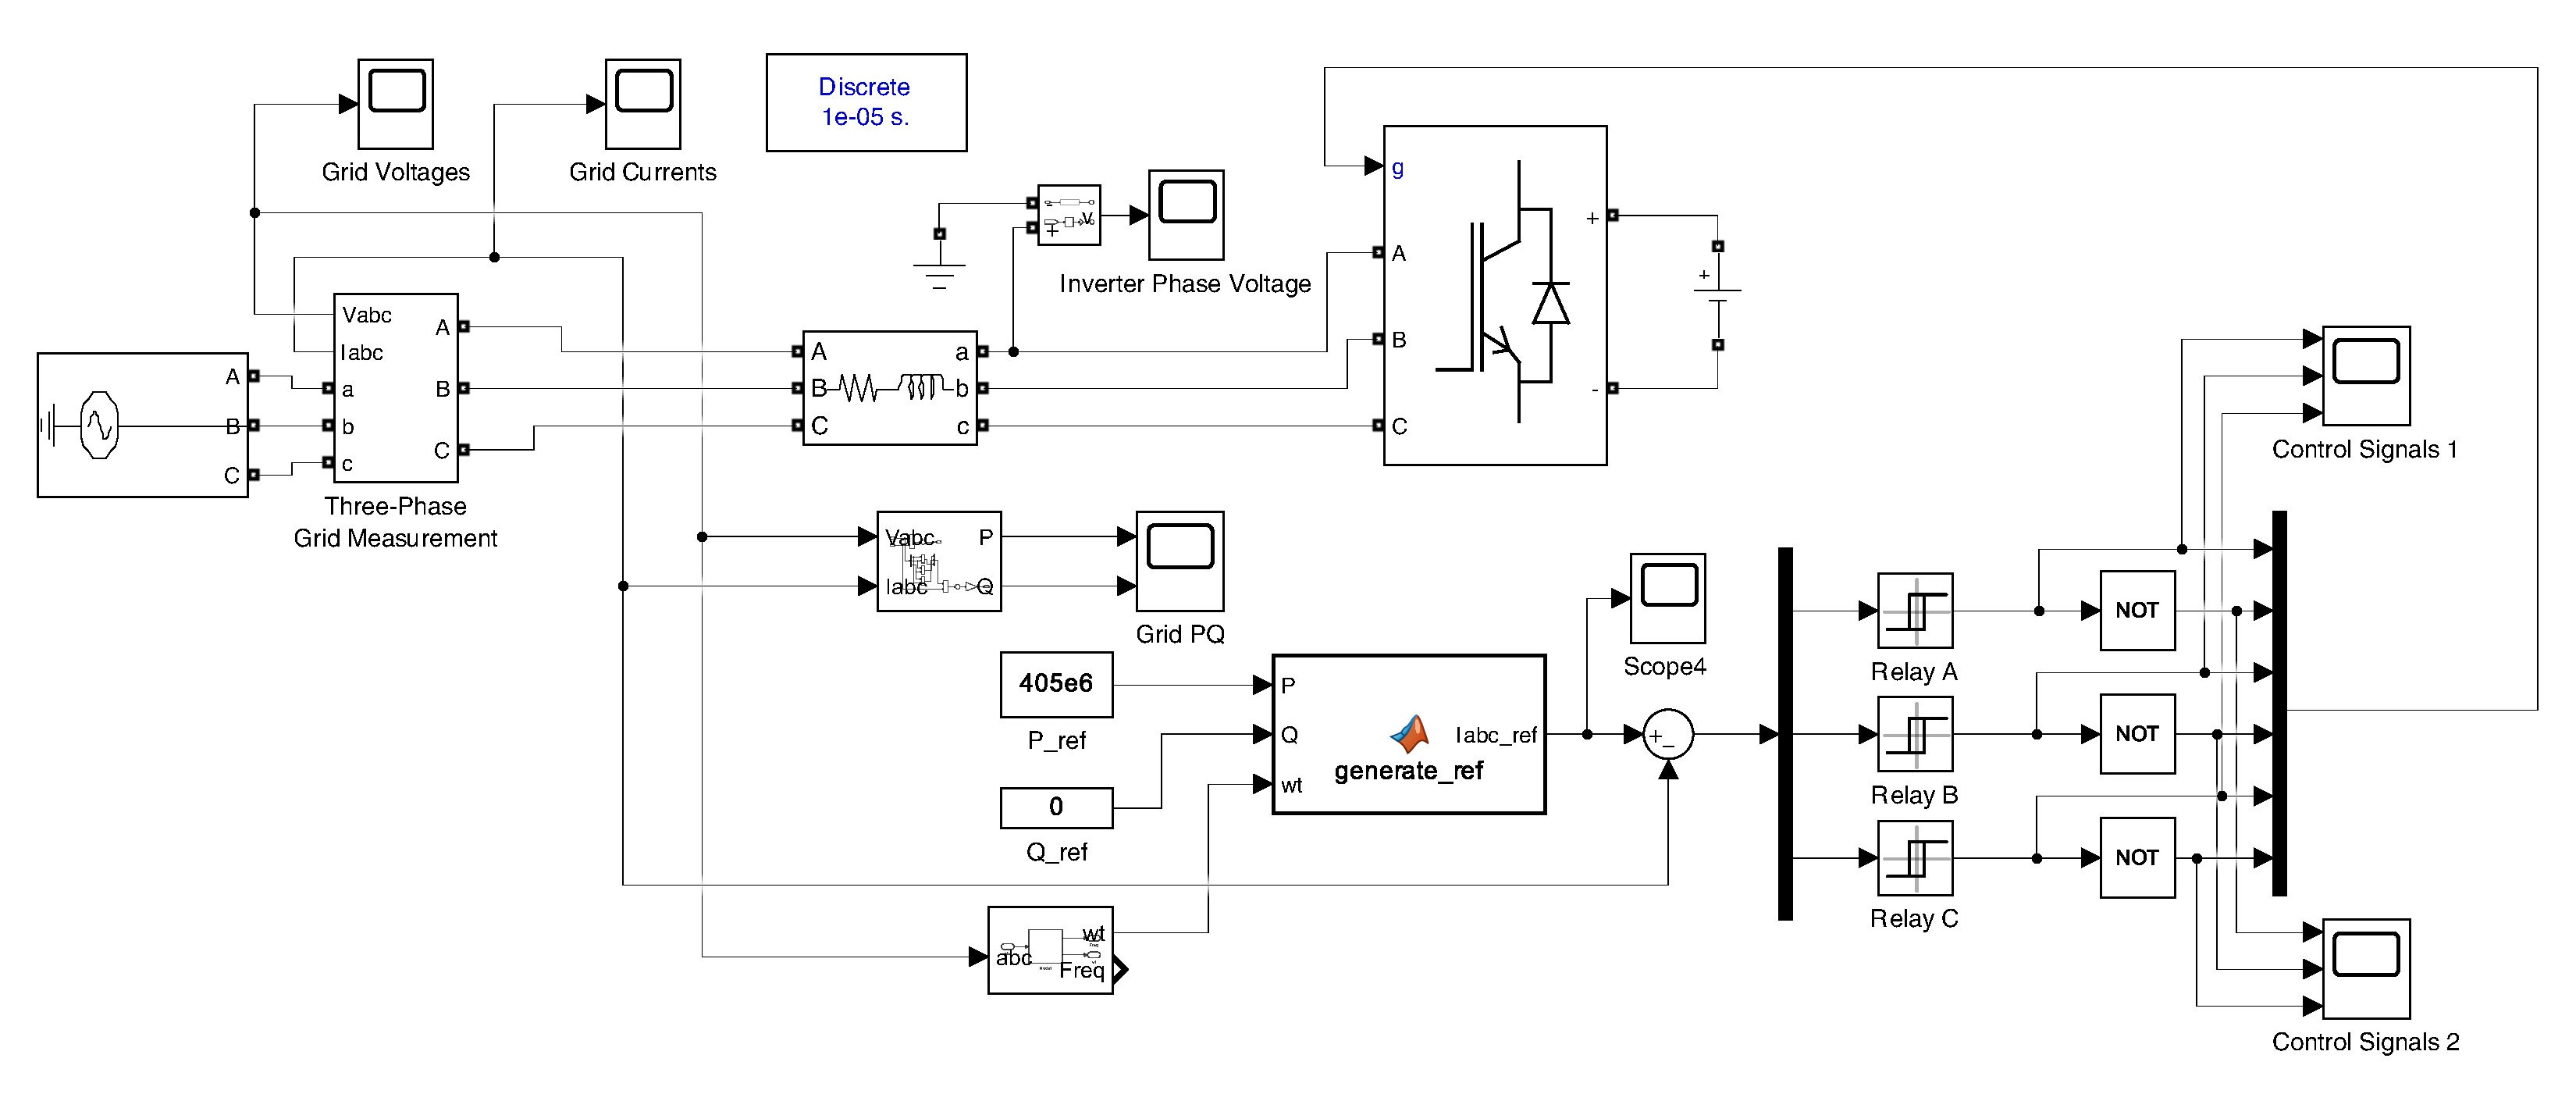
\includegraphics[width=\textwidth]{Full_Sys.jpg}
    \caption{Complete Simulink Model of the Two-Level VSC System.}
\end{figure}

\newpage
% ---------------- SECTION 2: CONTROL STRATEGY ---------------- %
\section{Control Strategy}
The control strategy relies on a Hysteresis Current Controller operating directly in the $abc$ reference frame. This non-linear feedback control method is renowned for its outstanding dynamic response, unconditional stability, and simplicity in implementation, as it avoids complex inner current loop PI tuning and coordinate transformations ($dq0$).

\subsection{Reference Current Generation}
The reference currents ($I_{abc}^*$) are generated analytically based on the instantaneous required active and reactive power values. The theoretical magnitude of the reference phase current is calculated based on the apparent power equation:
\vspace{0.25cm}
\begin{equation}
    S = \sqrt{P^2 + Q^2}, \quad S = \frac{3}{2} V_m I_m \implies I_m = \frac{2}{3} \frac{S}{V_m}
\end{equation}
\vspace{0.25cm}
Where $V_m$ is the peak phase voltage ($90\text{ kV}$). The power factor angle, defining the phase shift between the grid voltage and the injected current, is determined by $\phi = \tan^{-1}(Q/P)$. The following MATLAB function was utilized in the simulation to continuously generate the instantaneous synchronized reference signals:

\begin{lstlisting}
function Iabc_ref = generate_ref(P, Q, wt)
    Vm = 90000; % Peak phase voltage
    
    % Calculate peak current
    S = sqrt(P^2 + Q^2);
    Im = (2/3) * (S / Vm);
    
    % Calculate power factor angle
    phi = atan2(Q, P);
    
    % Generate 3-phase reference currents
    Ia = Im * sin(wt - phi);
    Ib = Im * sin(wt - 2*pi/3 - phi);
    Ic = Im * sin(wt + 2*pi/3 - phi);
    
    Iabc_ref = [Ia; Ib; Ic];
end
\end{lstlisting}
\newpage
\subsection{Hysteresis Current Control and Gate Signals}
The generated reference currents are continuously compared with the actual measured grid currents. The resulting error signal, $e(t) = i^*(t) - i(t)$, is fed into Relay blocks with a predefined tolerance band ($\pm \Delta i$). 

When the actual current hits the upper limit of the hysteresis band, the upper IGBT of the corresponding leg is turned off, and the lower IGBT is turned on, forcing the current to decrease. Conversely, when it hits the lower limit, the switching state is reversed. This logic generates the switching pulses for the upper IGBTs. Logical NOT operators generate the complementary pulses for the lower IGBTs to avoid short-circuiting the DC link. While this method results in a variable switching frequency, it tightly bounds the current error, yielding excellent tracking capability.

\begin{figure}[H]
    \centering
    \begin{subfigure}{0.8\textwidth}
        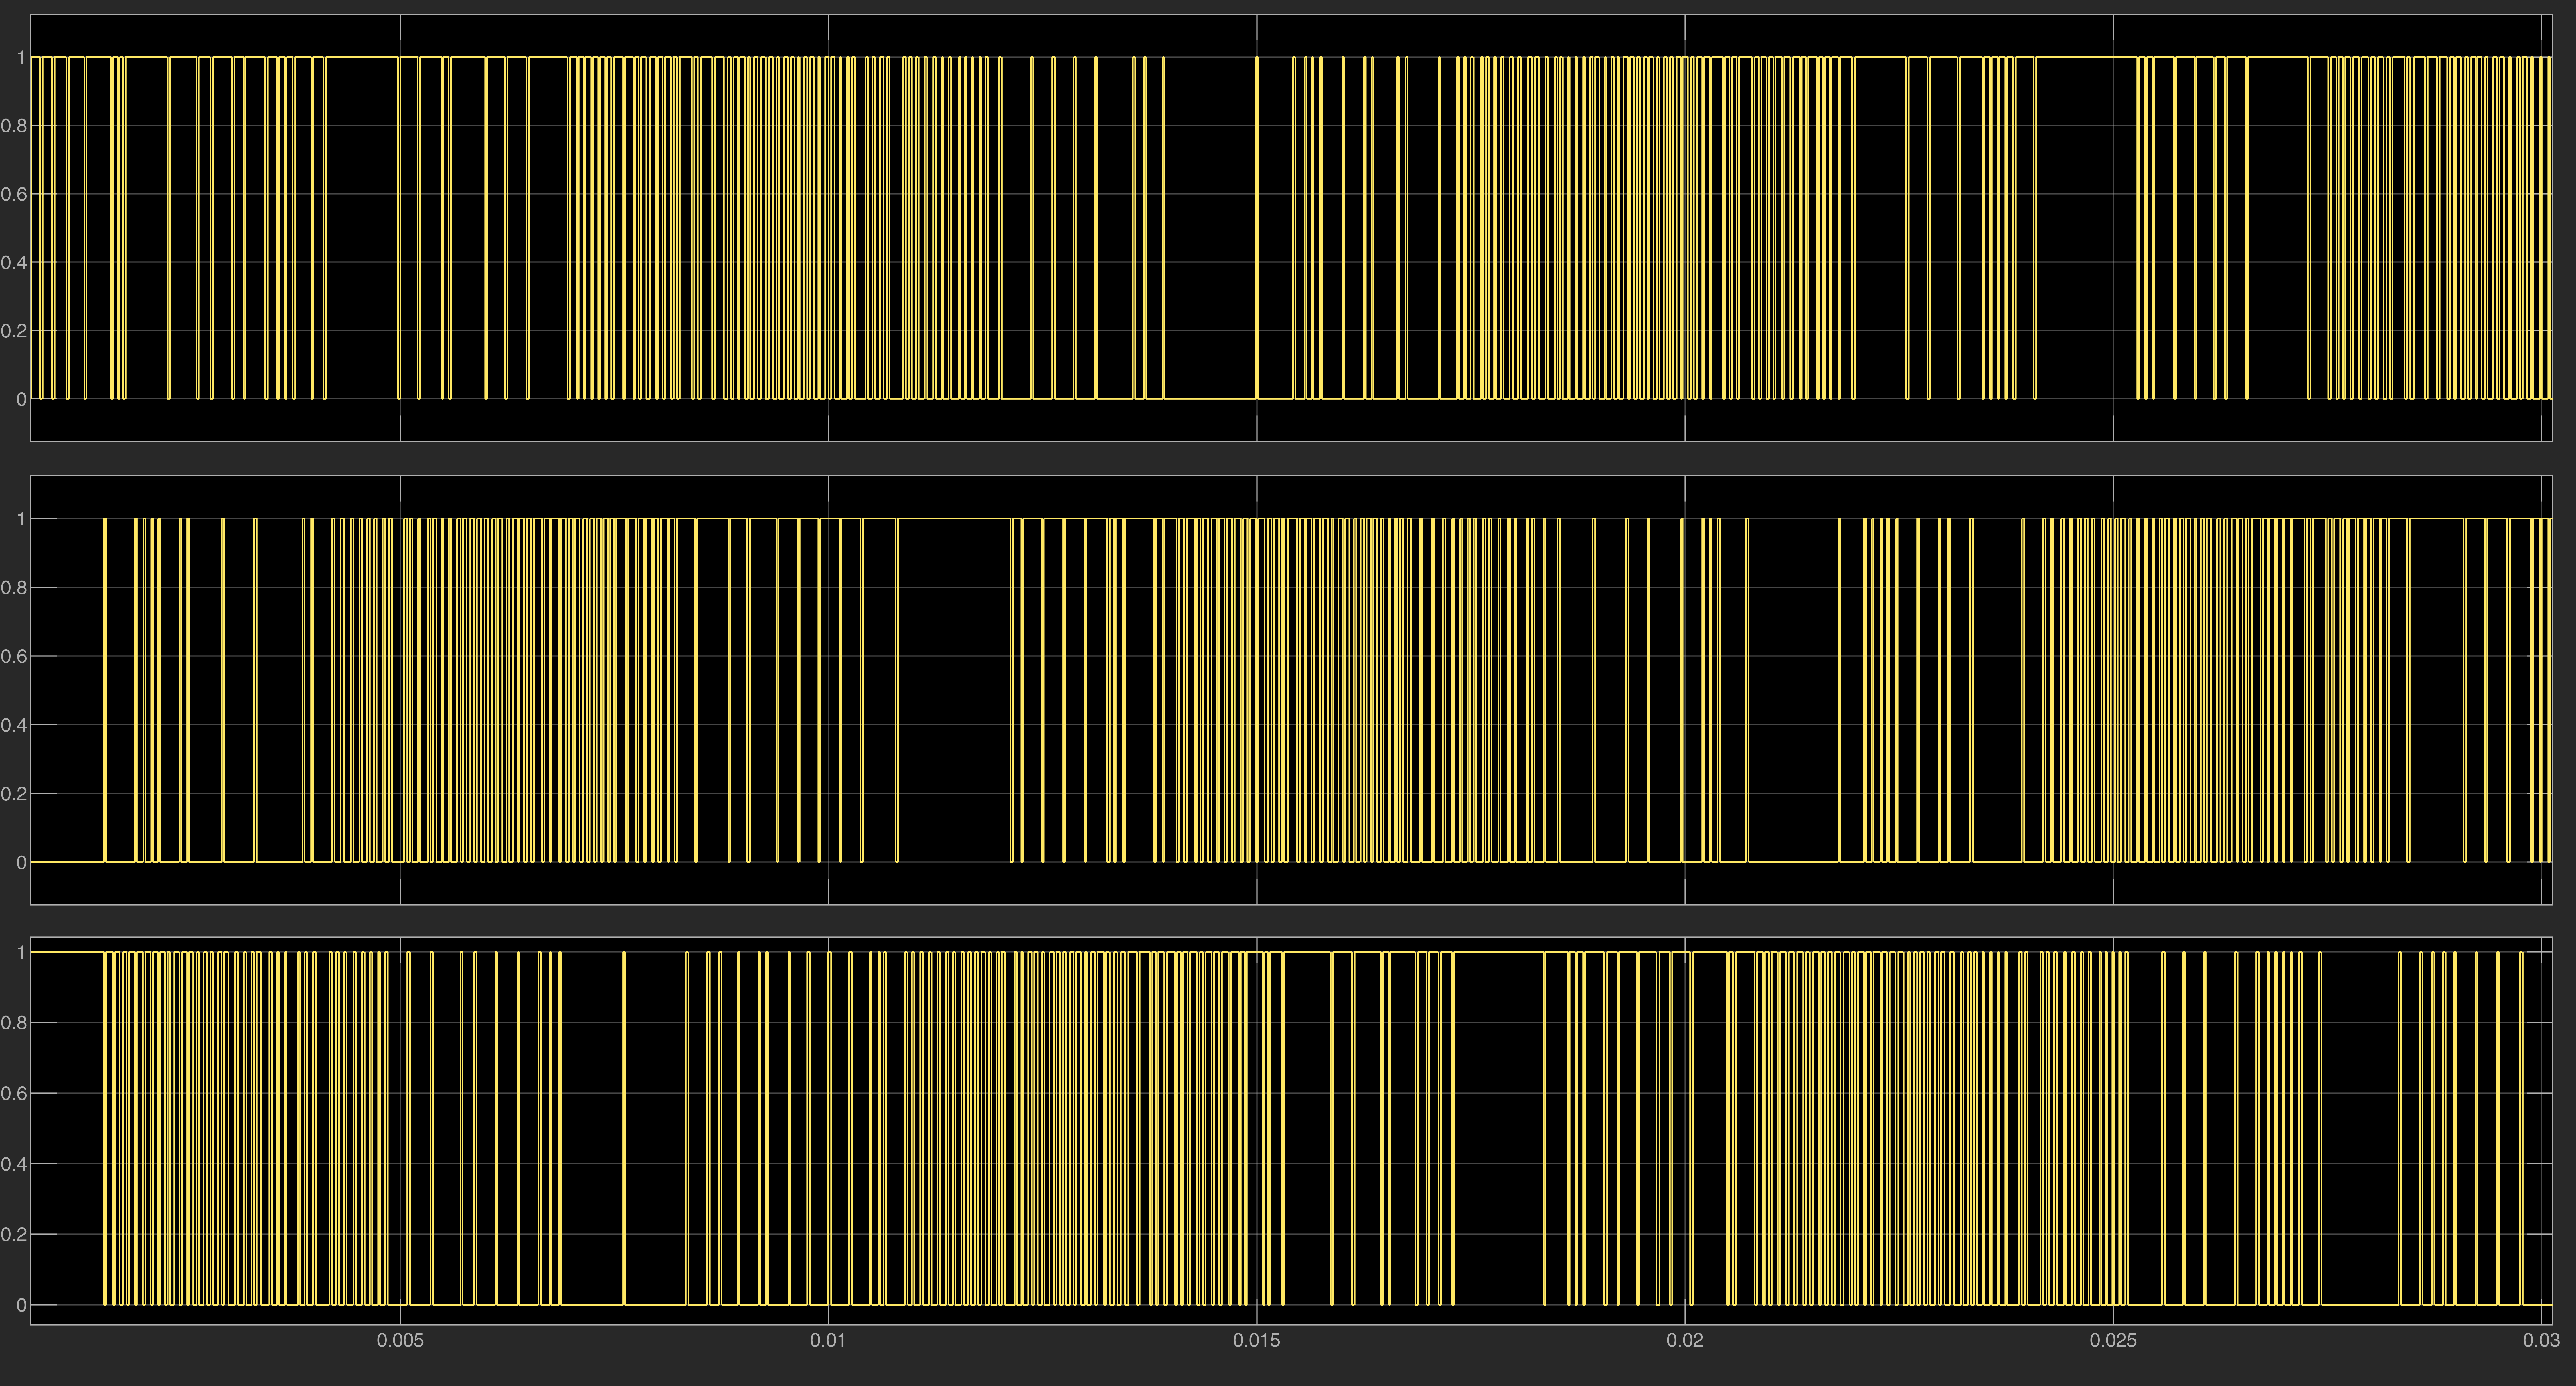
\includegraphics[width=\textwidth]{Controll + signals.png}
        \caption{Upper IGBTs Switching Signals}
    \end{subfigure}
    \vfill
    \begin{subfigure}{0.8\textwidth}
        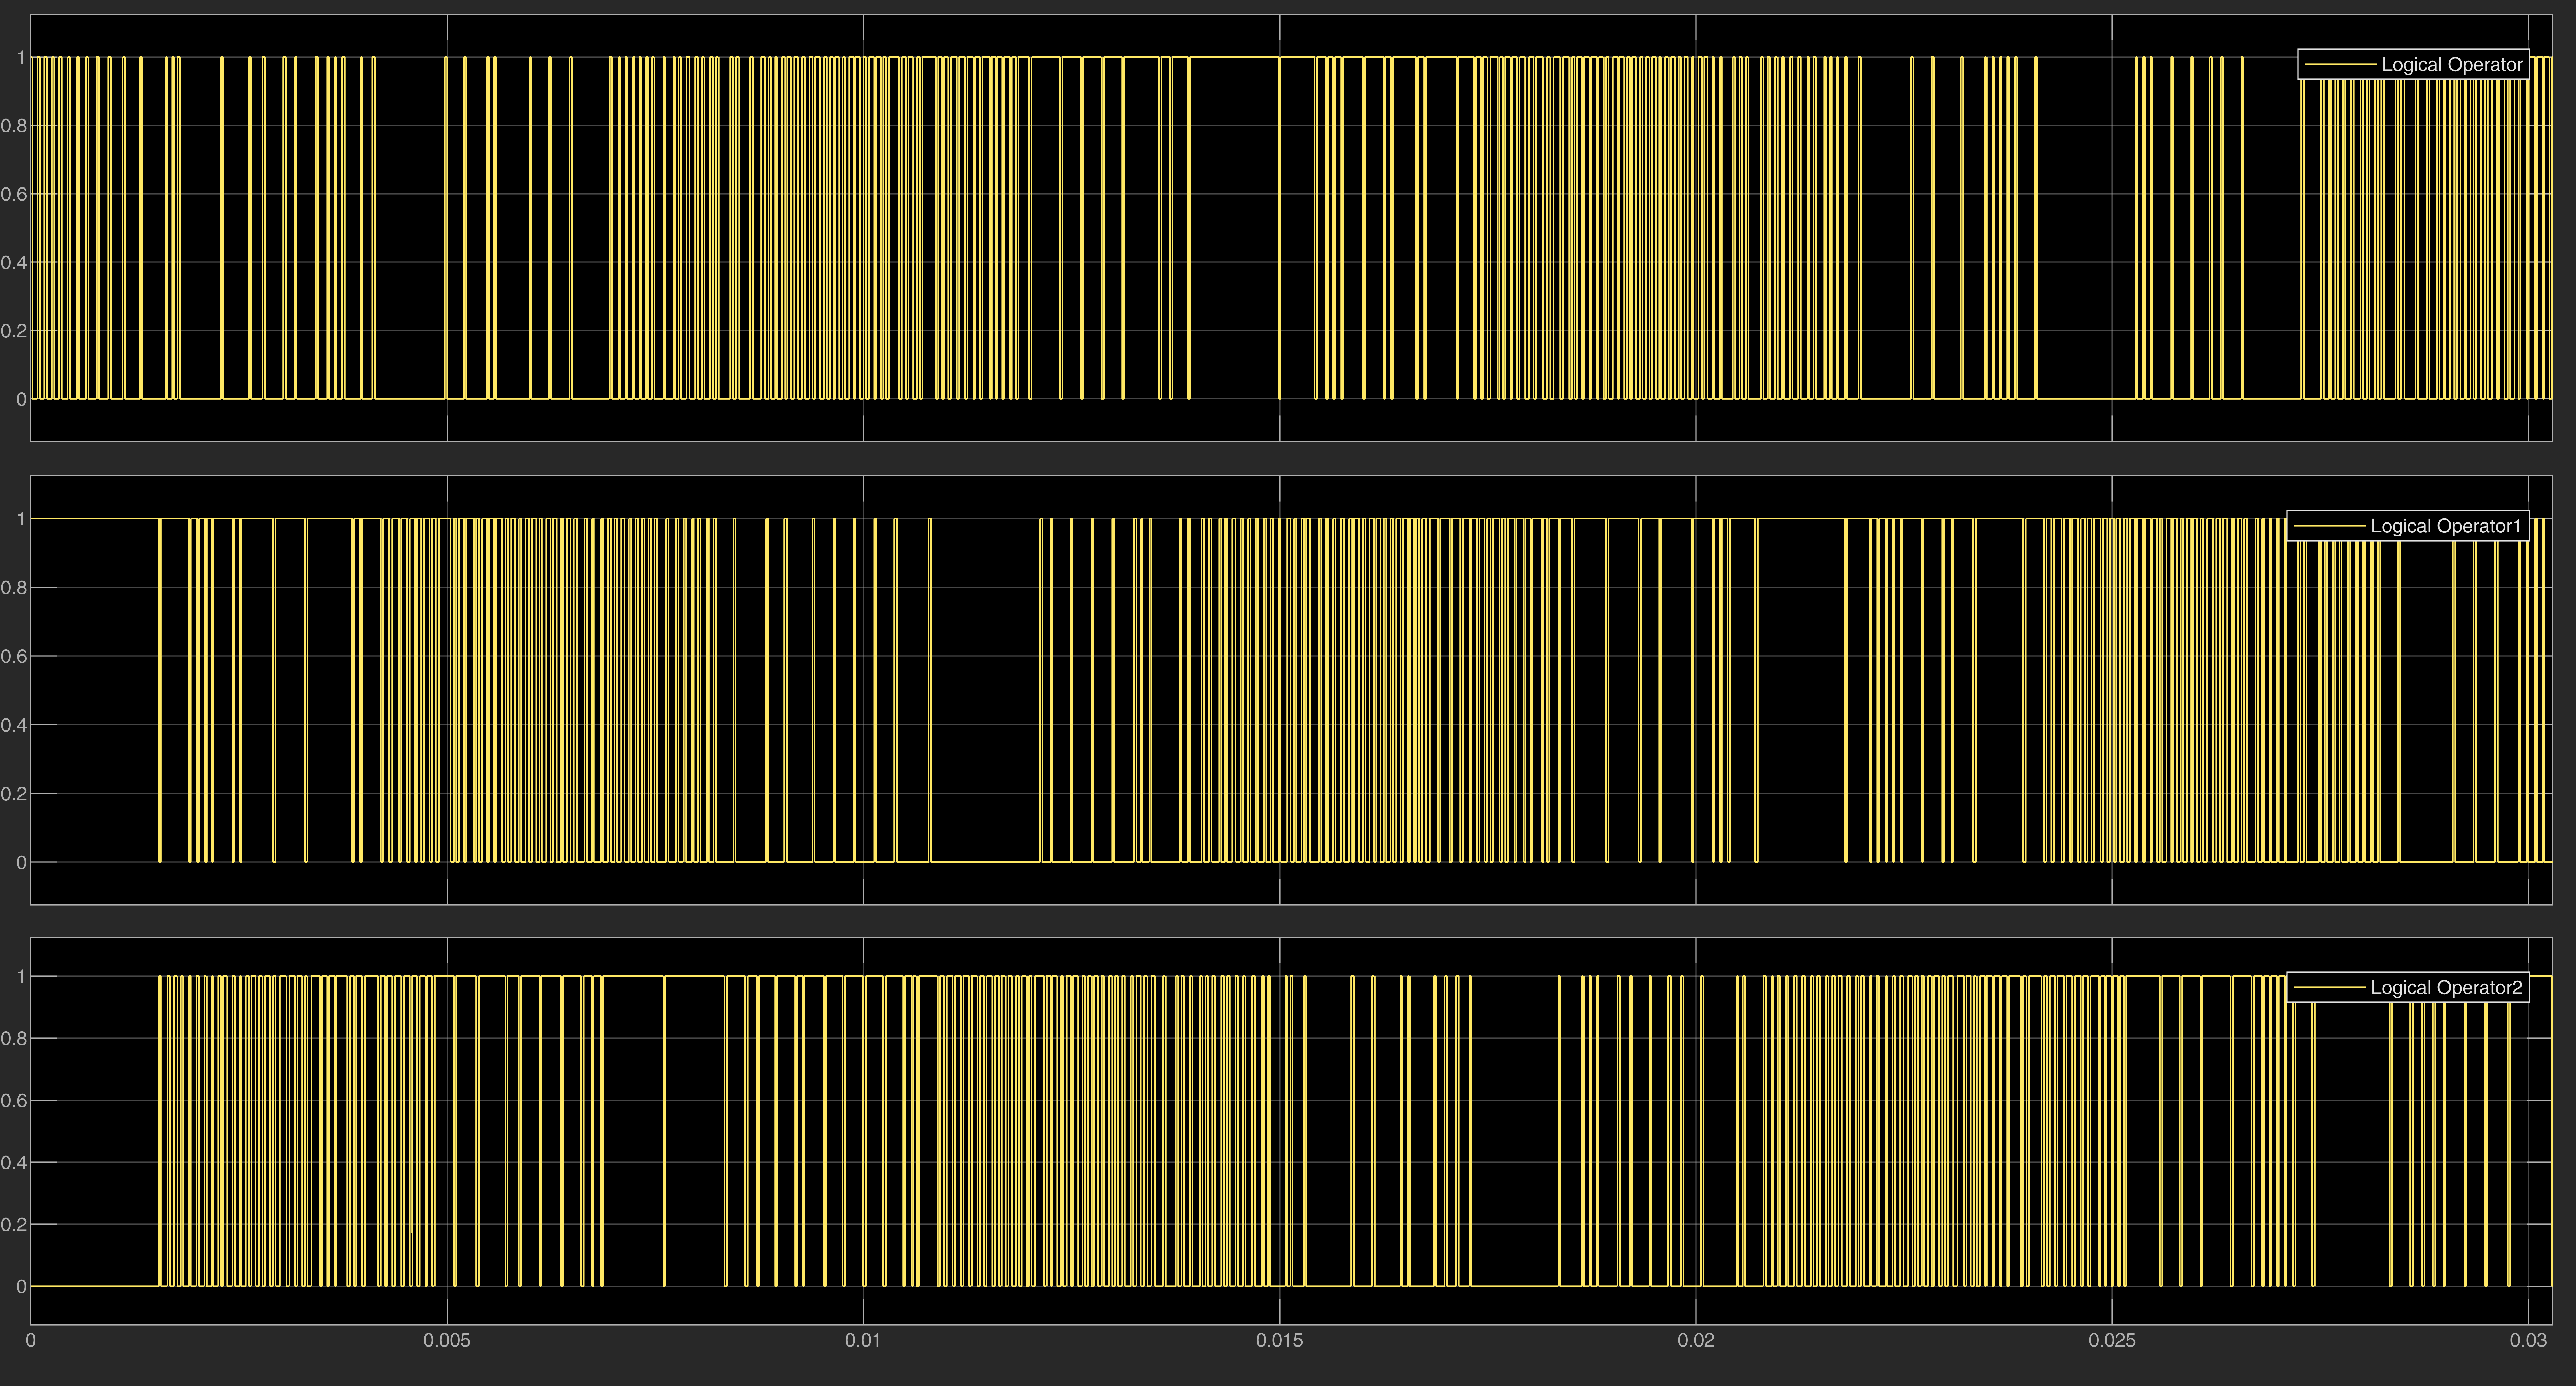
\includegraphics[width=\textwidth]{Controll - signals.png}
        \caption{Lower IGBTs Complementary Switching Signals}
    \end{subfigure}
    \caption{Complementary PWM Gate Signals generated by the Hysteresis Controller.}
\end{figure}

\newpage
% ---------------- SECTION 3: SIMULATION CASES ---------------- %
\section{Simulation Results and Analysis}
To thoroughly evaluate the performance of the implemented VSC and its hysteresis controller, the system was subjected to five distinct operational cases, covering steady-state operations at various power factors and a severe dynamic transient.

% --- Case 1 ---
\subsection{Case 1: Injection of +405 MW and 0 MVAR}
In this baseline scenario, the VSC operates at unity power factor, injecting purely active power into the grid. The reactive power is strictly maintained at zero, which is the ideal condition to minimize transmission line losses and maximize the active power transfer capacity of the grid infrastructure. 

As observed in the waveforms, the grid current is in phase with the grid voltage, verifying the unity power factor operation. Based on the theoretical calculations, the peak phase current is expected to be $3000\text{ A}$ $\left( I_m = \frac{2}{3} \times \frac{405\text{ MVA}}{90\text{ kV}} \right)$, which matches the simulation output. The inverter phase voltage exhibits a clean two-level PWM characteristic, confirming proper switching action by the Hysteresis controller as it successfully bounds the actual current around the sinusoidal reference.

\begin{figure}[H]
    \centering
    \begin{subfigure}{0.48\textwidth}
        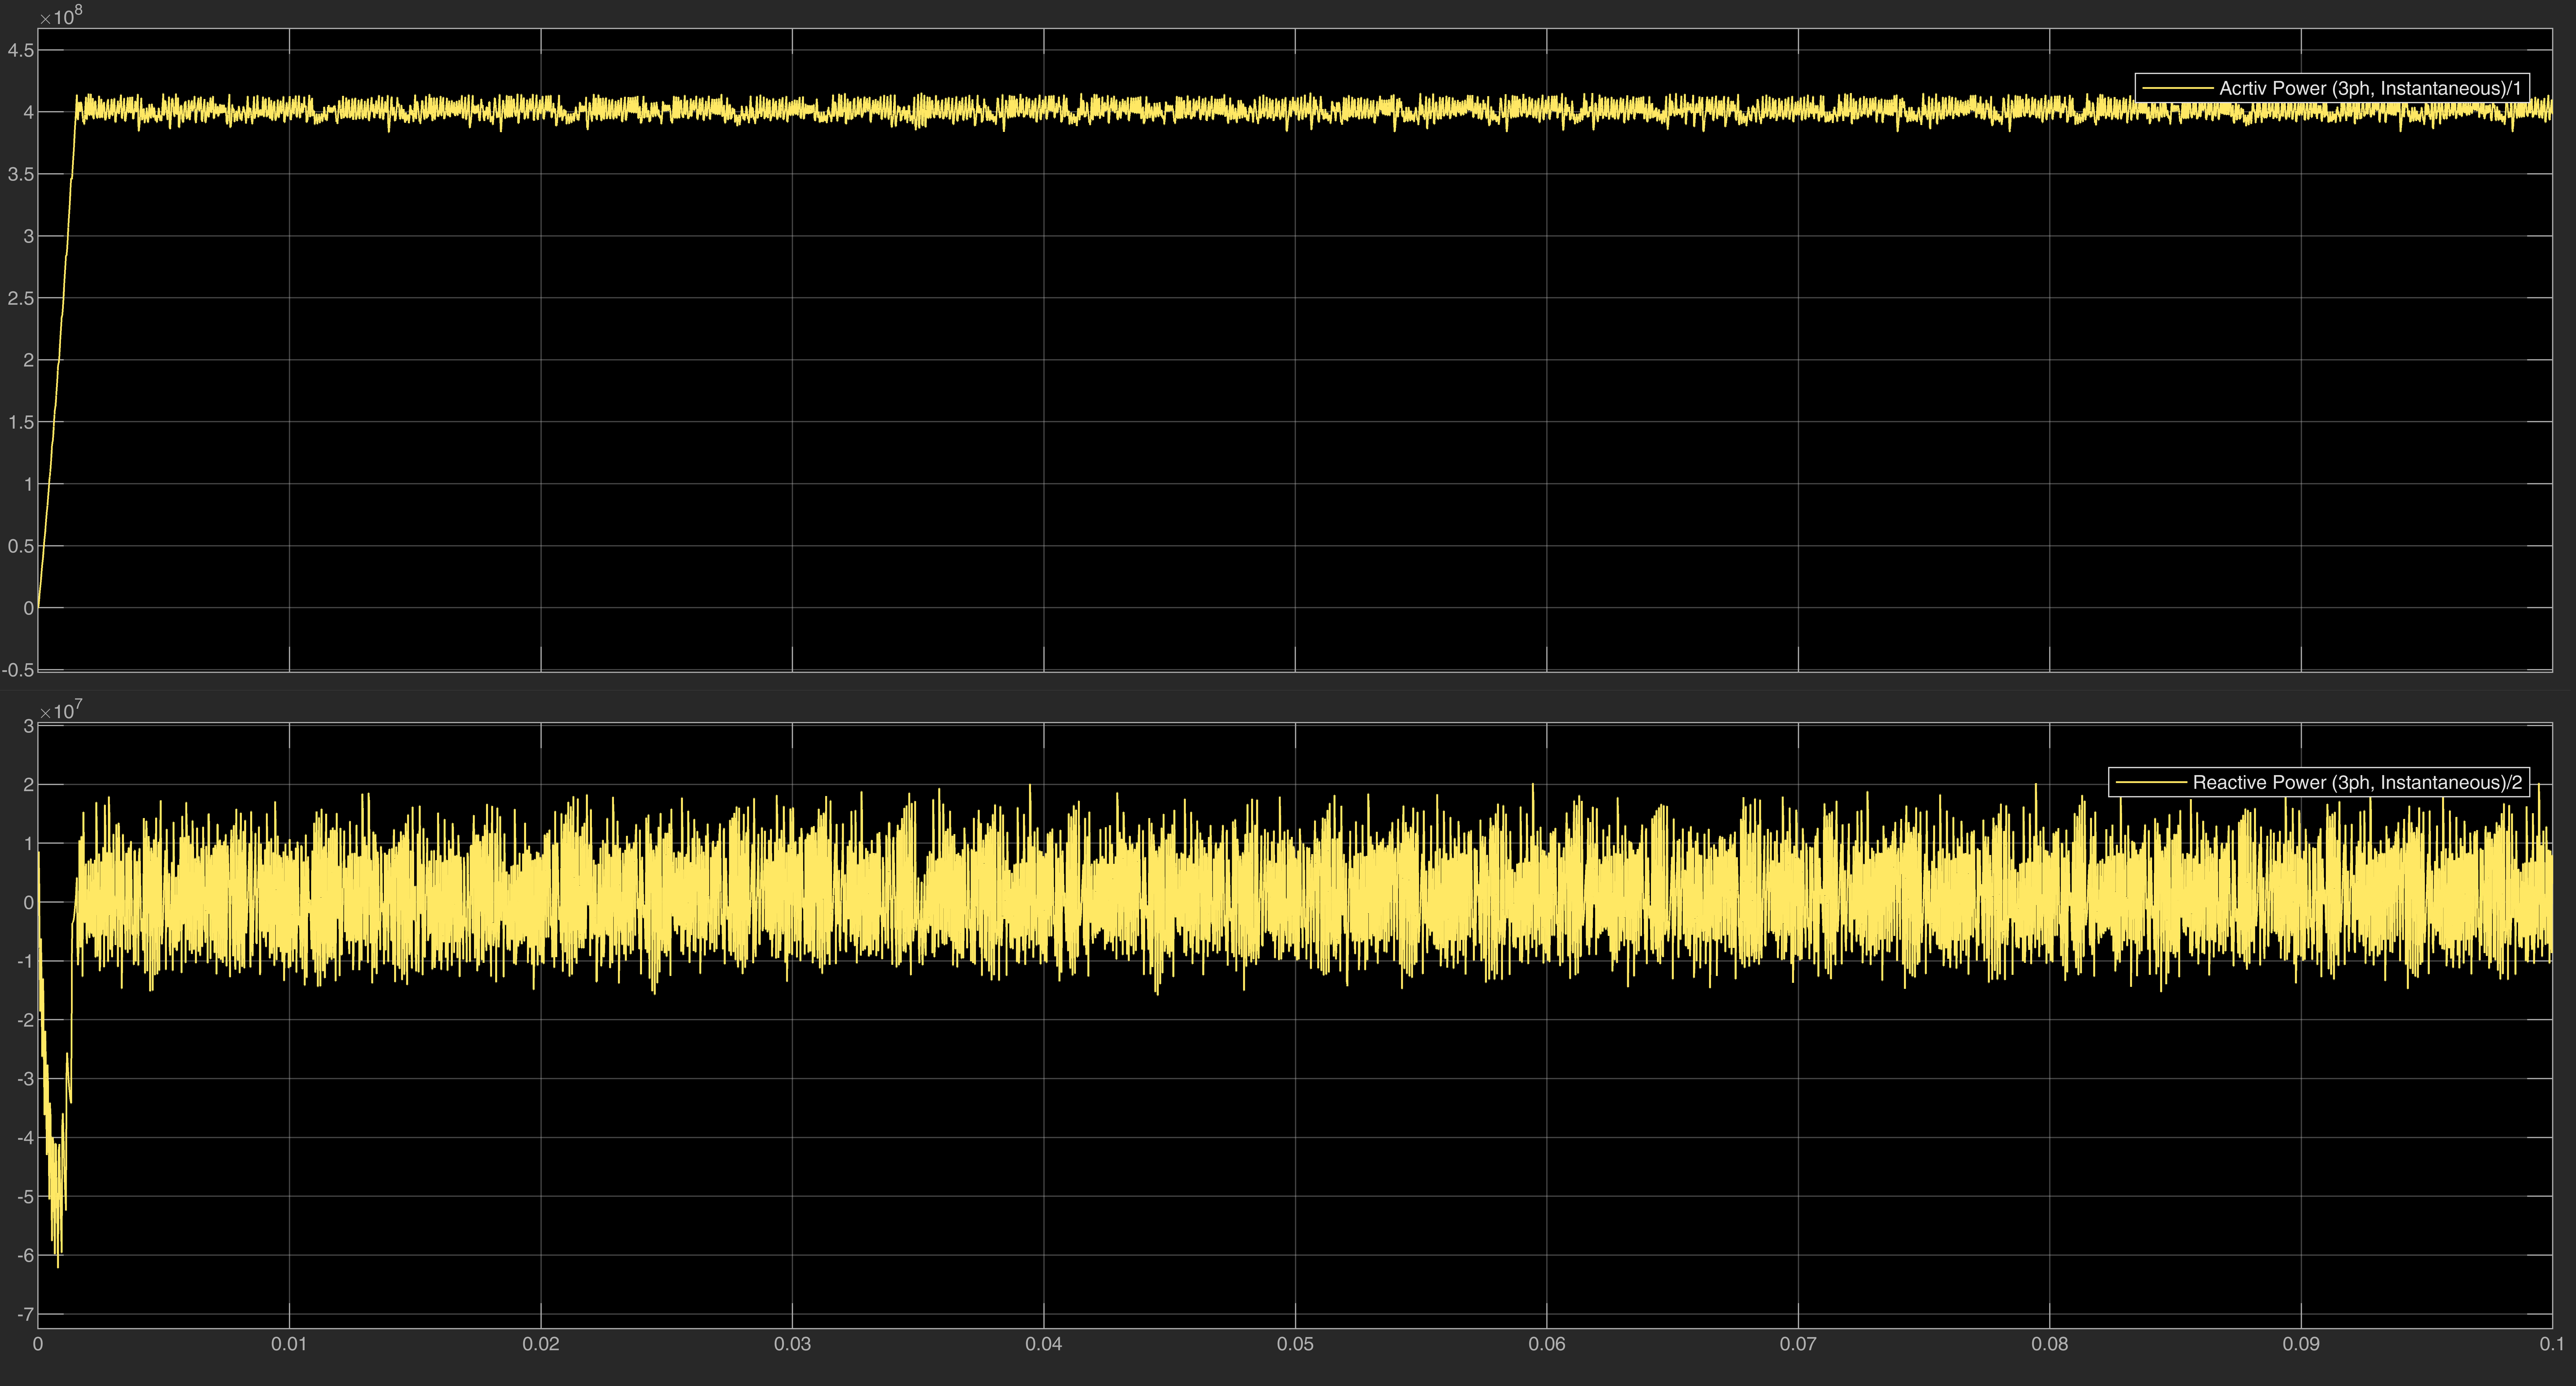
\includegraphics[width=\textwidth]{Grid active and reactive powers_1.png}
        \caption{Active and Reactive Power}
    \end{subfigure}
    \hfill
    \begin{subfigure}{0.48\textwidth}
        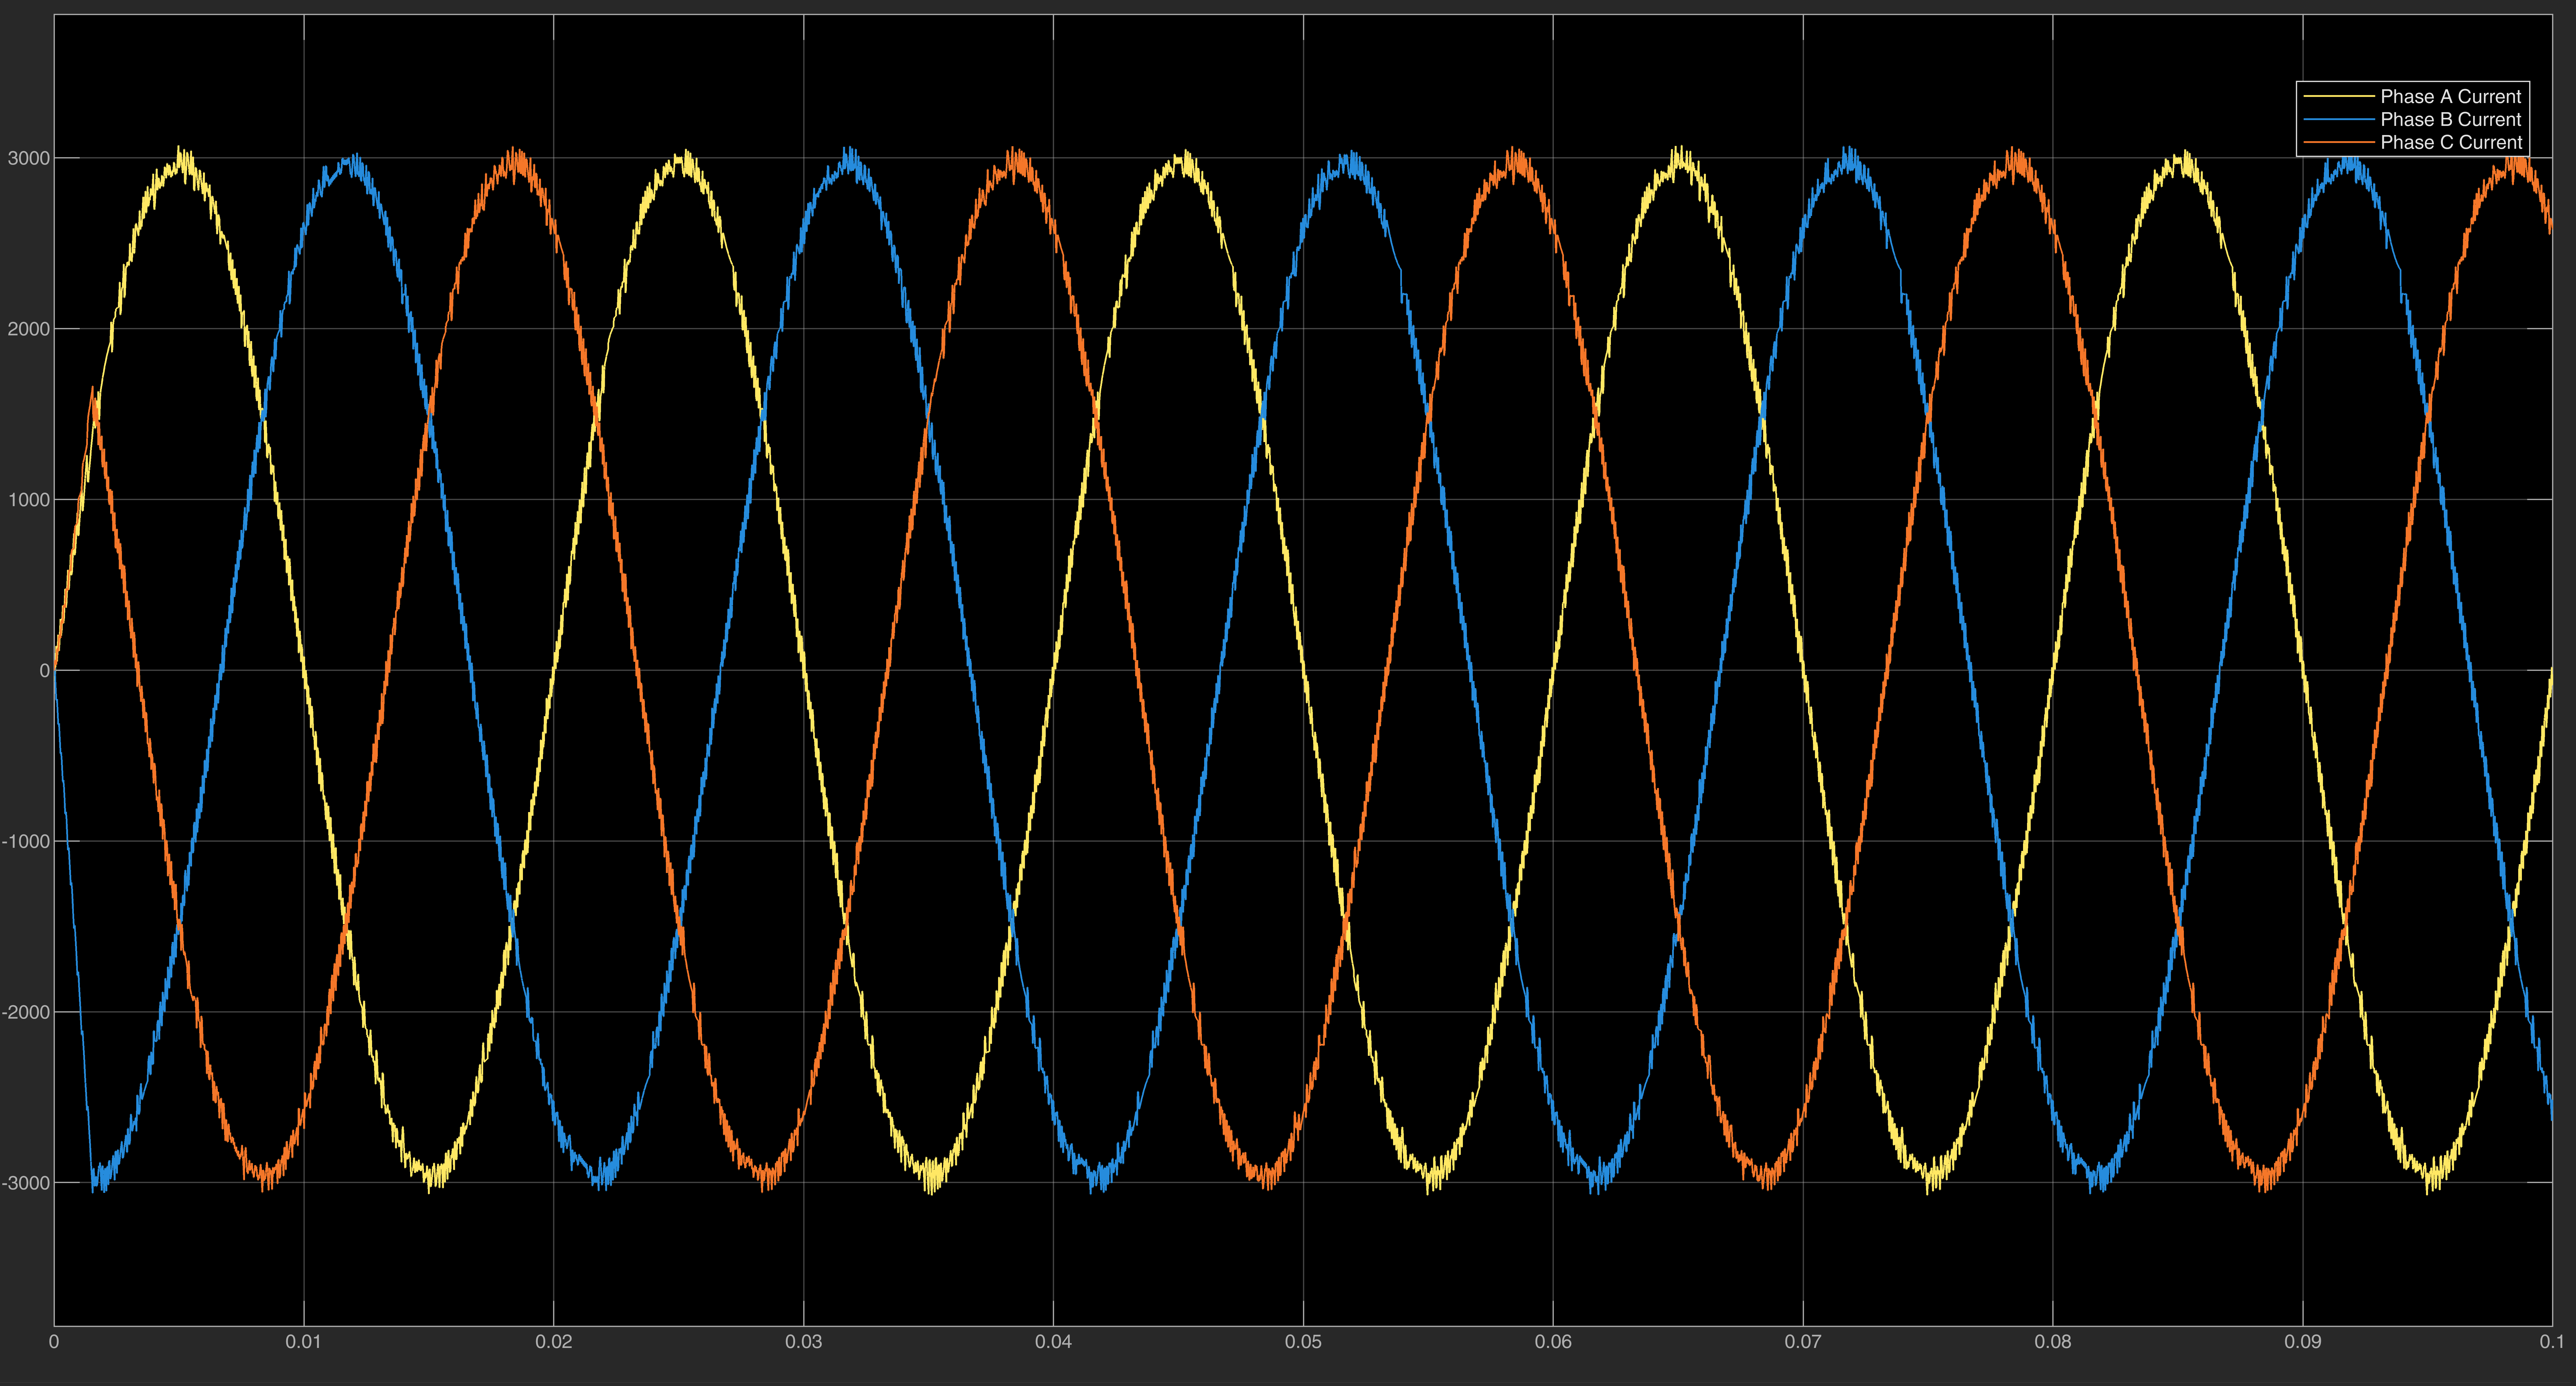
\includegraphics[width=\textwidth]{Grid Currents_1.png}
        \caption{Grid Currents}
    \end{subfigure}
    \vskip\baselineskip
    \begin{subfigure}{0.48\textwidth}
        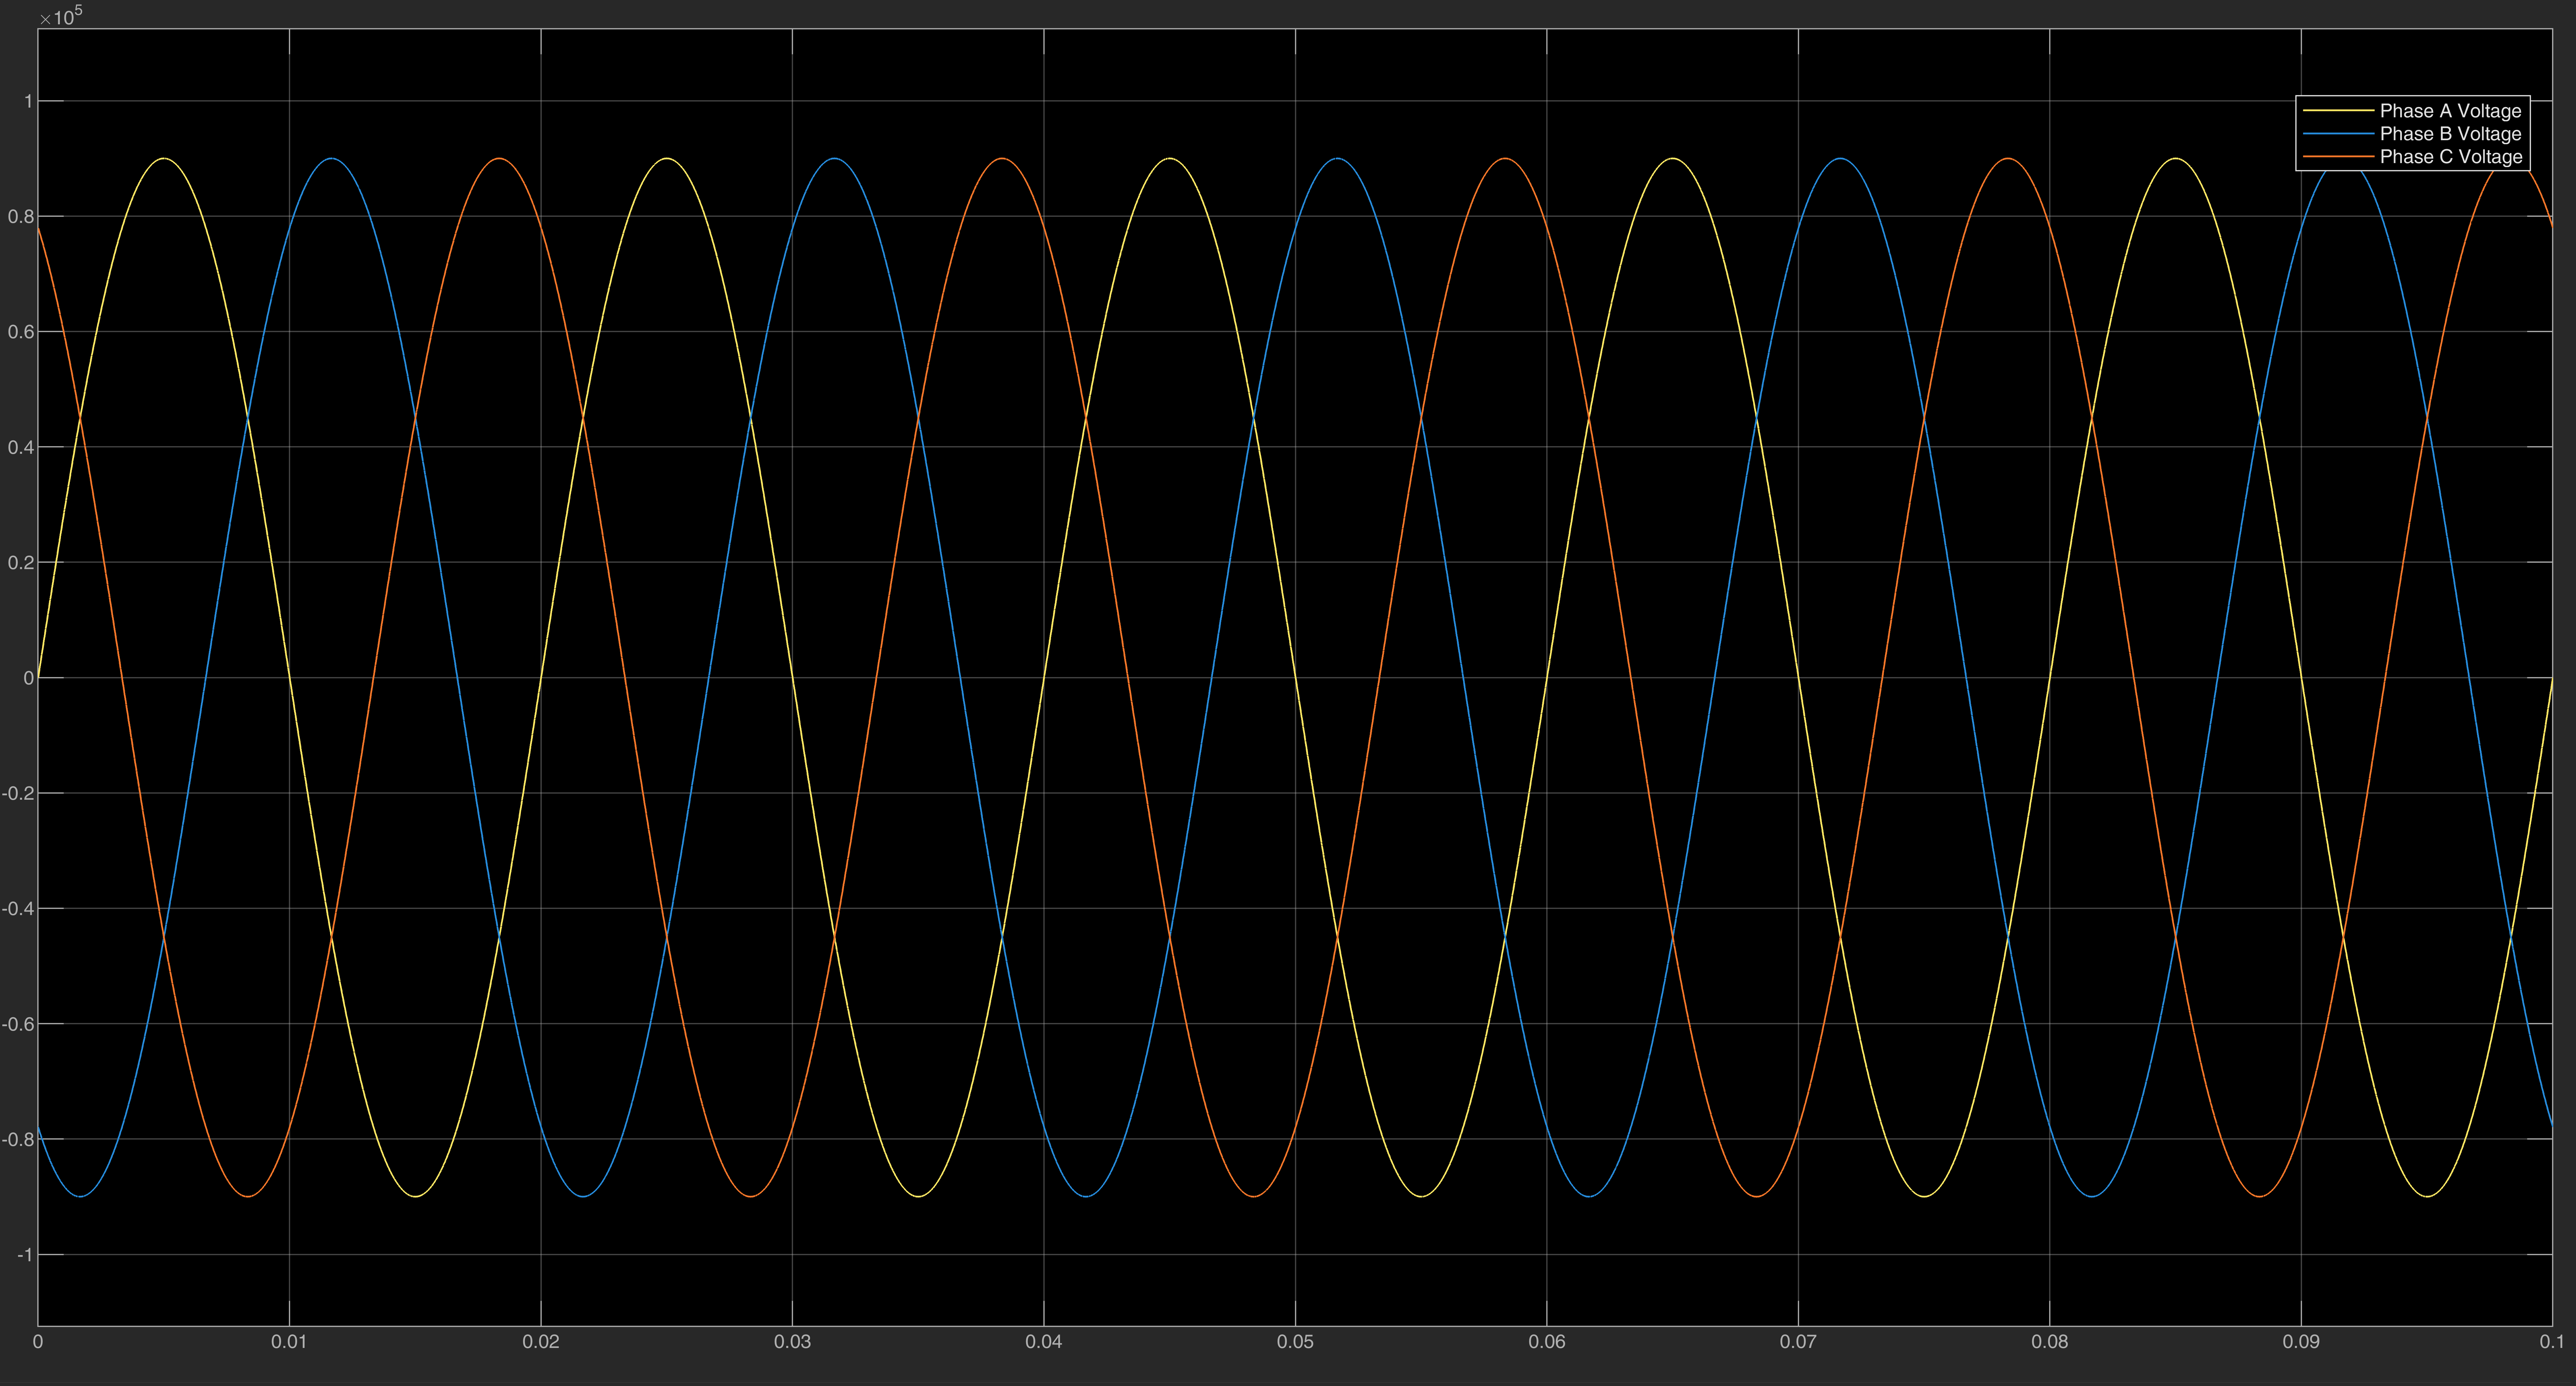
\includegraphics[width=\textwidth]{Grid Voltage_1.png}
        \caption{Grid Voltages}
    \end{subfigure}
    \hfill
    \begin{subfigure}{0.48\textwidth}
        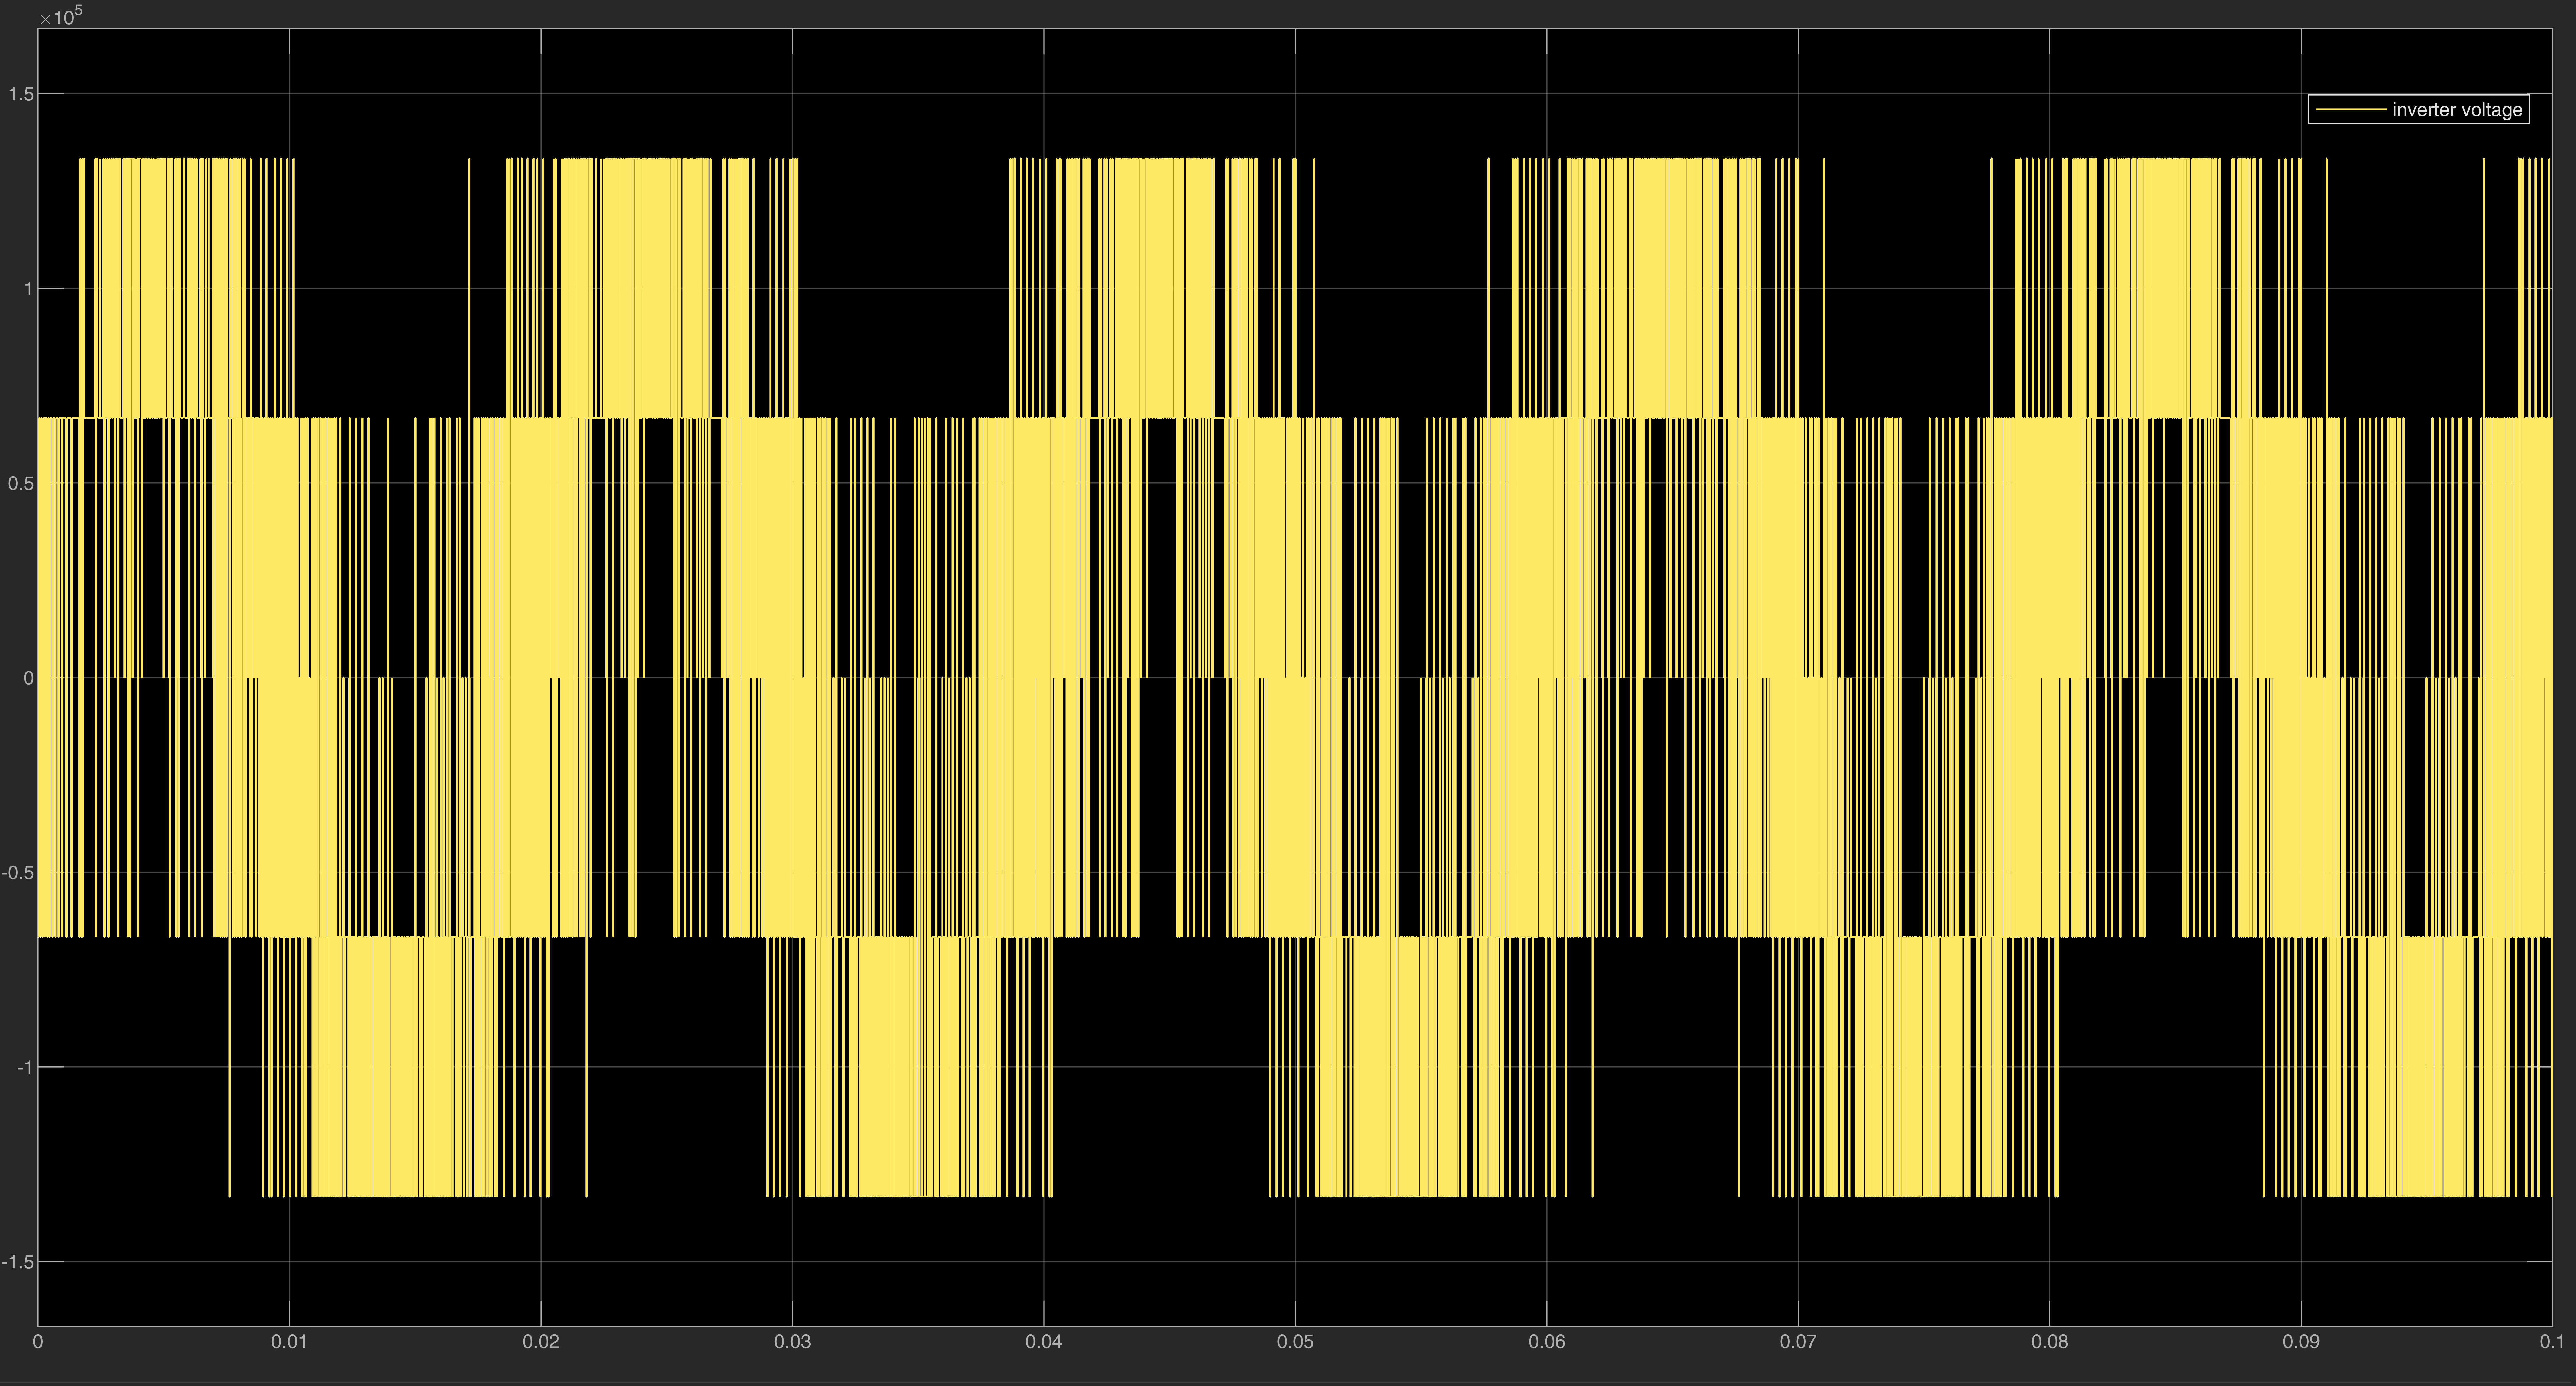
\includegraphics[width=\textwidth]{Inverter Phase Voltage_1.png}
        \caption{Inverter Phase Voltage}
    \end{subfigure}
    \caption{Simulation waveforms for Case 1 (Unity Power Factor).}
\end{figure}

\newpage

% --- Case 2 ---
\subsection{Case 2: Injection of +200 MW and +200 MVAR}
The system is commanded to deliver both active and reactive power symmetrically ($P = 200\text{ MW}$, $Q = 200\text{ MVAR}$). This case demonstrates the VSC's dual capability to act as an active power source while simultaneously functioning as a reactive power compensator to support local grid voltage profiles. 

Analytically, this equal distribution of real and reactive power results in a power factor angle of $45^\circ$. This theoretical angle is clearly visible as a precise phase displacement between the grid voltage and the injected current waveforms in the simulation. The apparent power required from the converter is $S = \sqrt{200^2 + 200^2} \approx 282.8\text{ MVA}$. This dictates a theoretical peak current of approximately $2095\text{ A}$, which the hysteresis controller tracks accurately without exceeding the designated switching band.

\begin{figure}[H]
    \centering
    \begin{subfigure}{0.48\textwidth}
        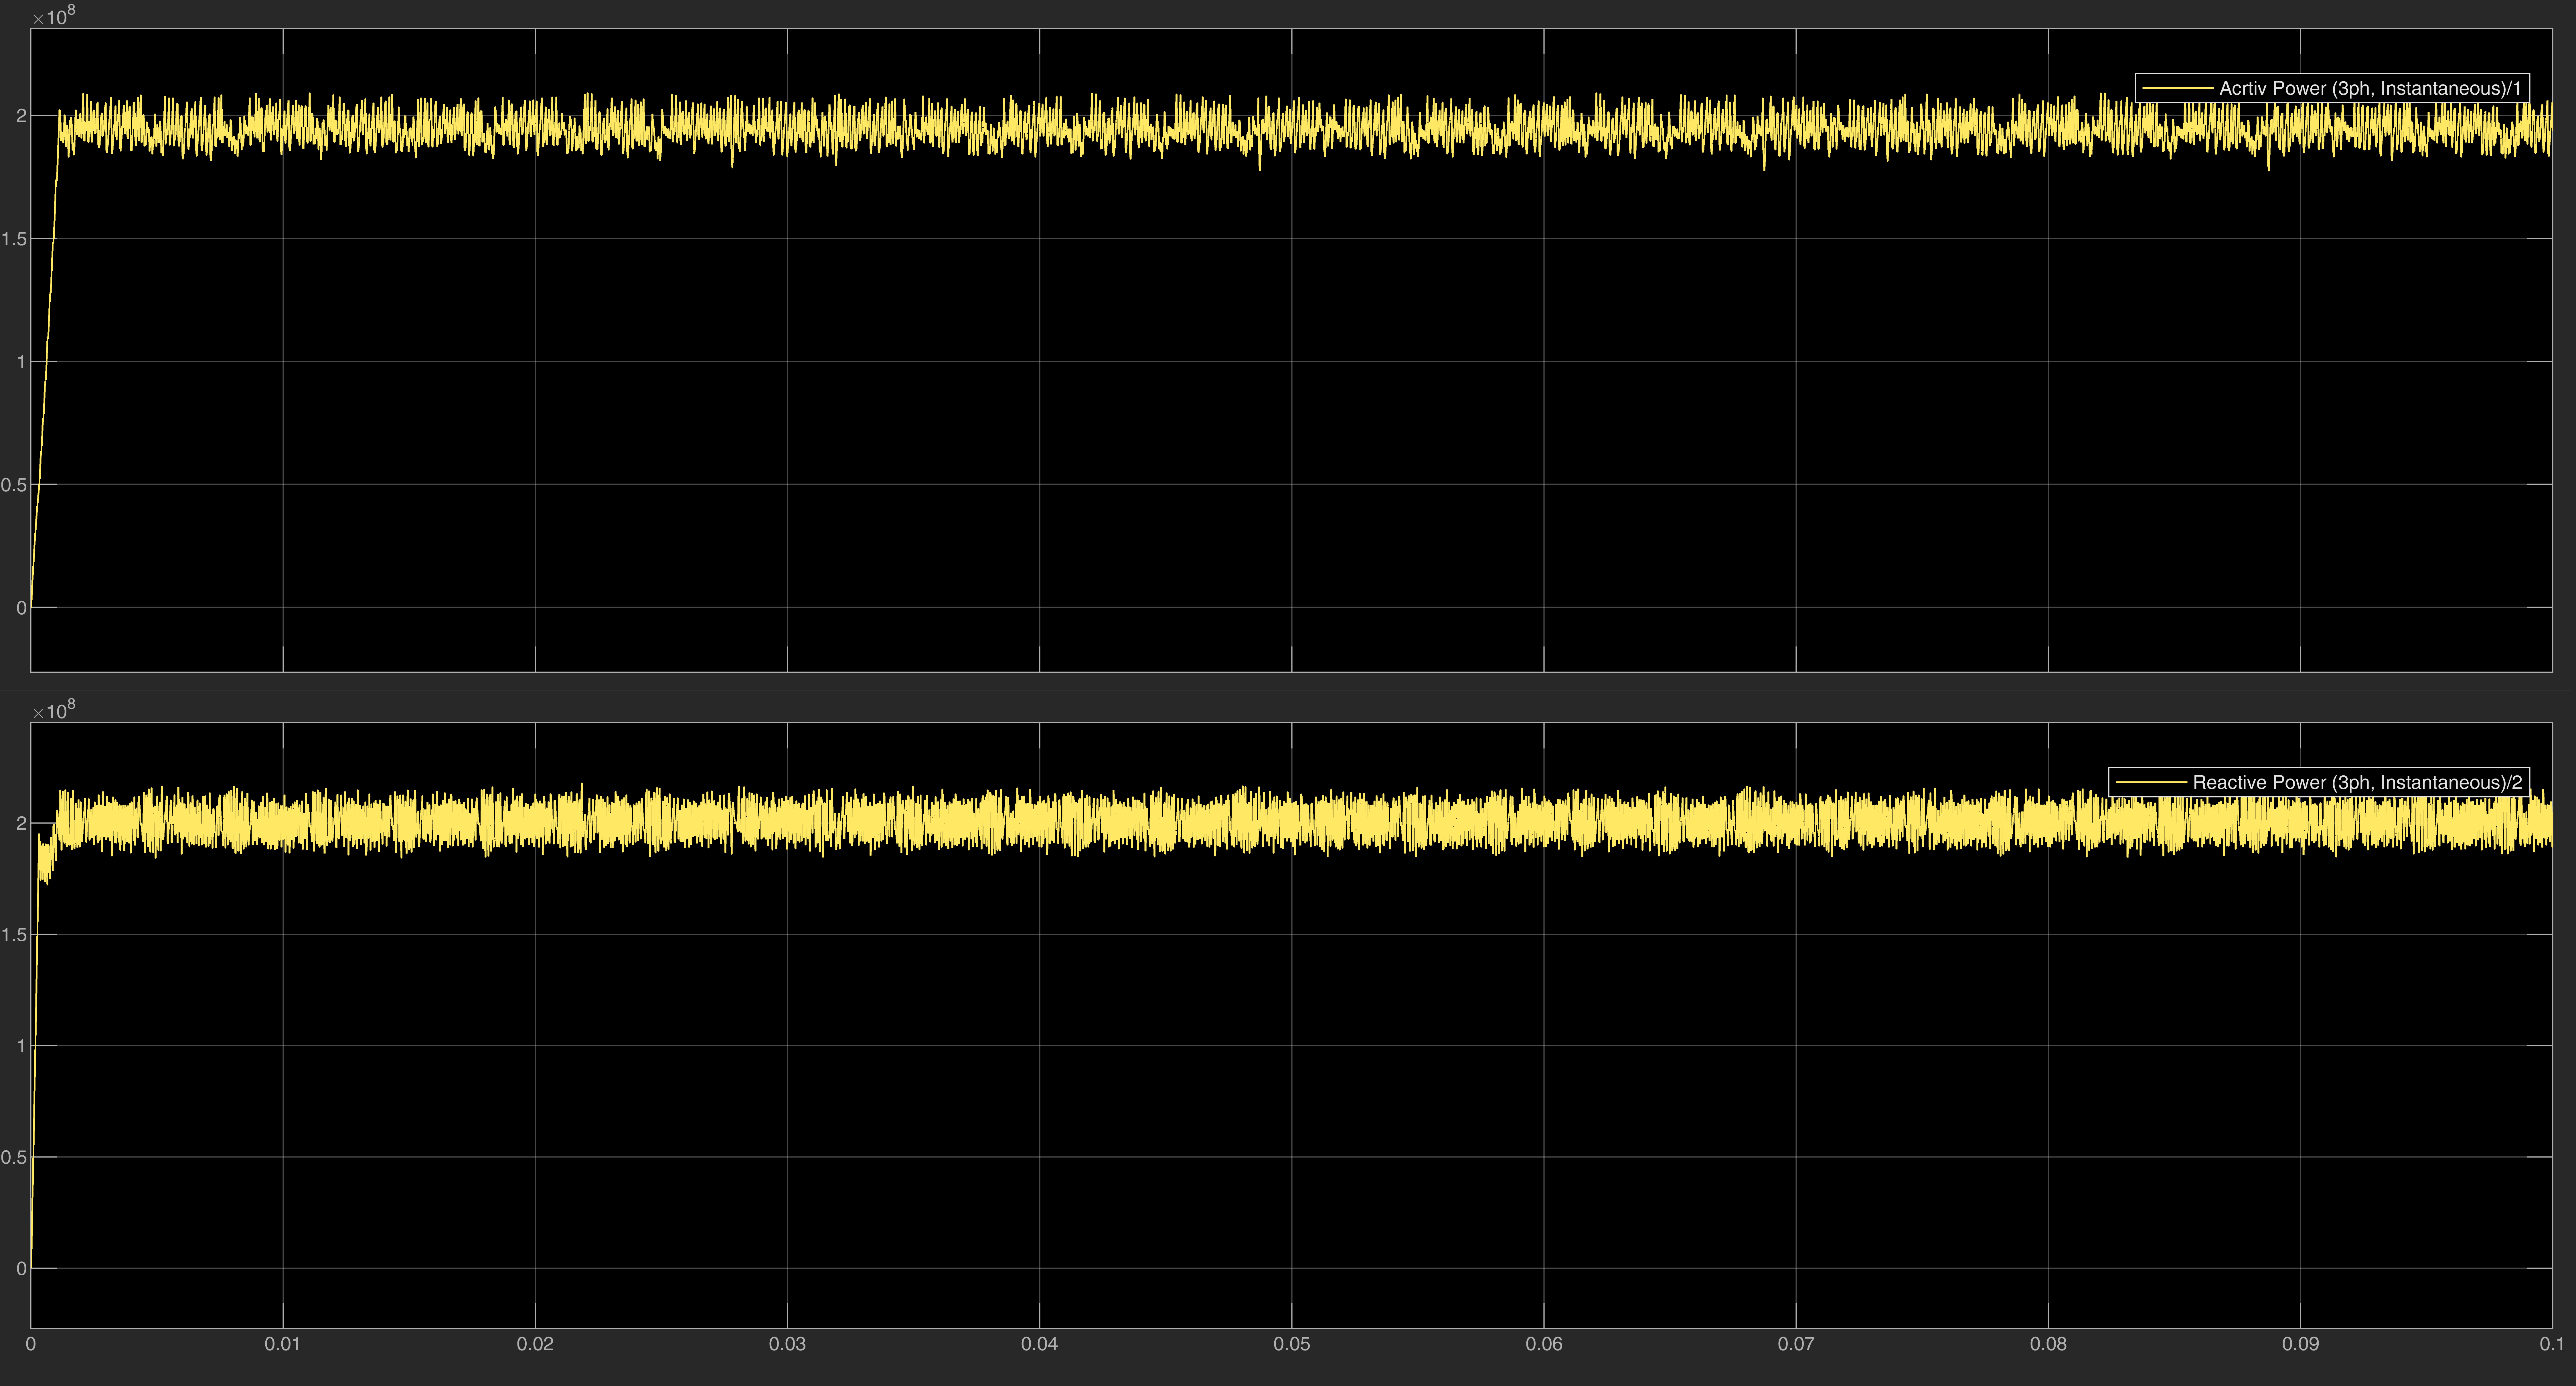
\includegraphics[width=\textwidth]{Grid active and reactive powers_2.png}
        \caption{Active and Reactive Power}
    \end{subfigure}
    \hfill
    \begin{subfigure}{0.48\textwidth}
        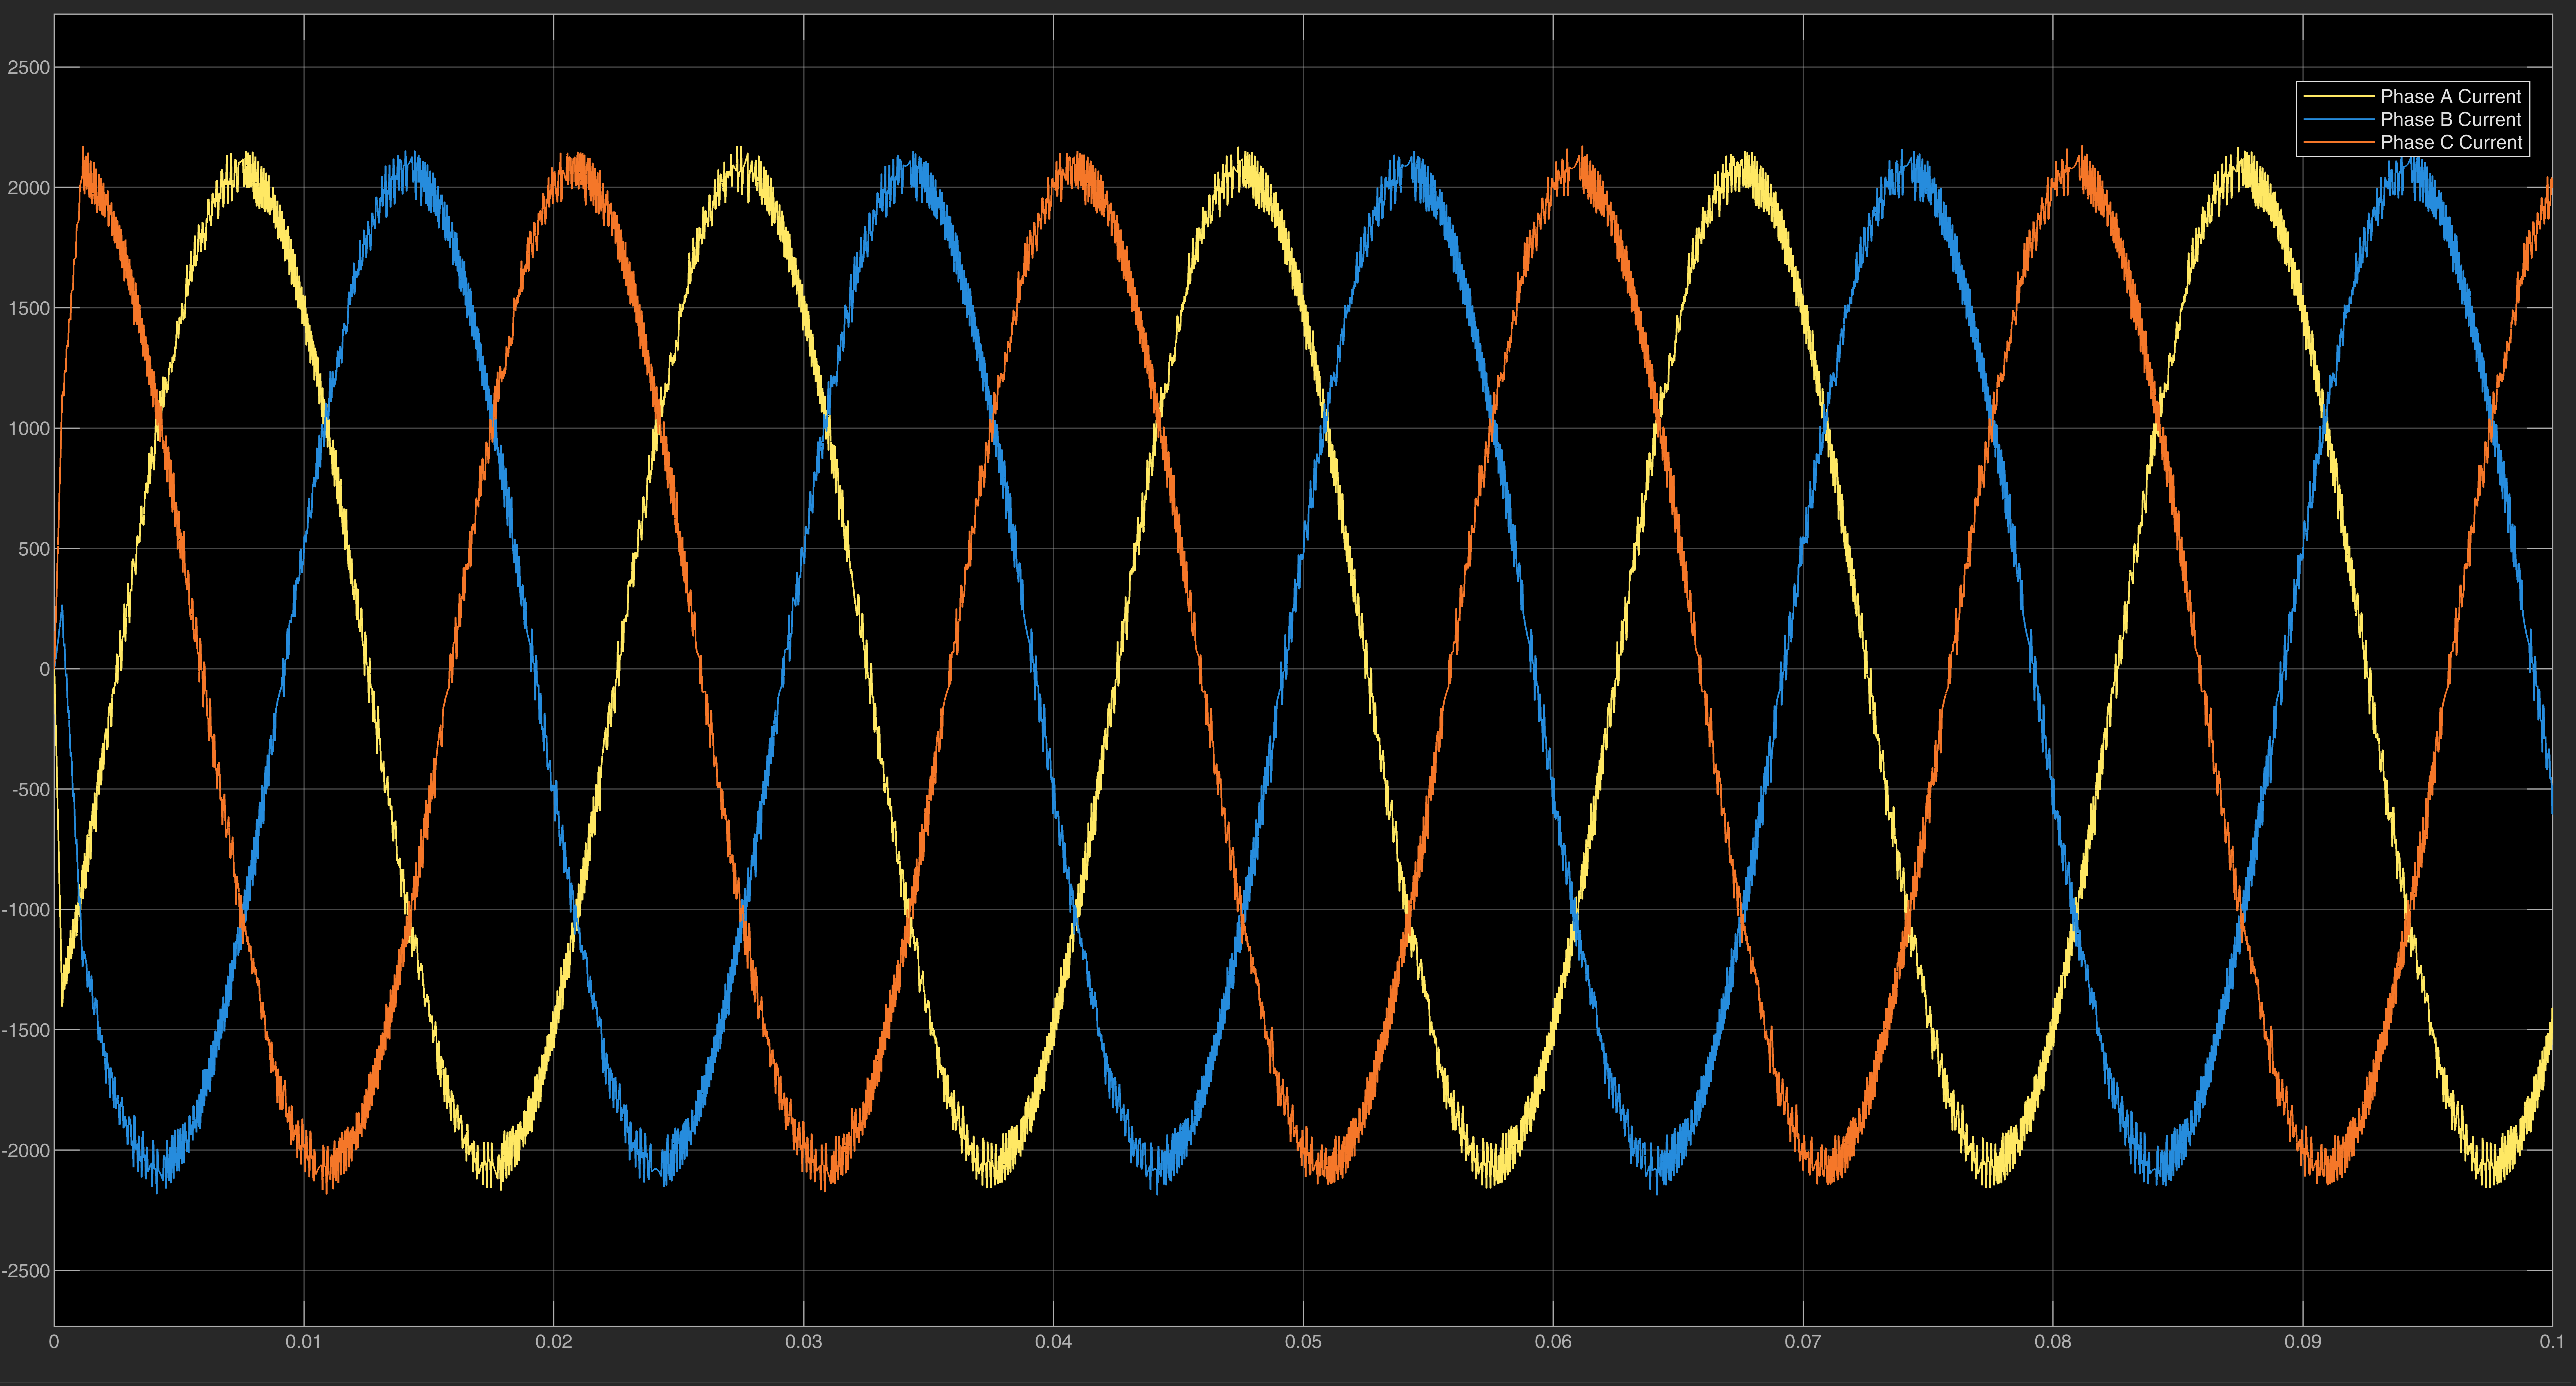
\includegraphics[width=\textwidth]{Grid Currents_2.png}
        \caption{Grid Currents}
    \end{subfigure}
    \vskip\baselineskip
    \begin{subfigure}{0.48\textwidth}
        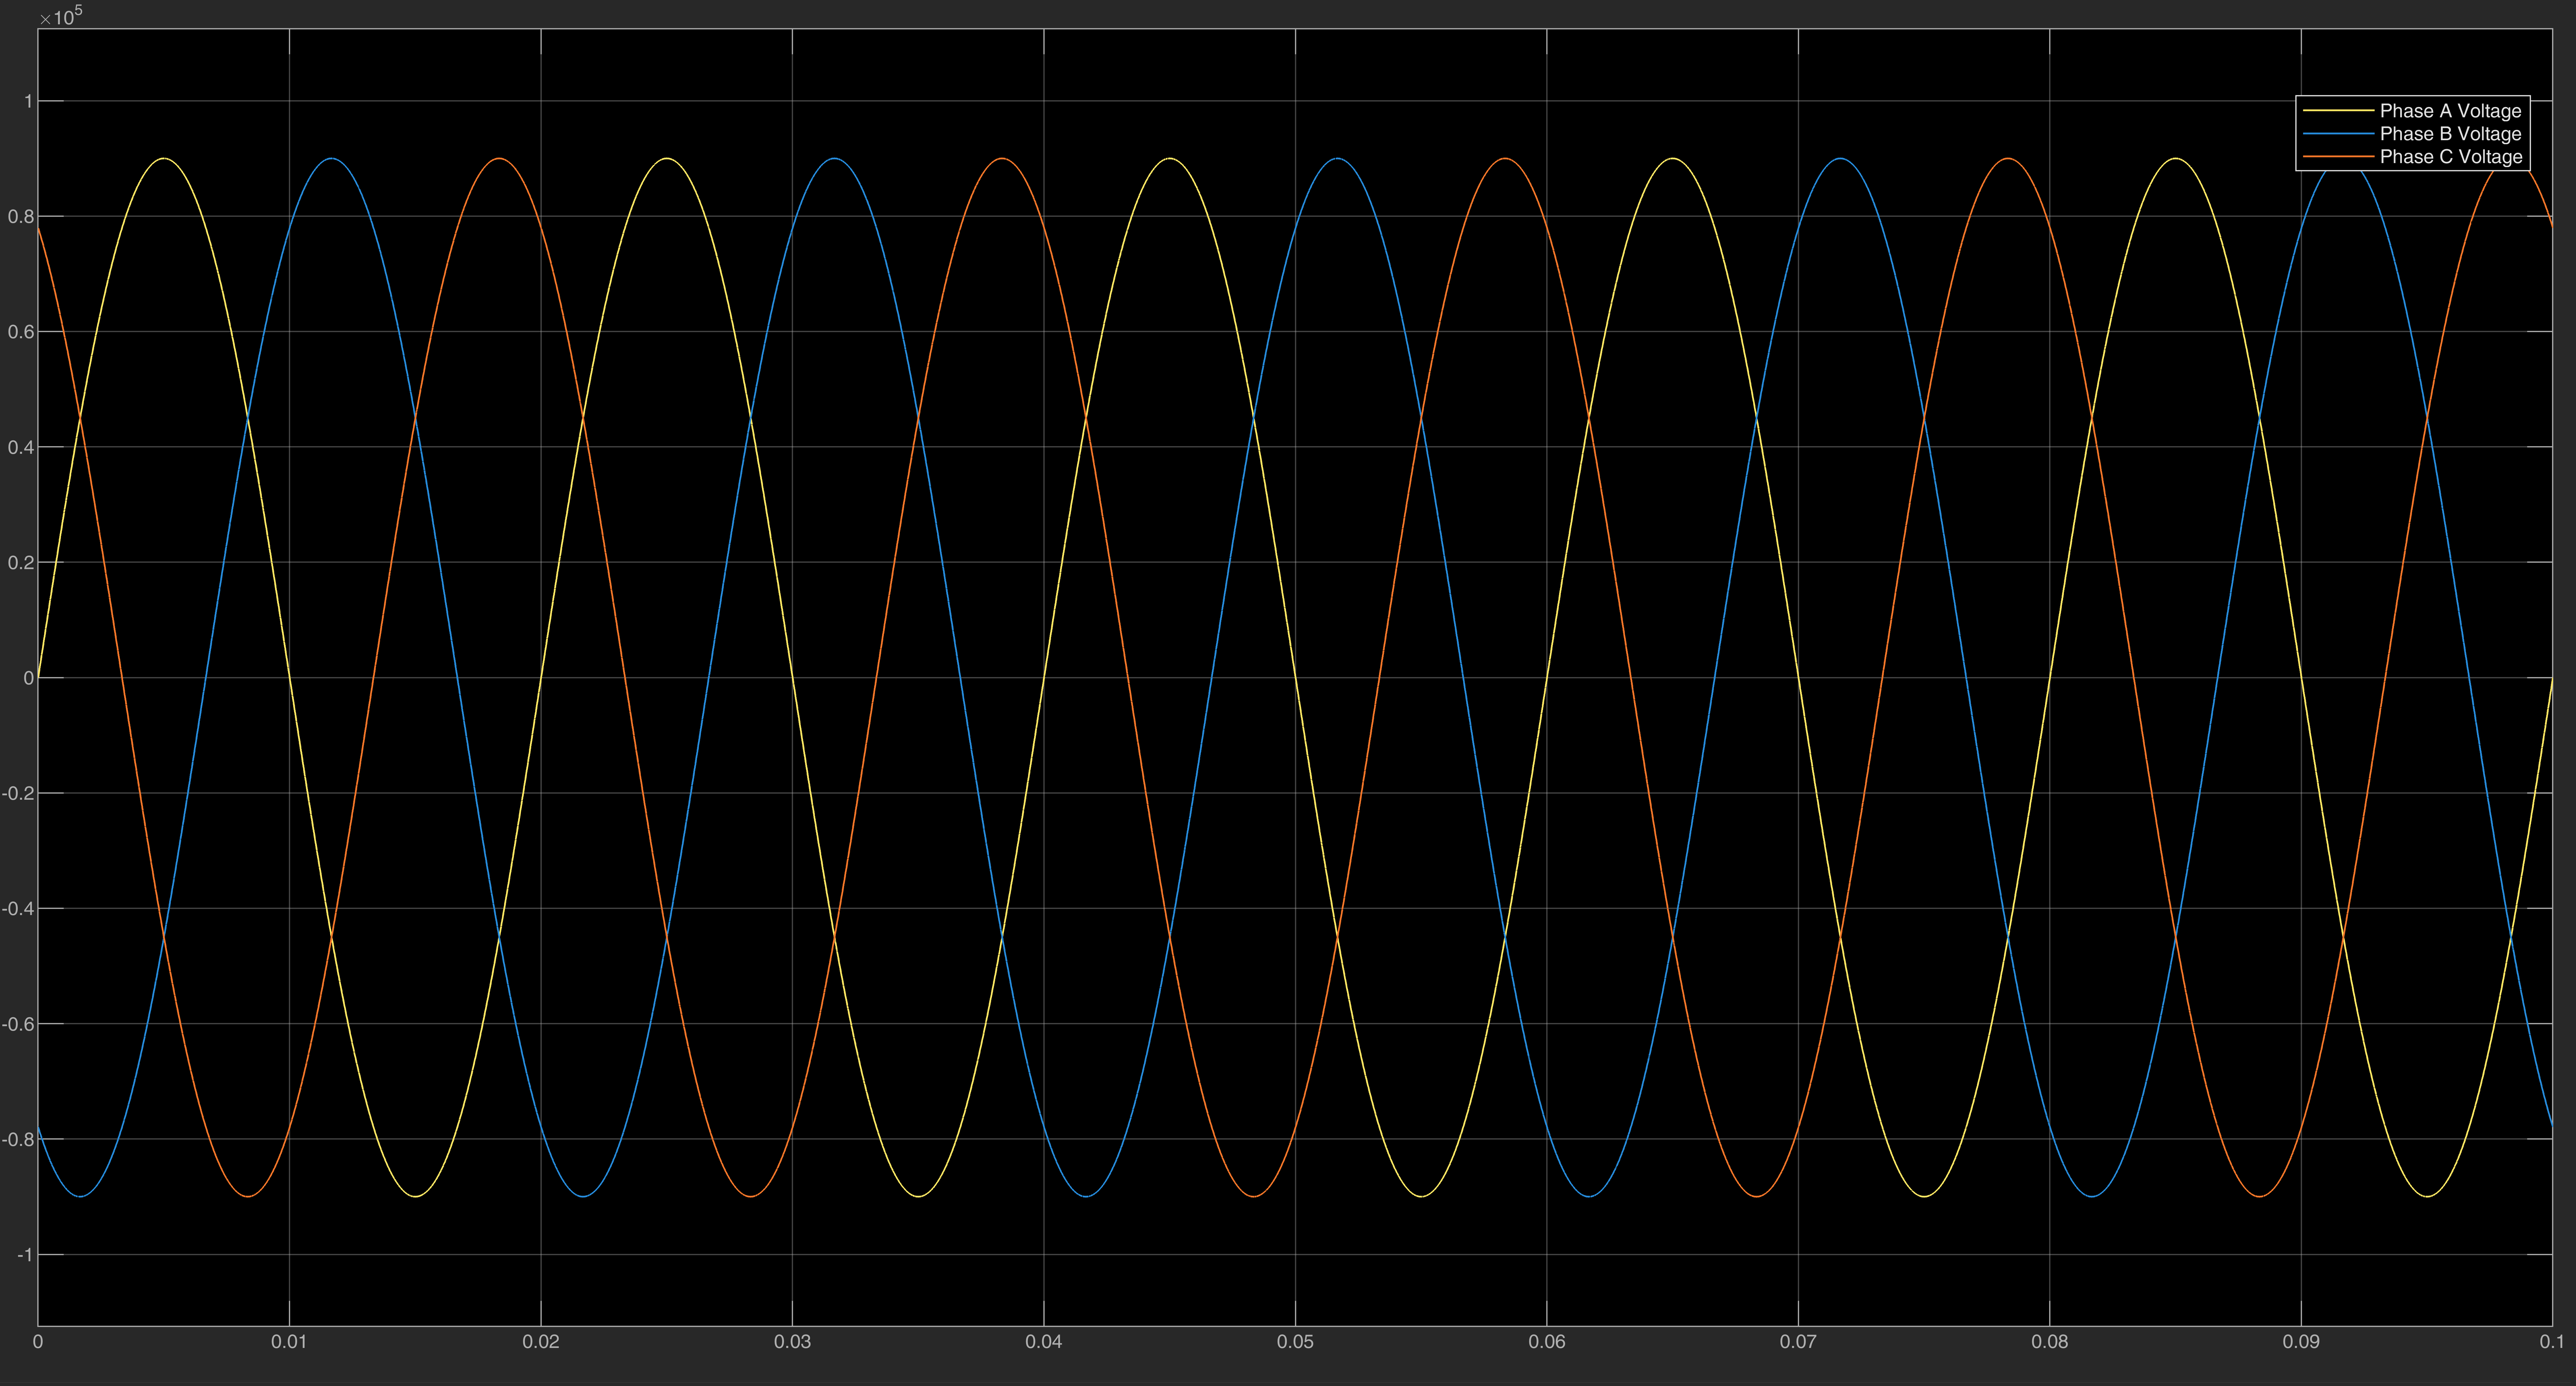
\includegraphics[width=\textwidth]{Grid Voltage_2.png}
        \caption{Grid Voltages}
    \end{subfigure}
    \hfill
    \begin{subfigure}{0.48\textwidth}
        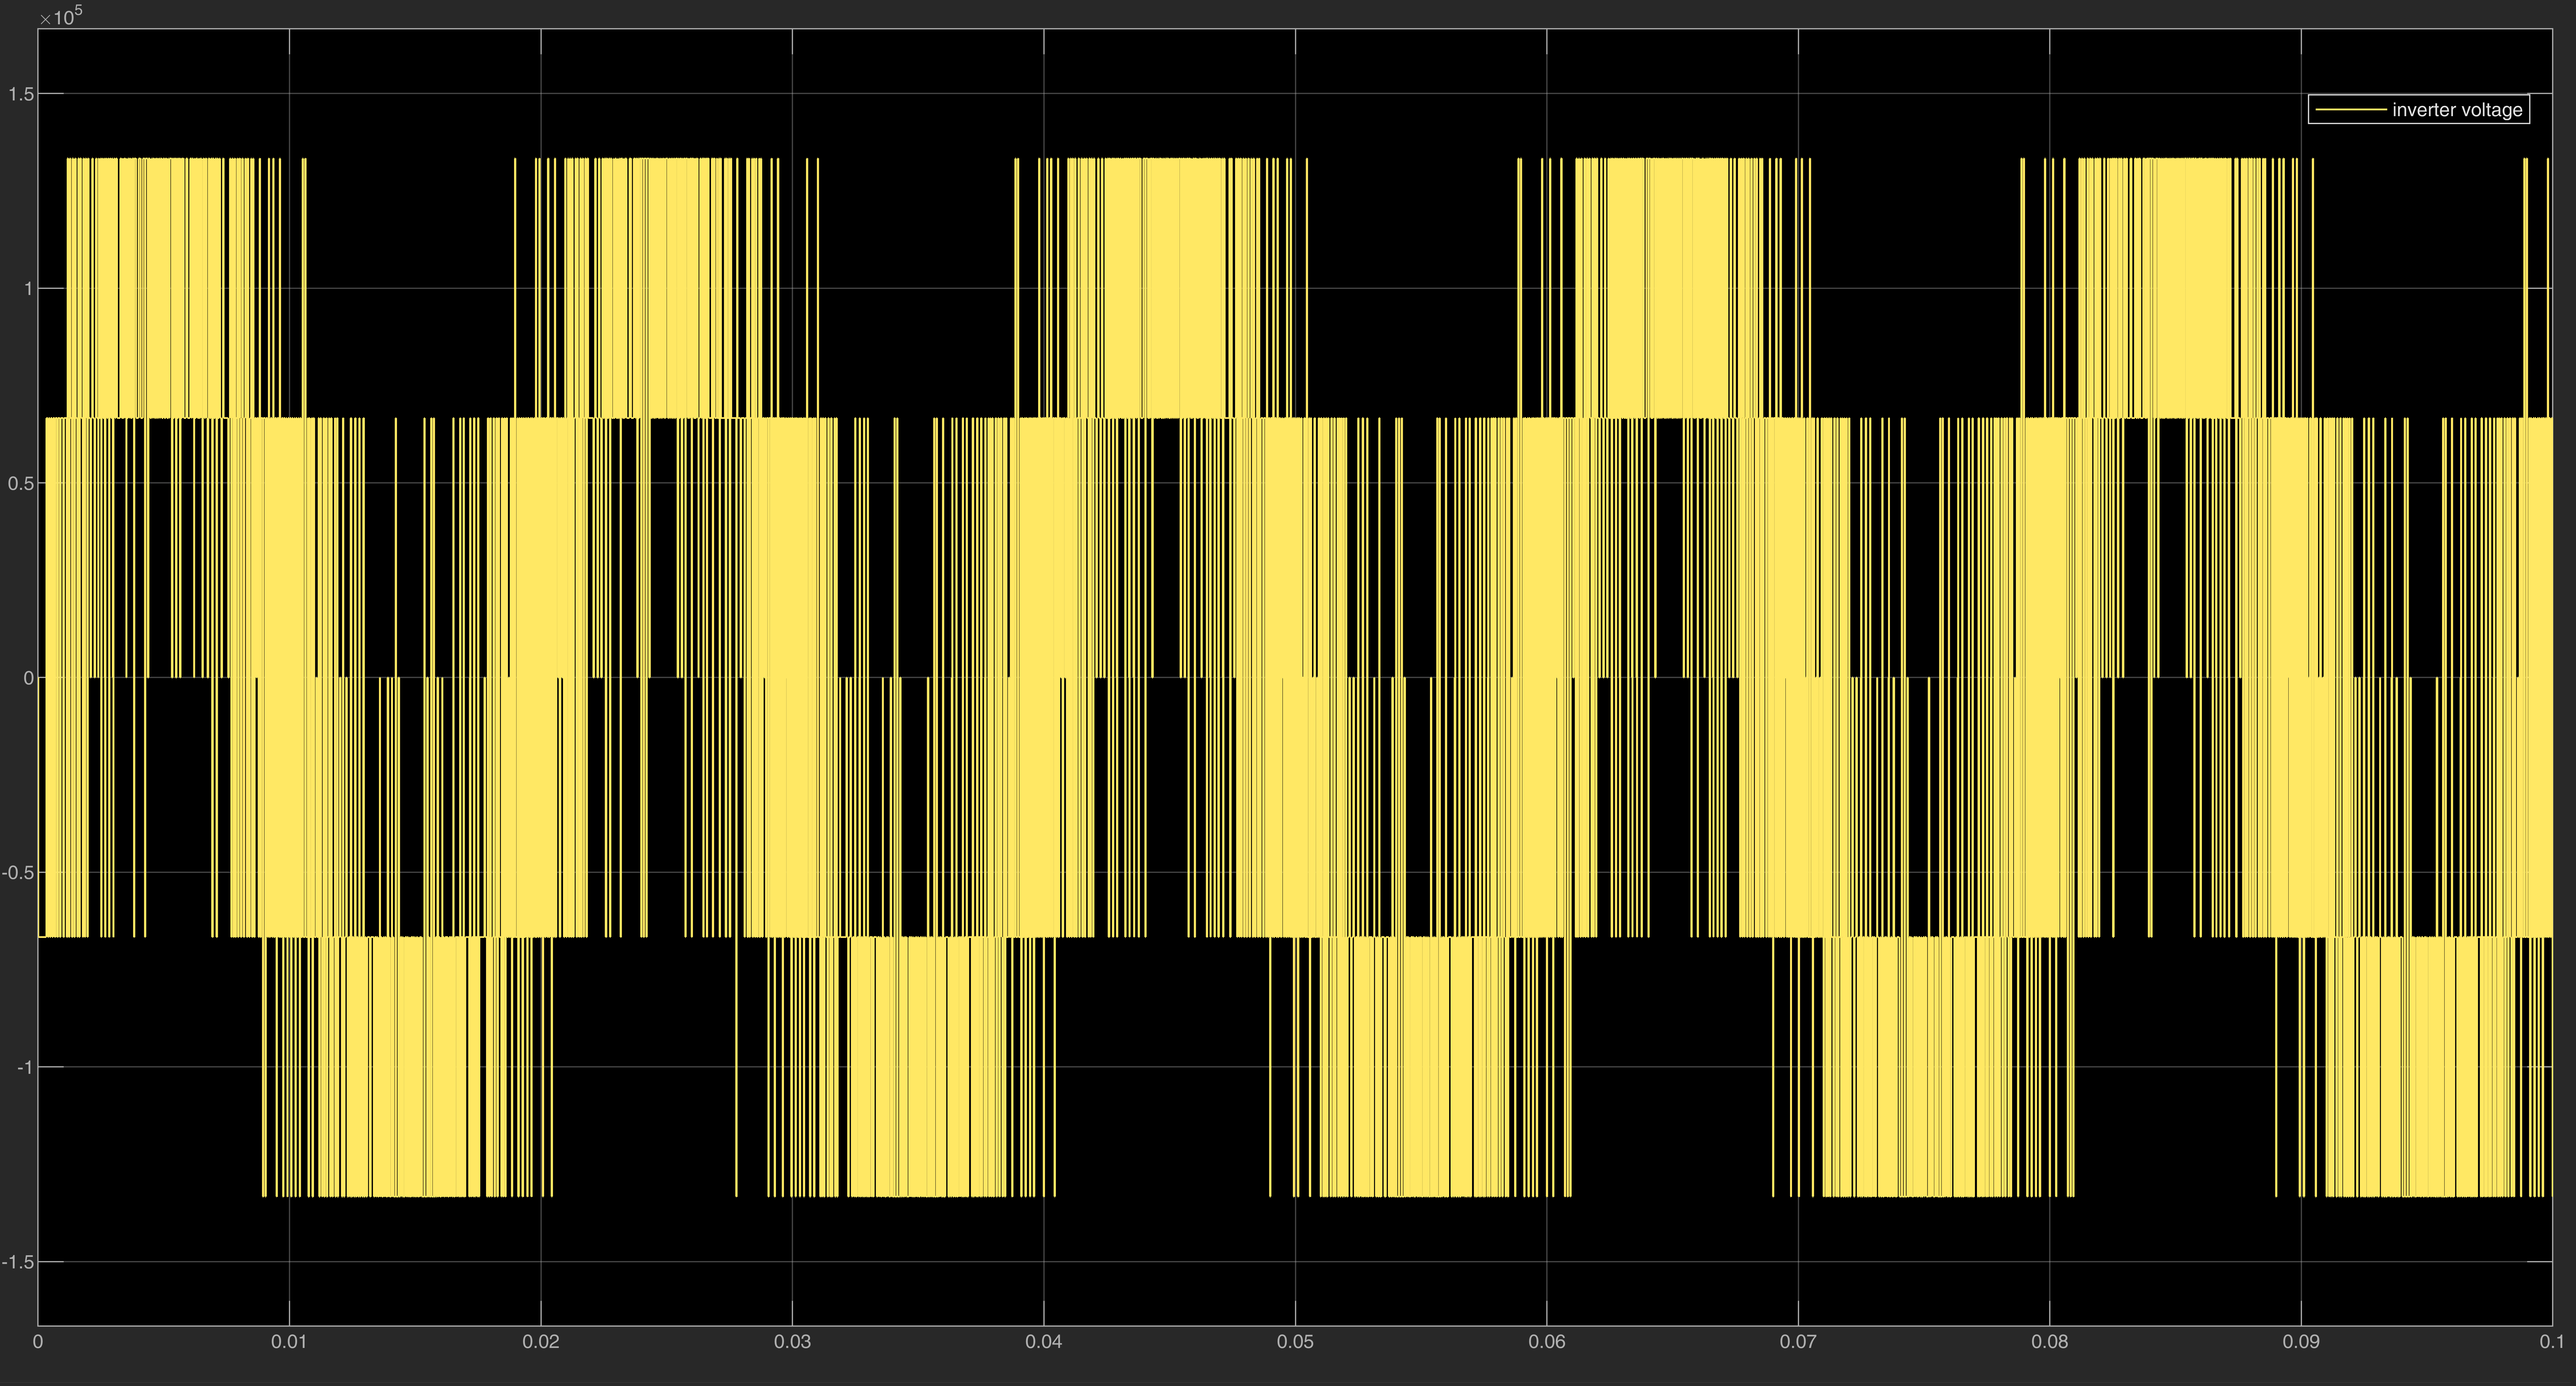
\includegraphics[width=\textwidth]{Inverter Phase Voltage_2.png}
        \caption{Inverter Phase Voltage}
    \end{subfigure}
    \caption{Simulation waveforms for Case 2 ($P=Q$ injection).}
\end{figure}

% --- Case 3 ---
\subsection{Case 3: Operation as STATCOM (0 MW, +405 MVAR)}
In this case, the active power reference is intentionally set to zero ($P = 0$), forcing the VSC to operate purely as a Static Synchronous Compensator (STATCOM). The converter injects maximum reactive power ($+405\text{ MVAR}$) into the AC network. This operation mode is highly beneficial in modern power systems for providing dynamic voltage regulation and compensating heavily loaded inductive transmission lines.

The absence of active power transfer is physically evident in the waveforms, as the grid currents are shifted exactly $90^\circ$ (leading/lagging) relative to the phase voltages. During this mode, the DC link capacitor theoretically exchanges no net active power with the AC grid (ignoring internal switching losses and filter resistance). The controller successfully enforces the zero active power condition while strictly maintaining the $405\text{ MVAR}$ reactive power injection.

\begin{figure}[H]
    \centering
    \begin{subfigure}{0.48\textwidth}
        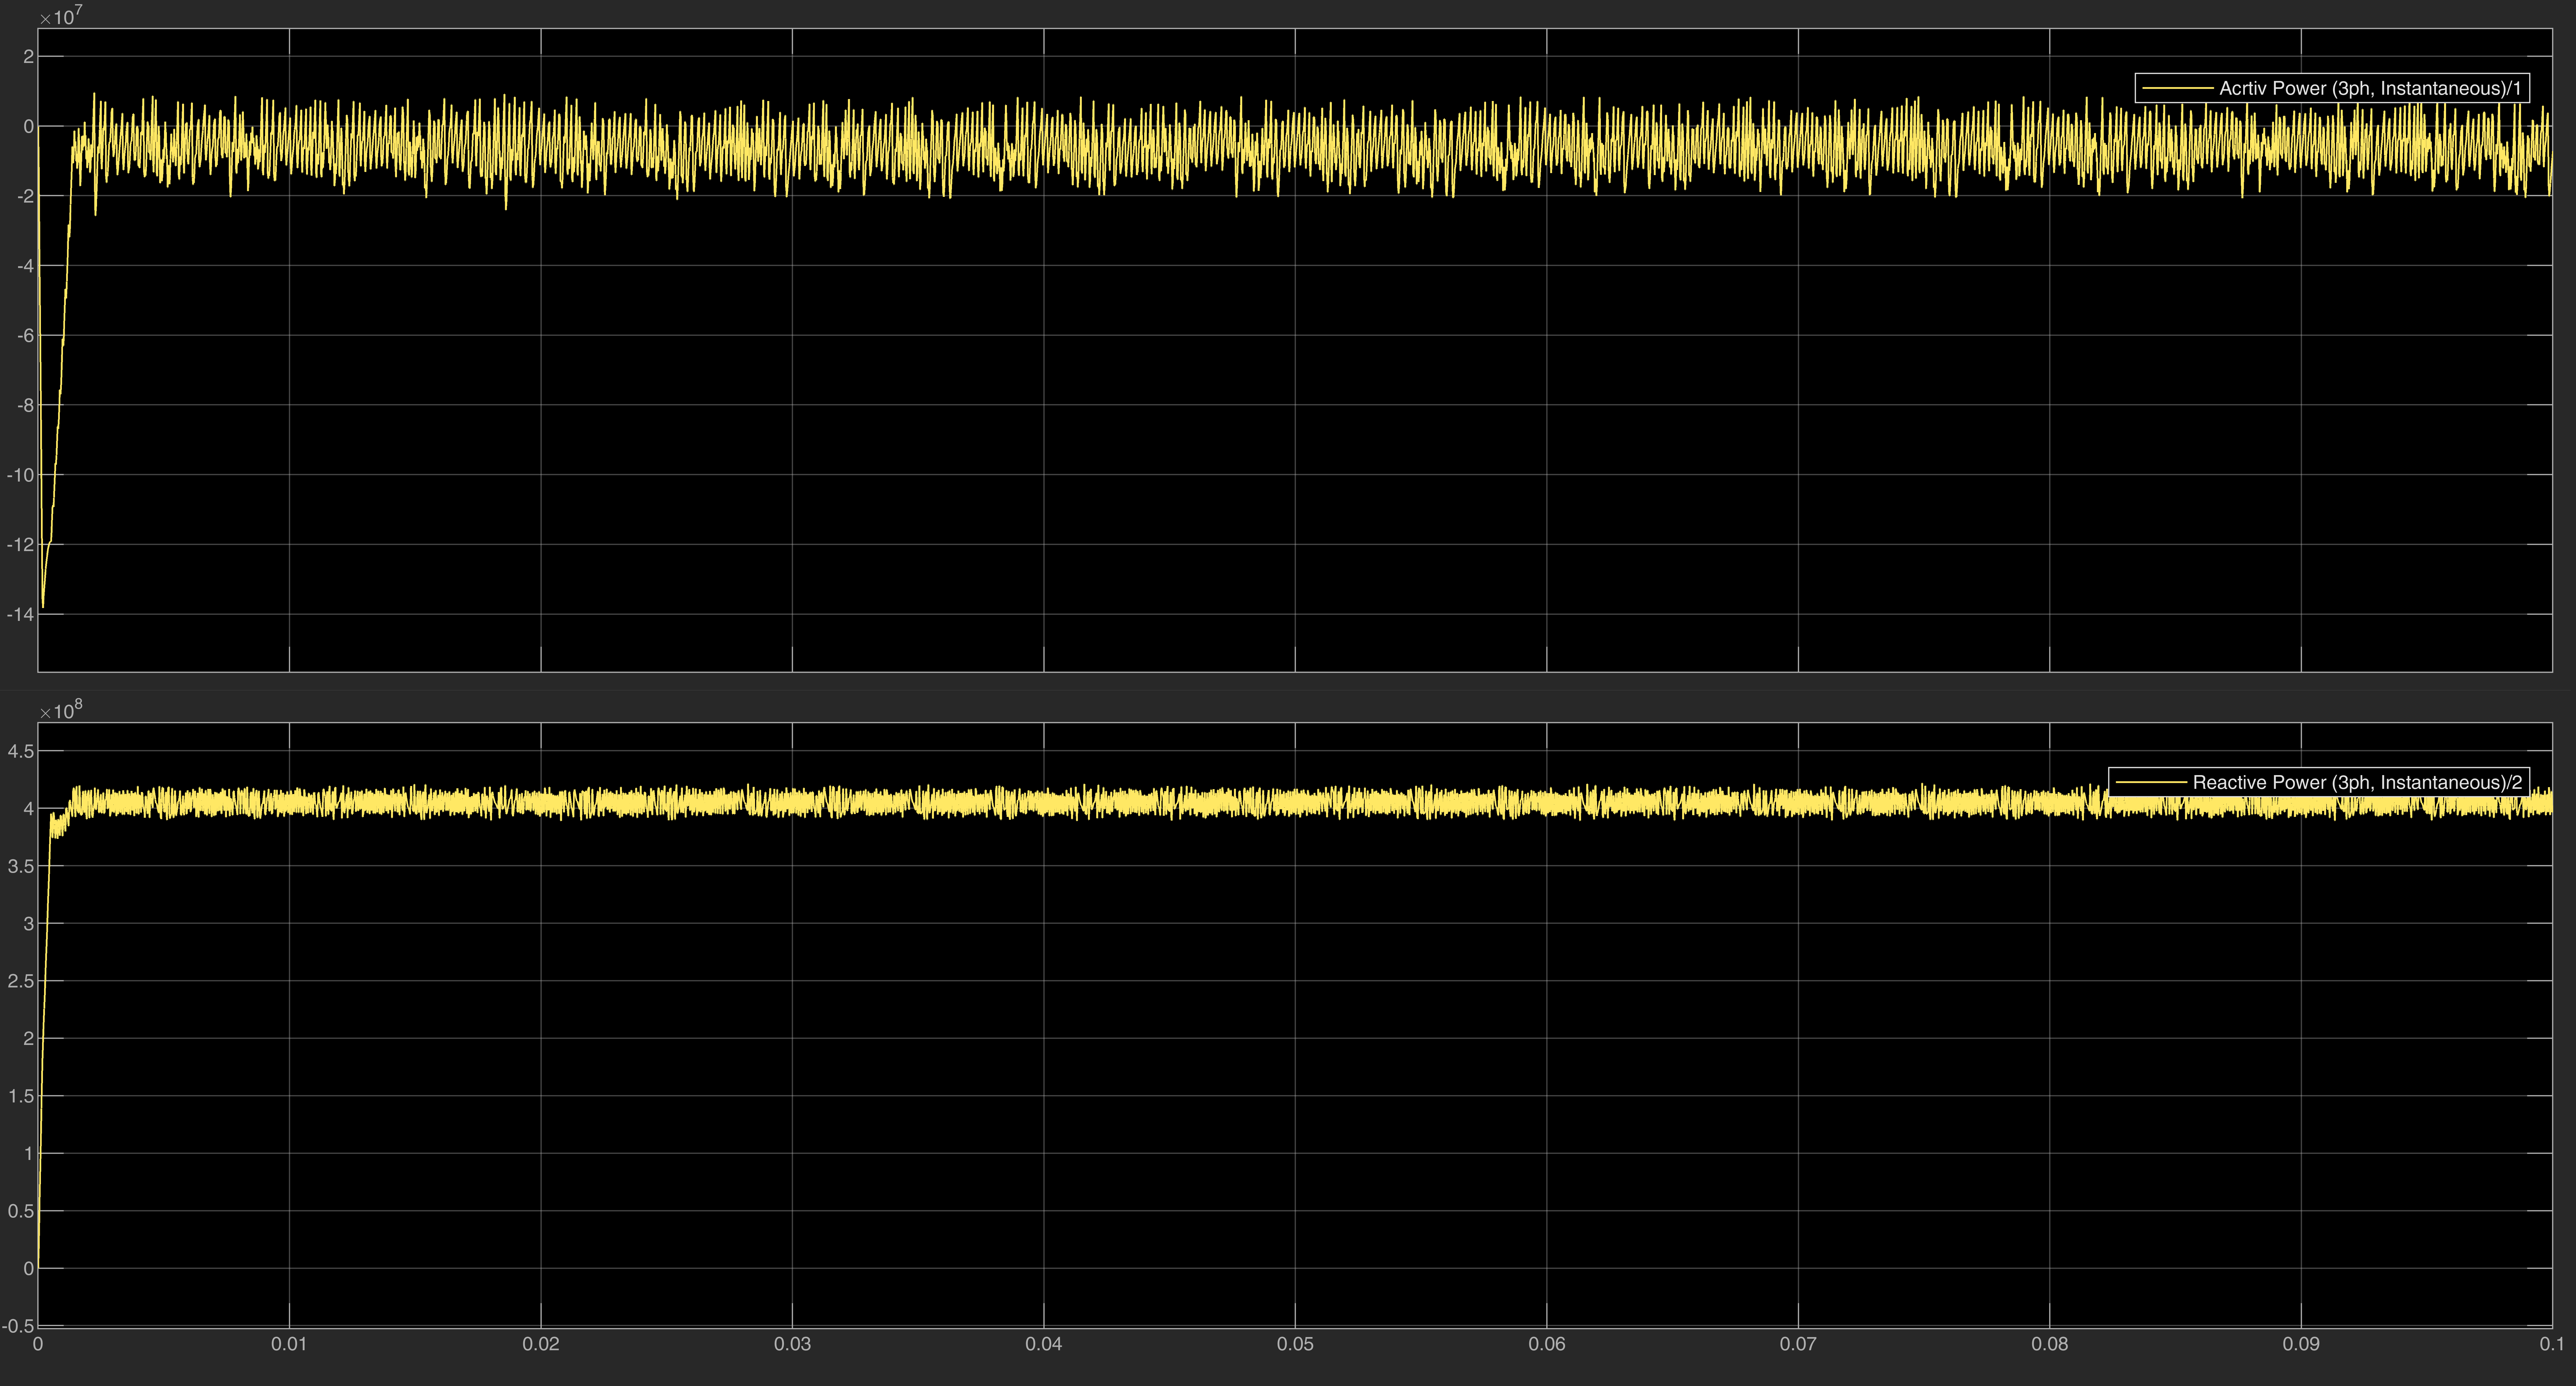
\includegraphics[width=\textwidth]{Grid active and reactive powers_3.png}
        \caption{Active and Reactive Power}
    \end{subfigure}
    \hfill
    \begin{subfigure}{0.48\textwidth}
        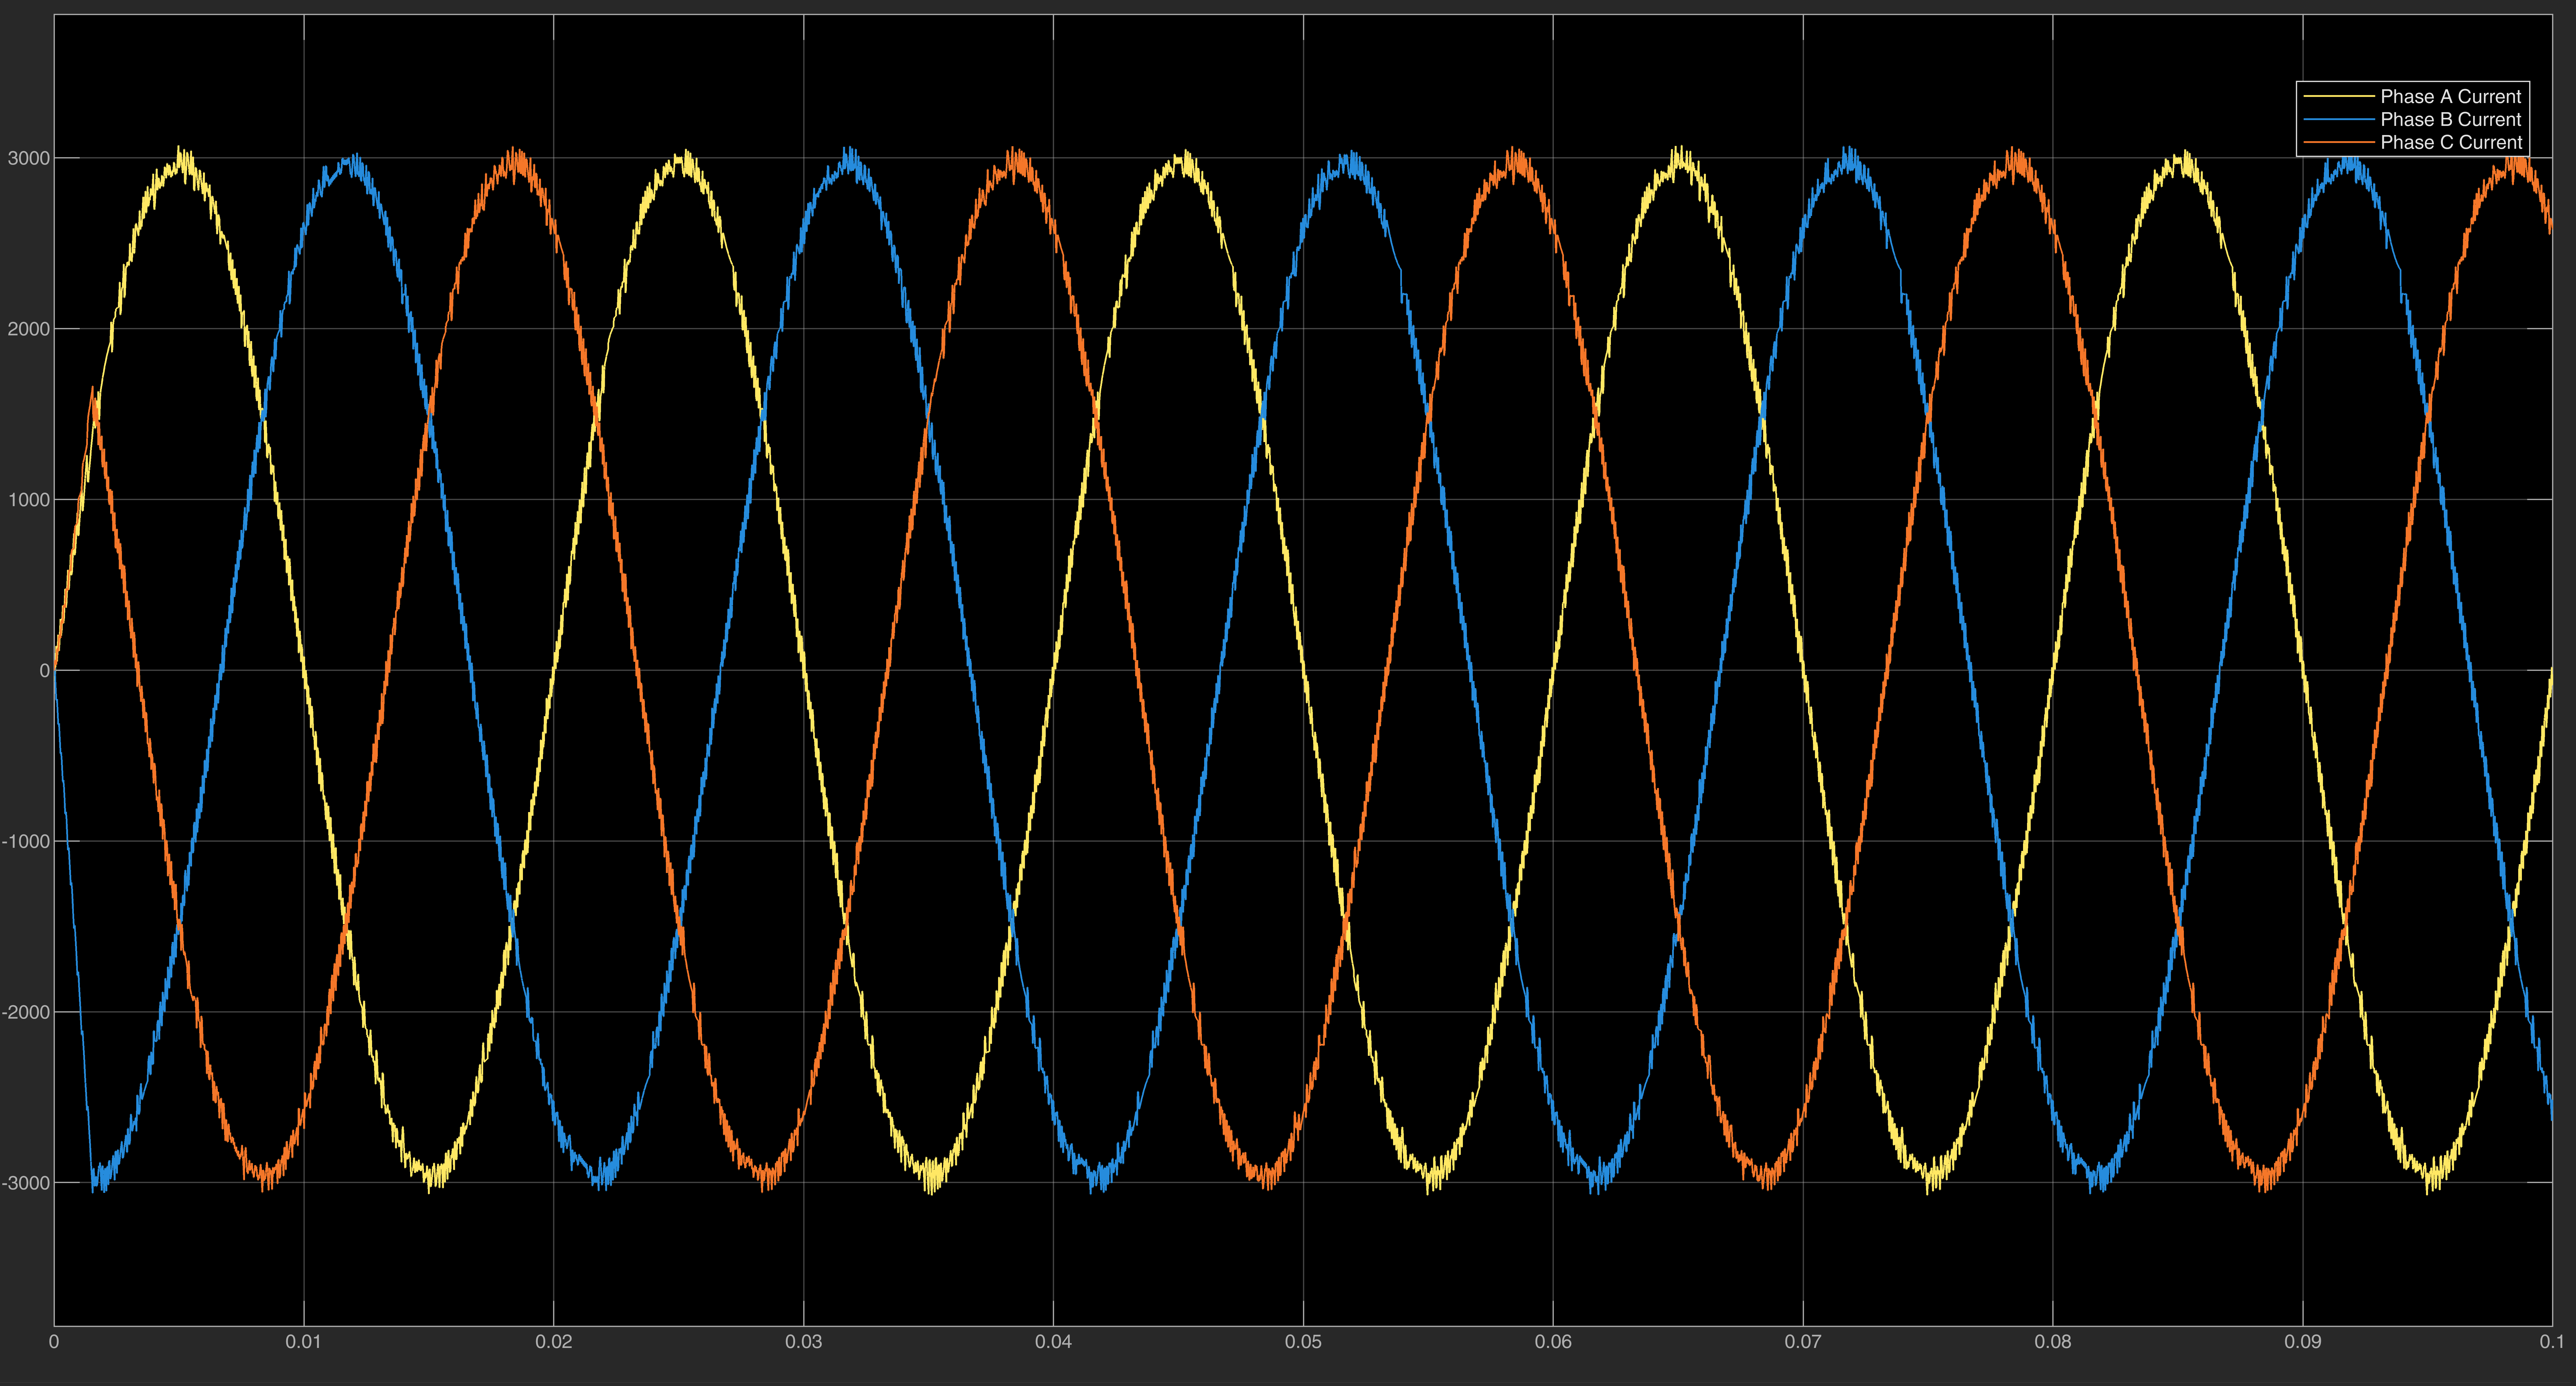
\includegraphics[width=\textwidth]{Grid Currents_3.png}
        \caption{Grid Currents}
    \end{subfigure}
    \vskip\baselineskip
    \begin{subfigure}{0.48\textwidth}
        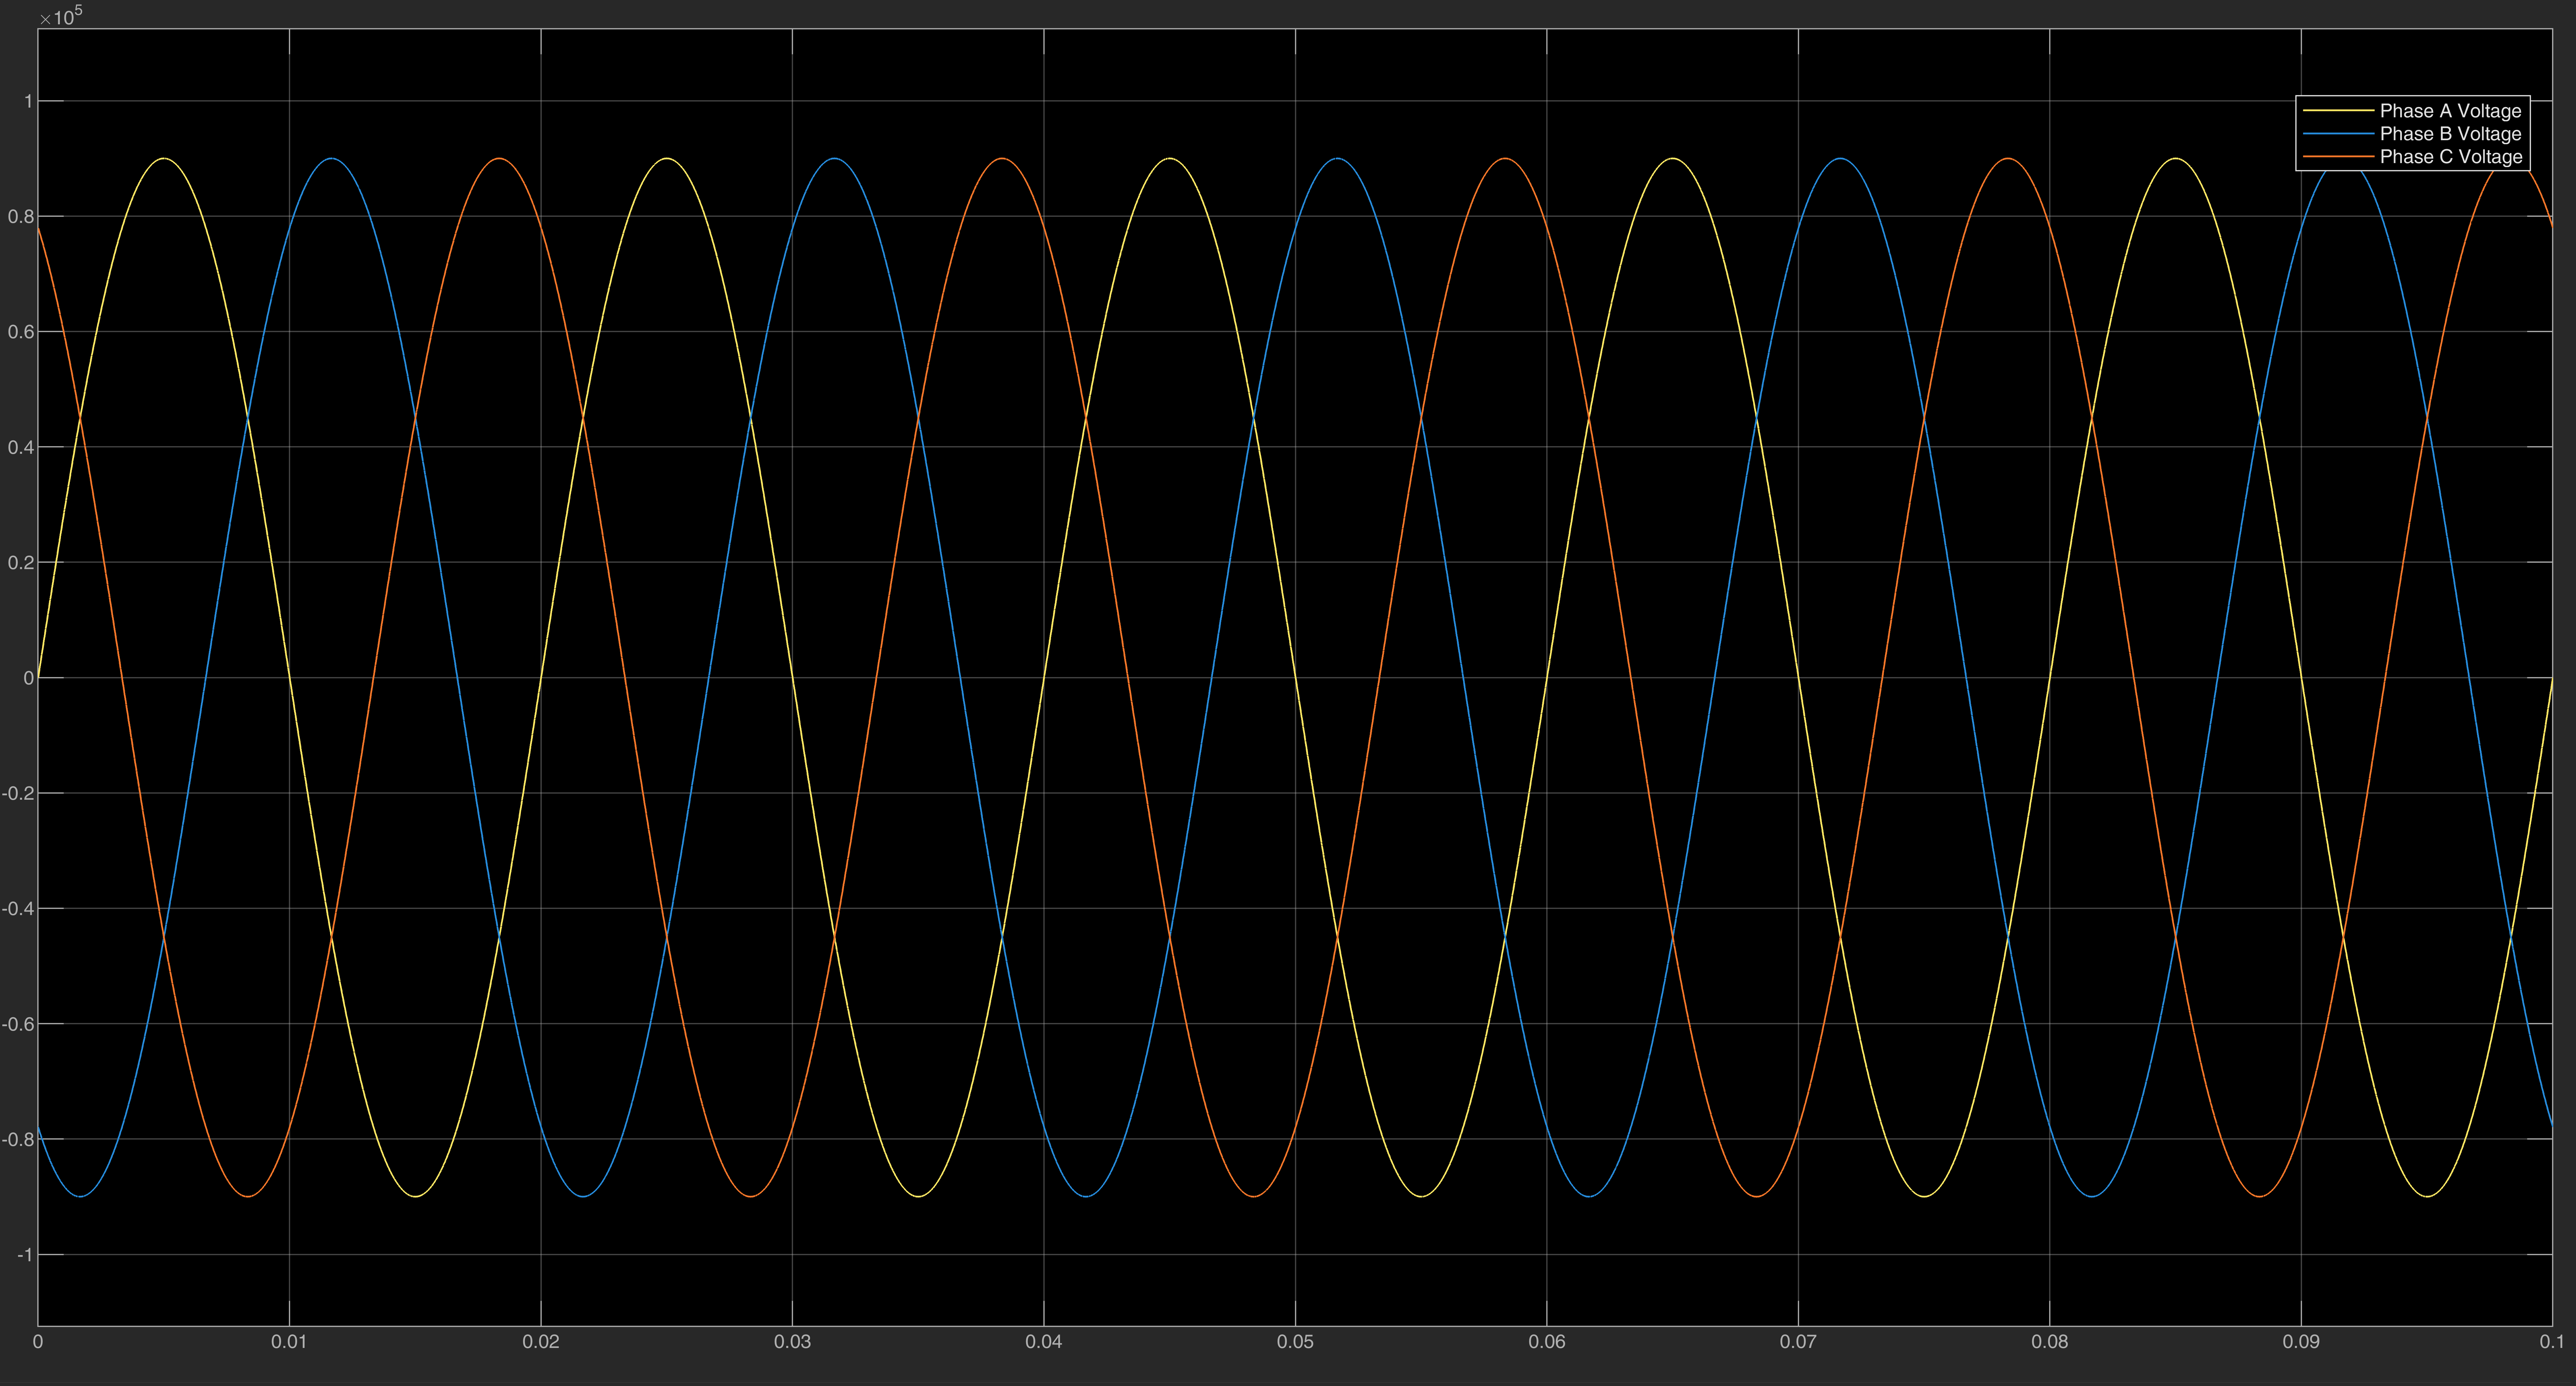
\includegraphics[width=\textwidth]{Grid Voltage_3.png}
        \caption{Grid Voltages}
    \end{subfigure}
    \hfill
    \begin{subfigure}{0.48\textwidth}
        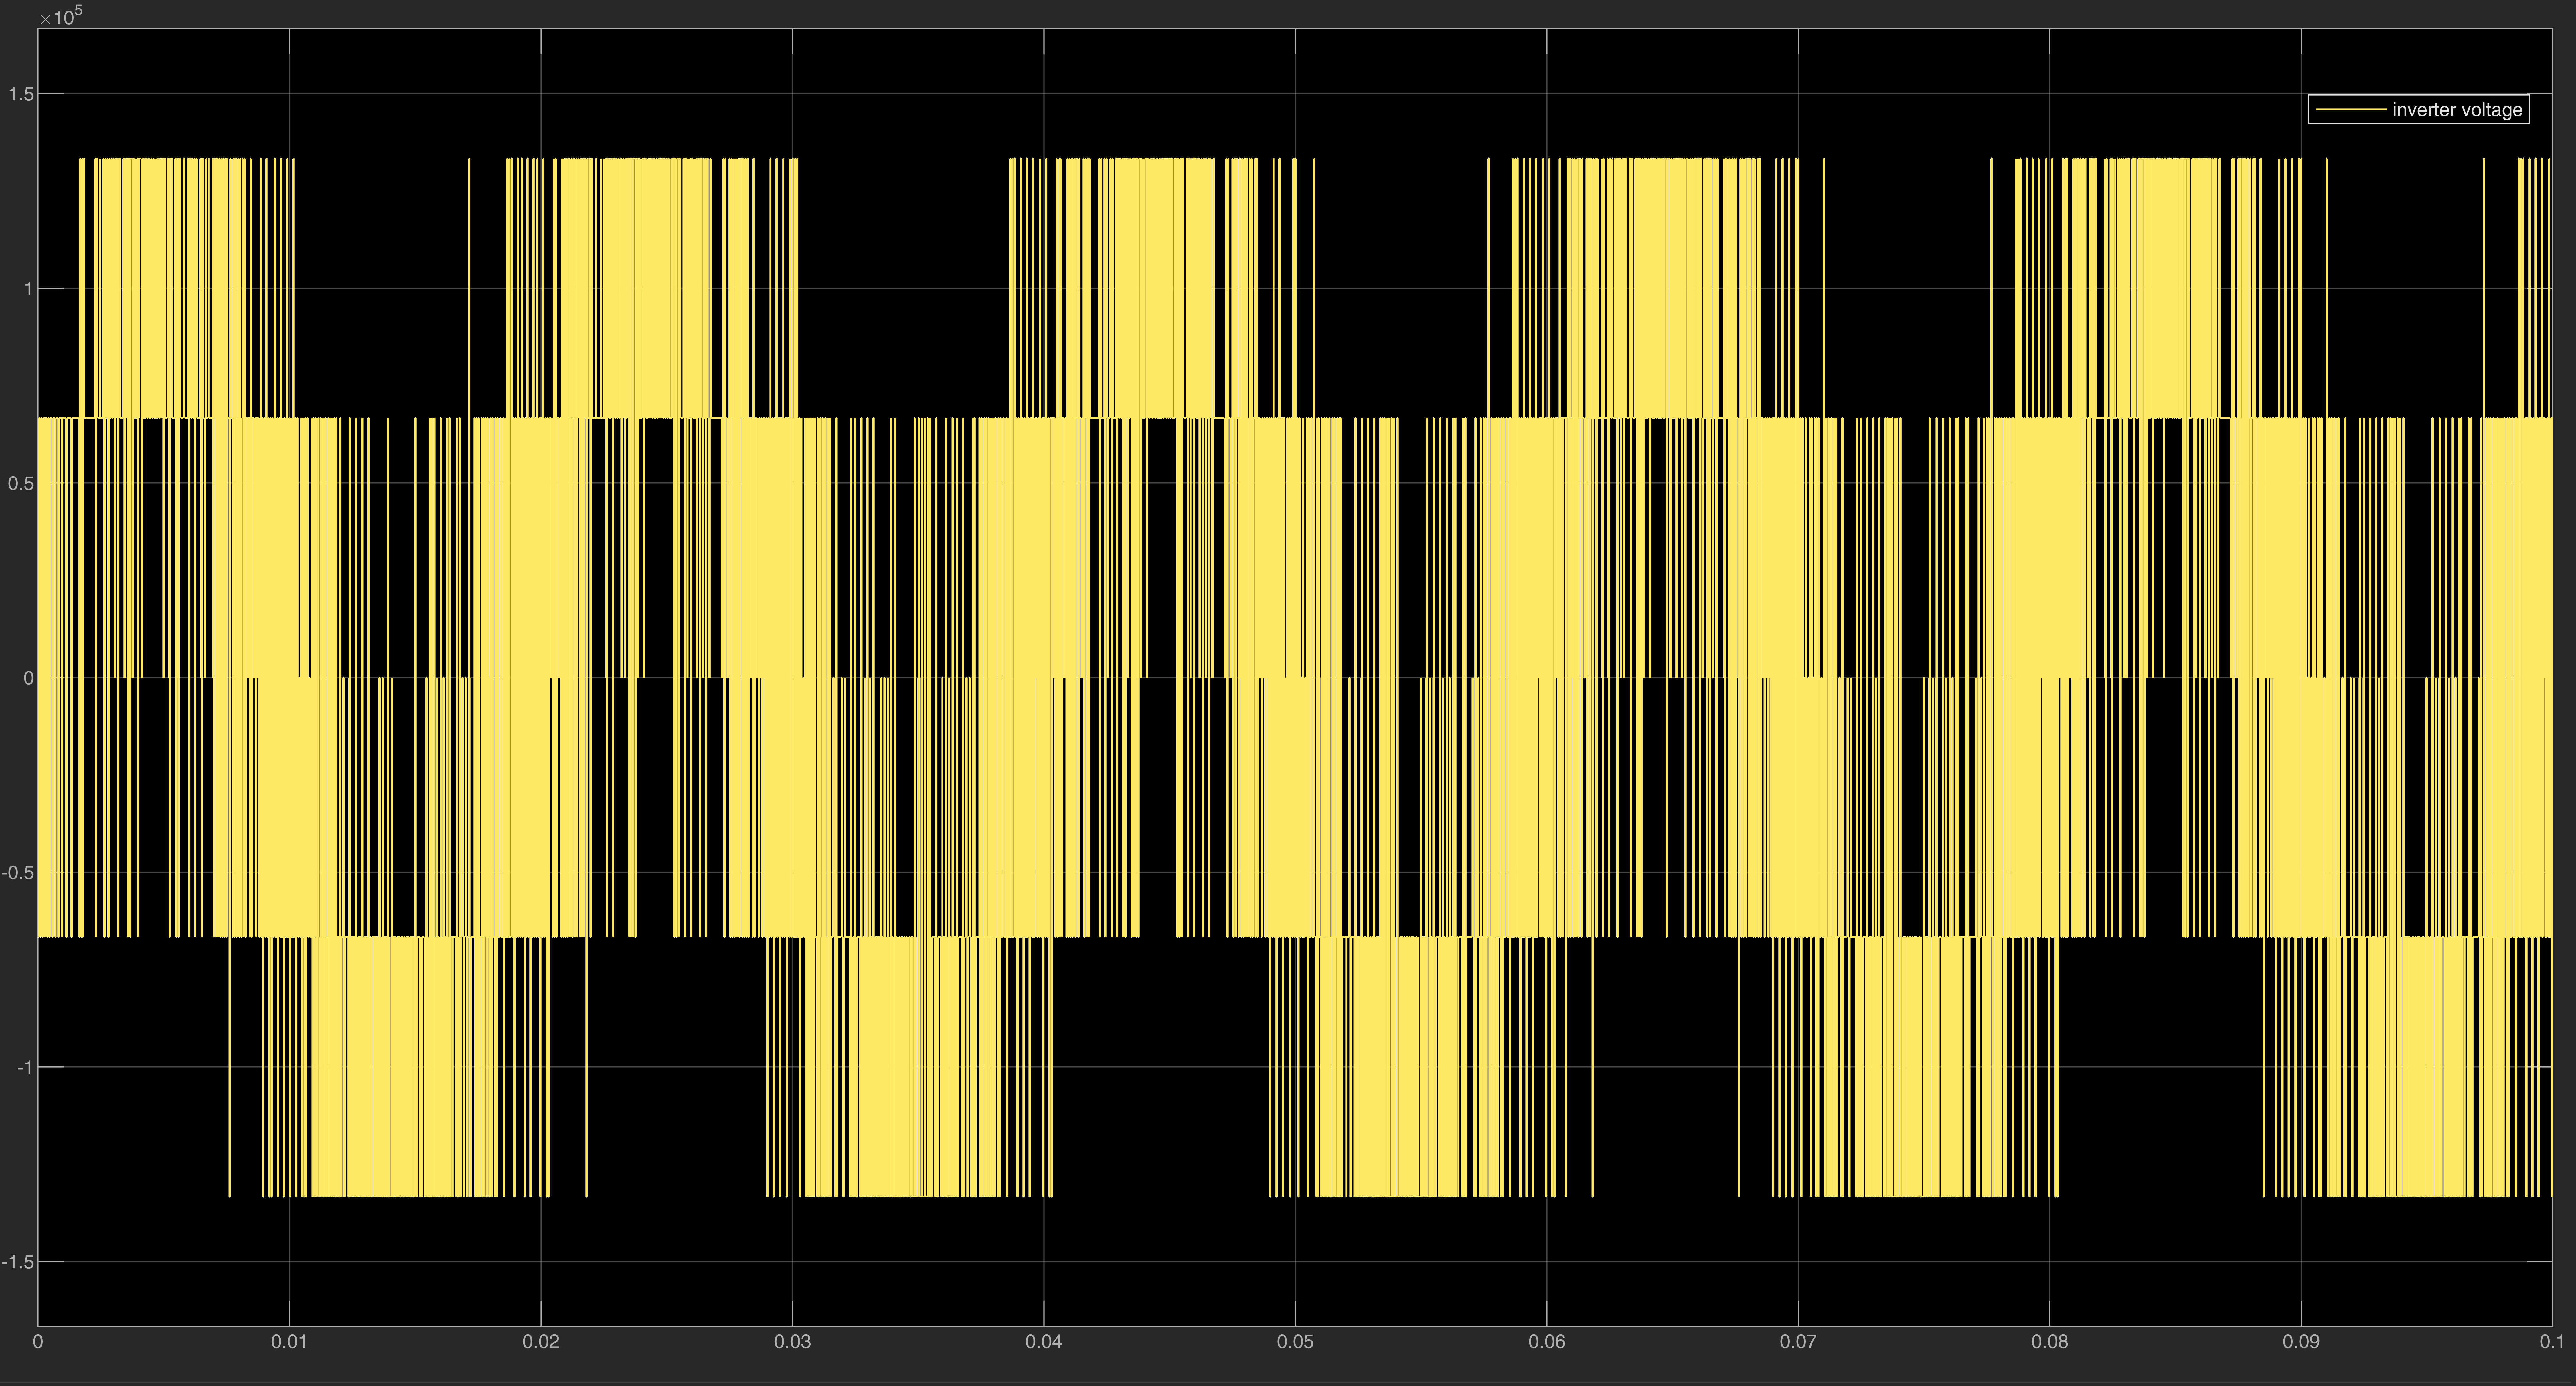
\includegraphics[width=\textwidth]{Inverter Phase Voltage_3.png}
        \caption{Inverter Phase Voltage}
    \end{subfigure}
    \caption{Simulation waveforms for Case 3 (STATCOM Mode).}
\end{figure}

% --- Case 4 ---
\subsection{Case 4: Negative Active Power Flow (-405 MW, 0 MVAR)}
This scenario tests the bidirectional power flow capability of the VSC, a crucial feature for multi-terminal HVDC grids and regenerative braking applications. With a negative active power reference ($P = -405\text{ MW}$), the converter transitions into rectification mode, drawing active power from the AC grid and delivering it to the DC side. 

The magnitude of the current remains constant at $3000\text{ A}$ since the absolute apparent power requirement is unchanged from Case 1. However, the waveforms reveal the underlying mechanism of power reversal: a complete $180^\circ$ phase shift. The grid currents are now operating in anti-phase relative to the grid voltages. This $180^\circ$ shift is successfully executed by the controller while keeping the reactive power strictly regulated at zero.

\begin{figure}[H]
    \centering
    \begin{subfigure}{0.48\textwidth}
        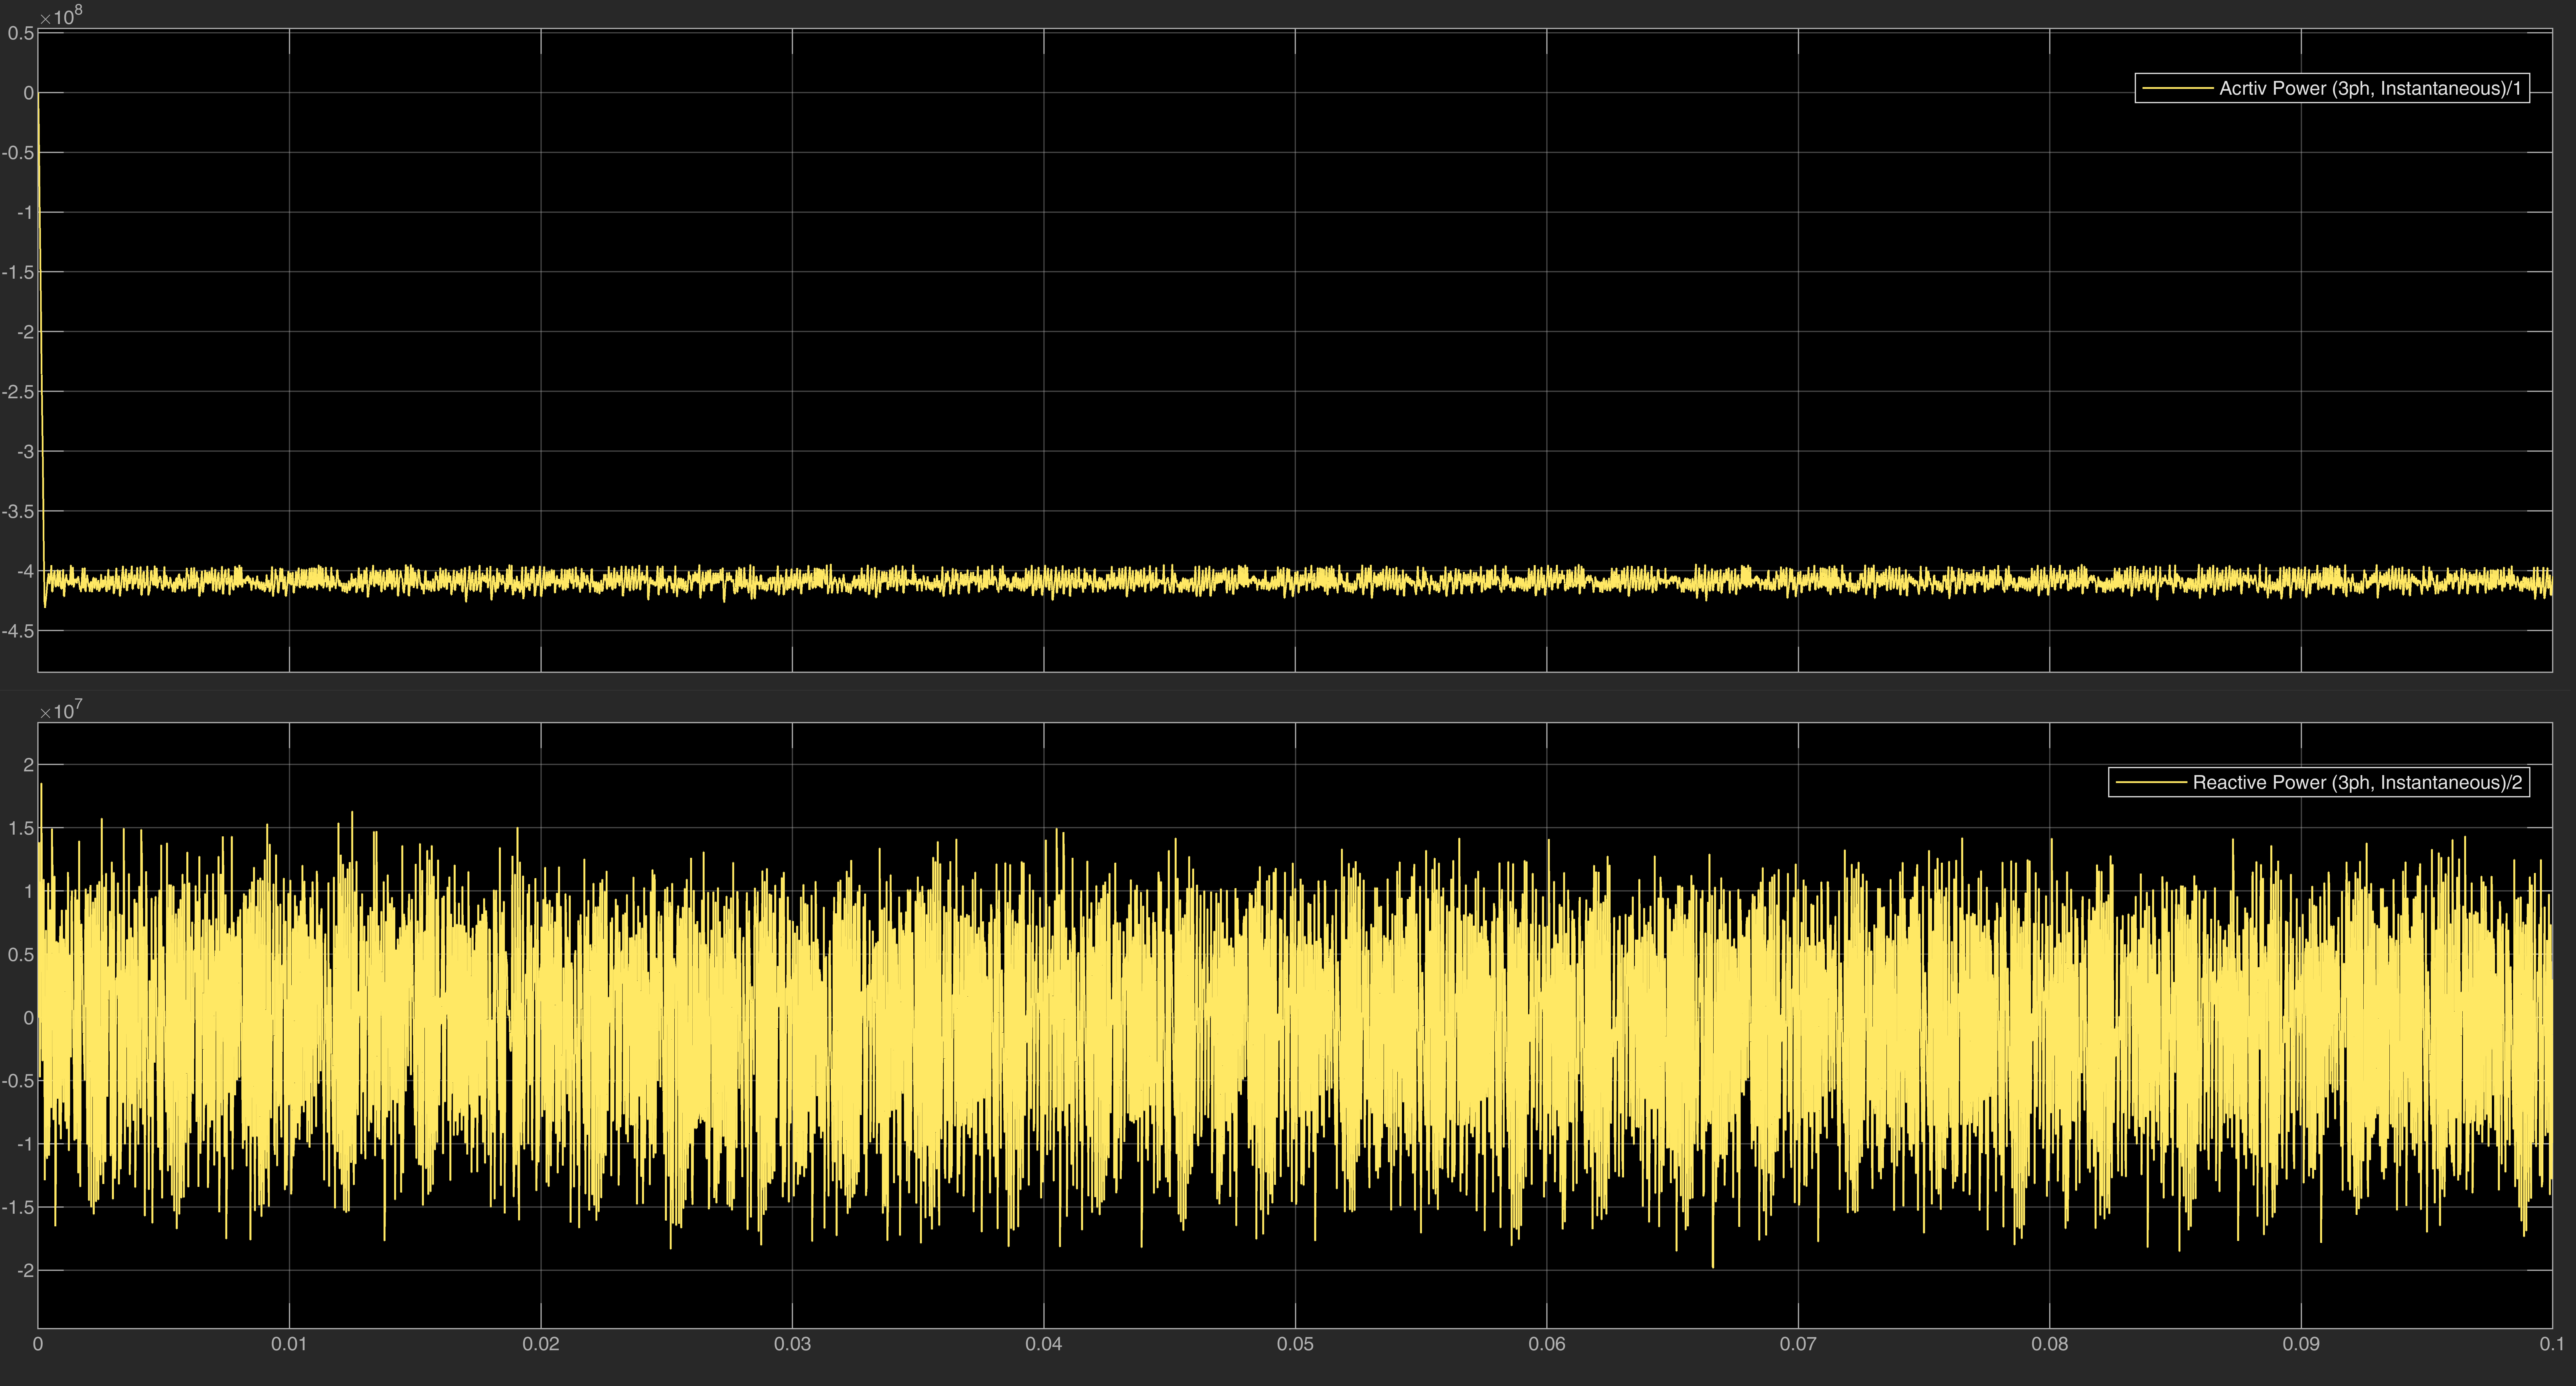
\includegraphics[width=\textwidth]{Grid active and reactive powers_4.png}
        \caption{Active and Reactive Power}
    \end{subfigure}
    \hfill
    \begin{subfigure}{0.48\textwidth}
        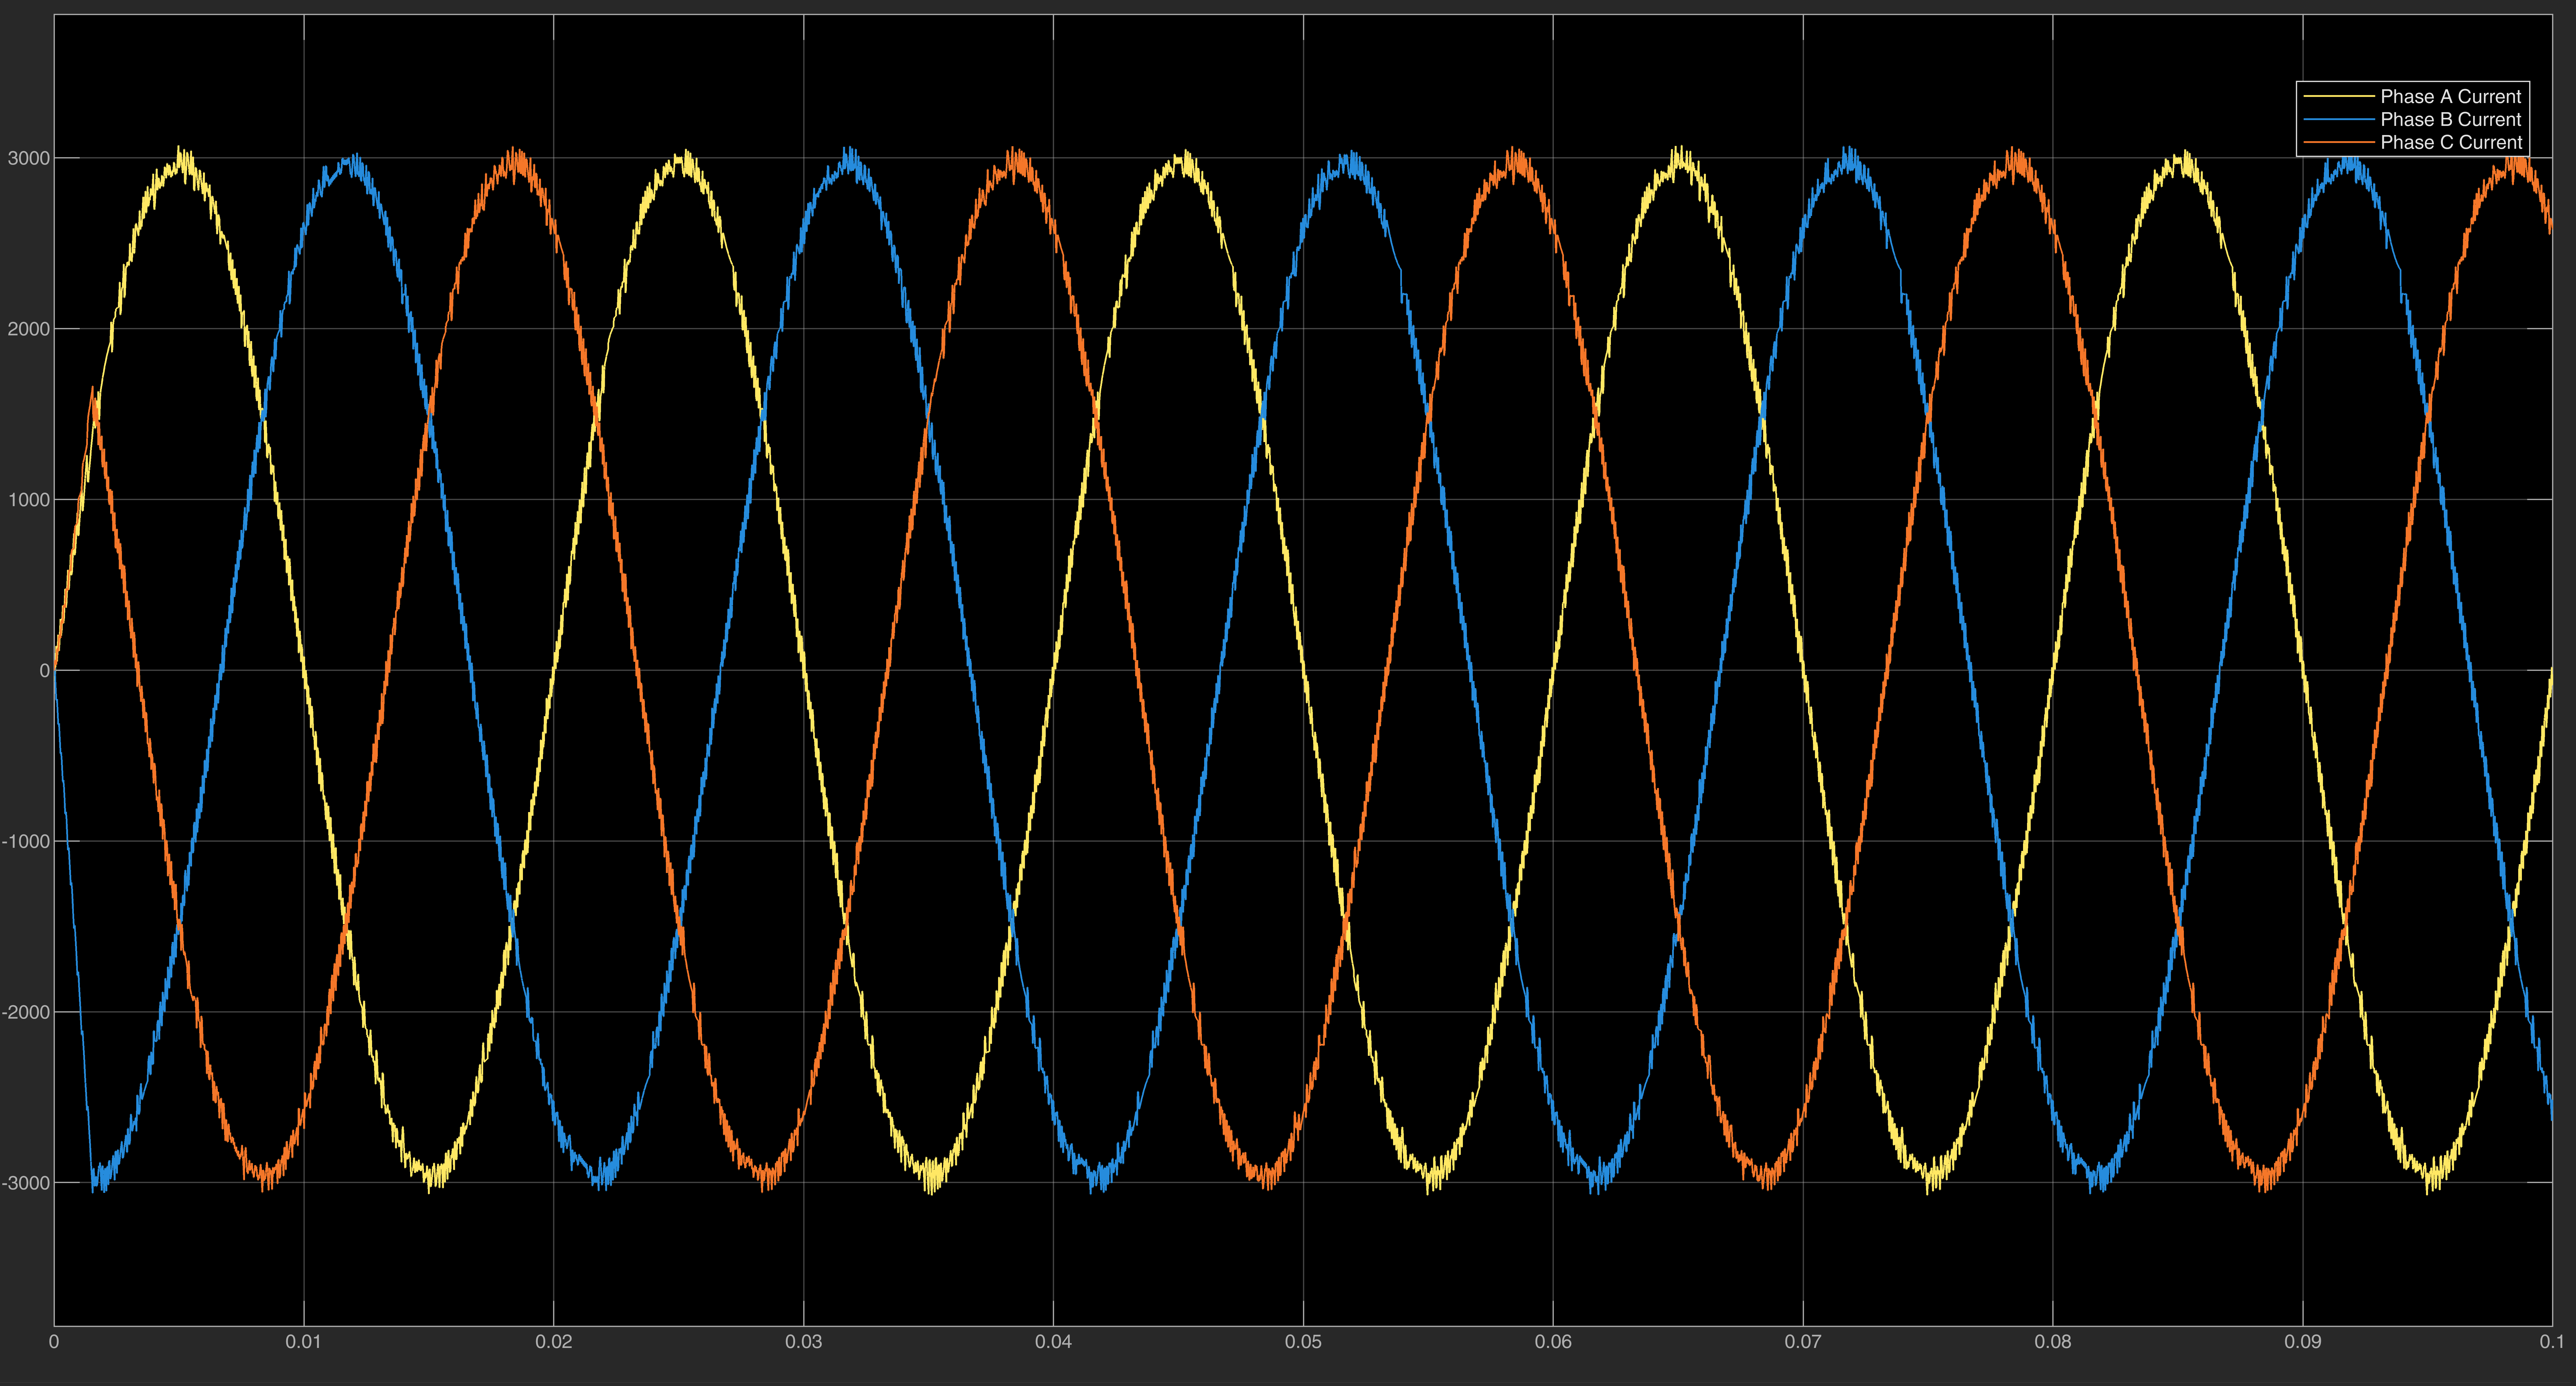
\includegraphics[width=\textwidth]{Grid Currents_4.png}
        \caption{Grid Currents}
    \end{subfigure}
    \vskip\baselineskip
    \begin{subfigure}{0.48\textwidth}
        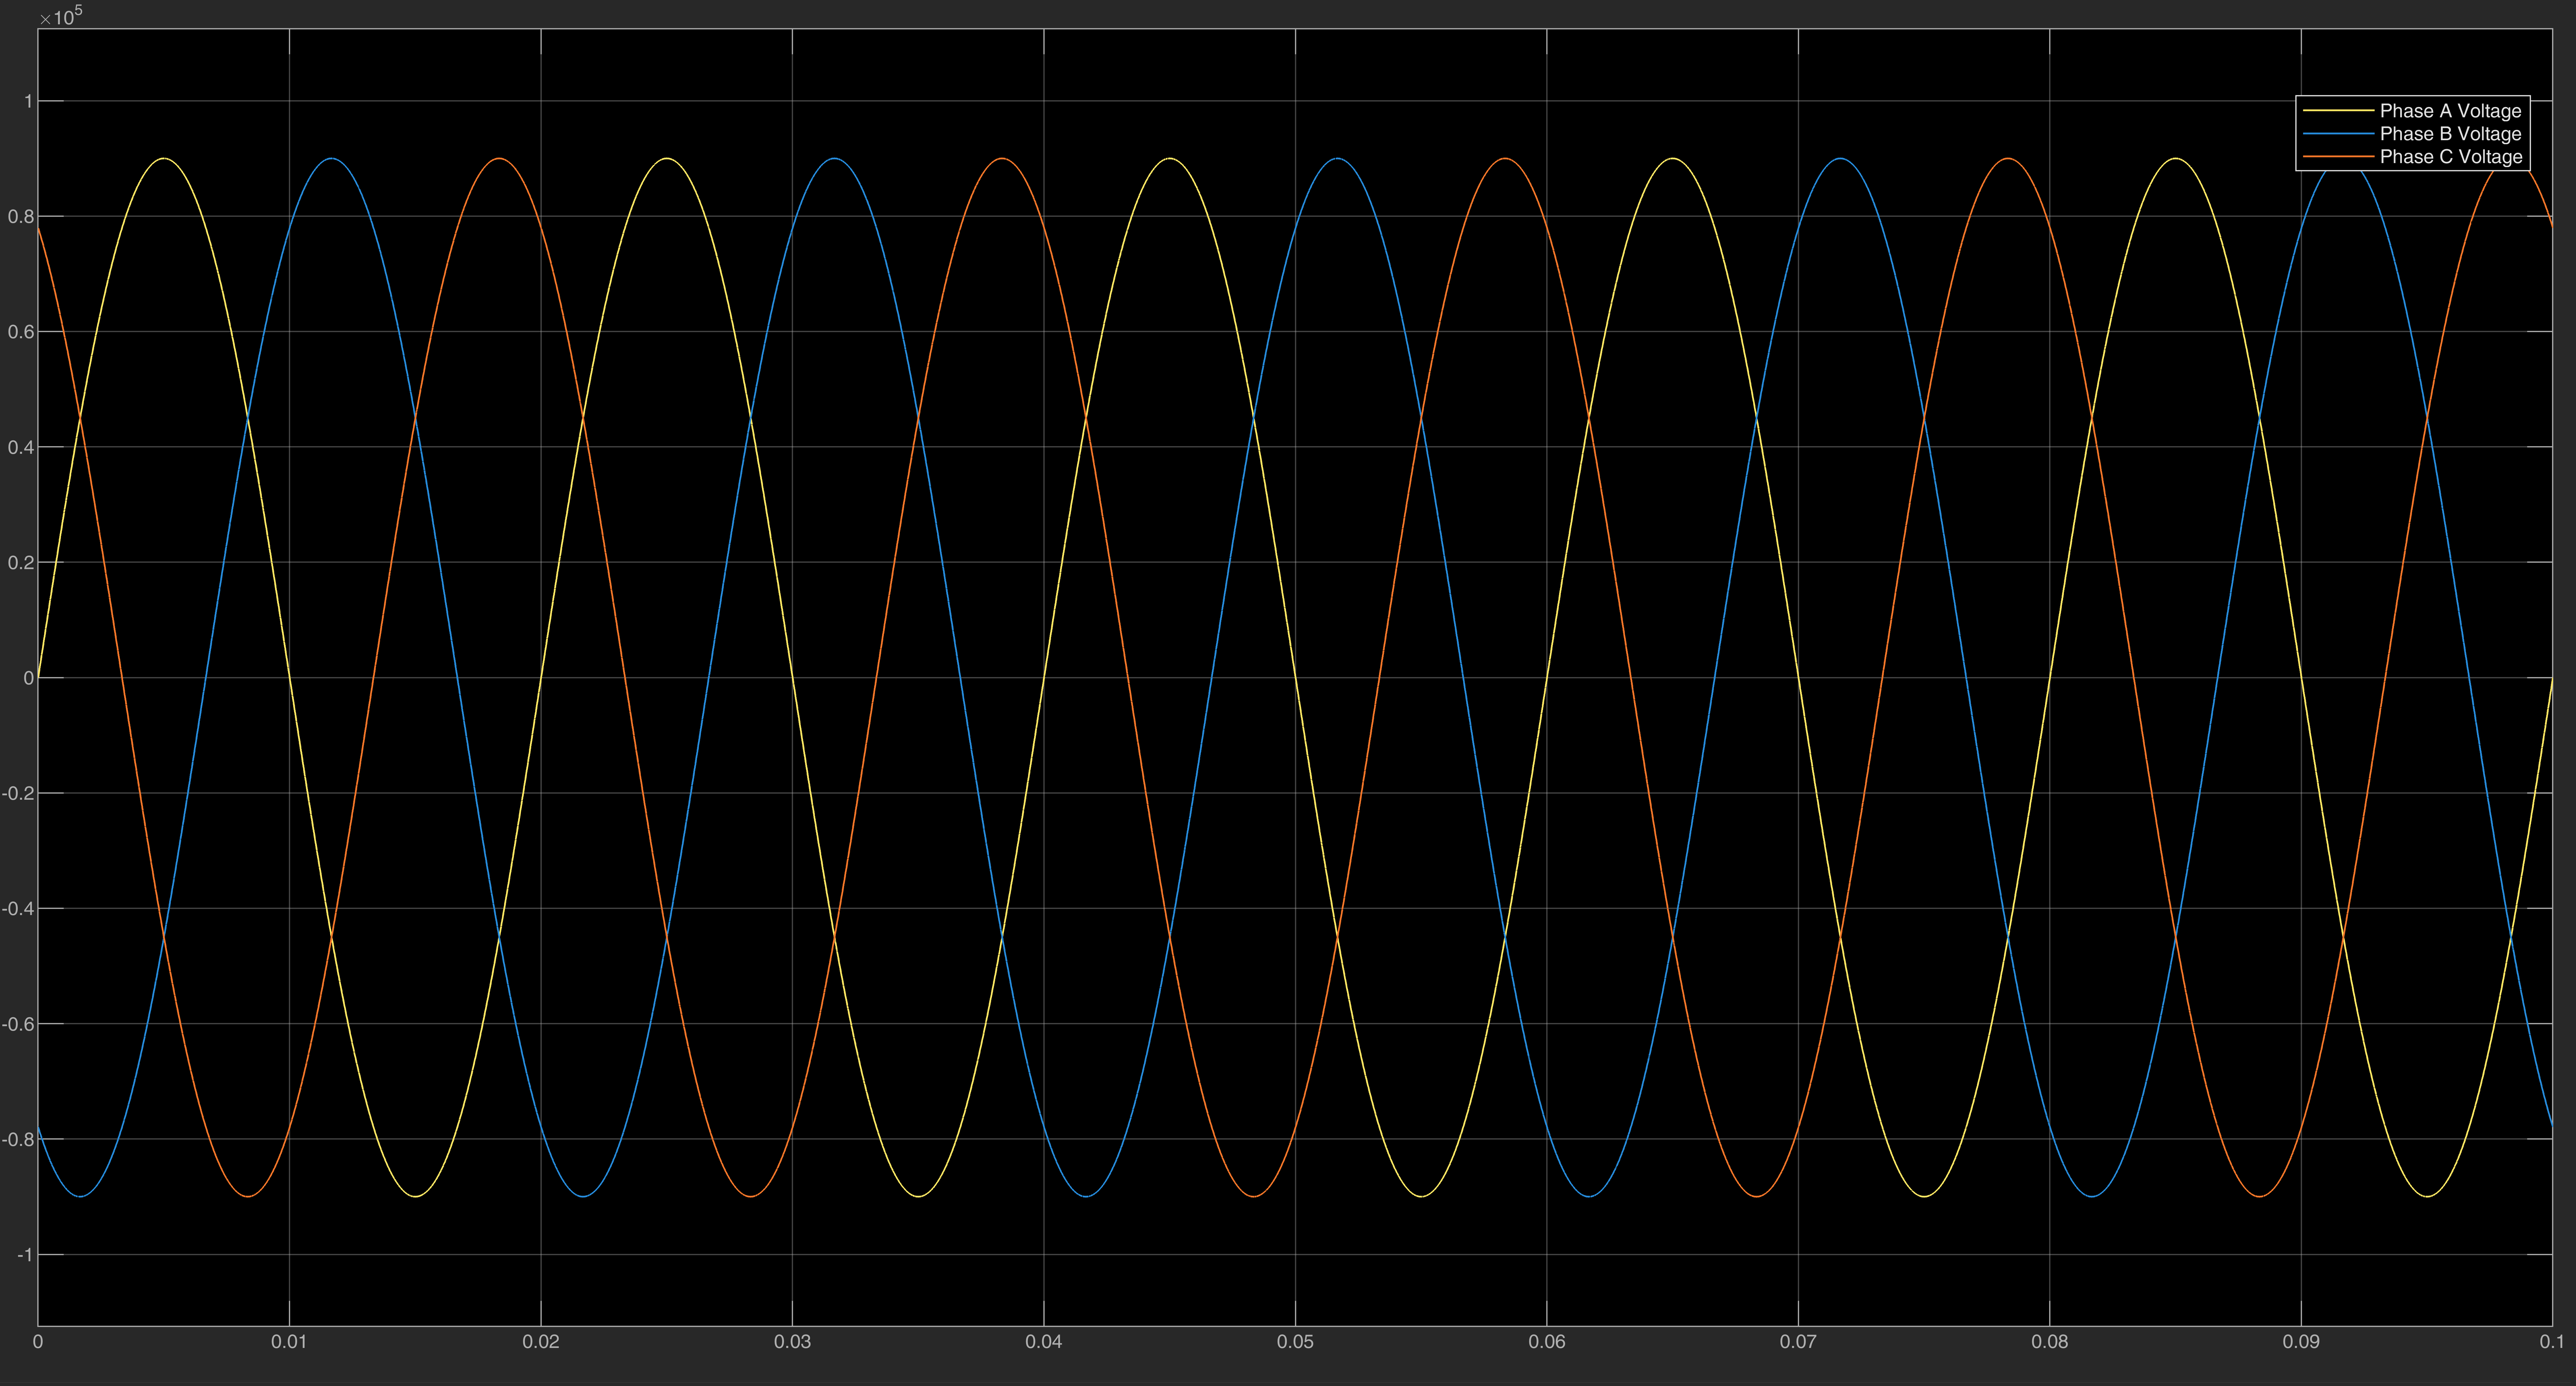
\includegraphics[width=\textwidth]{Grid Voltage_4.png}
        \caption{Grid Voltages}
    \end{subfigure}
    \hfill
    \begin{subfigure}{0.48\textwidth}
        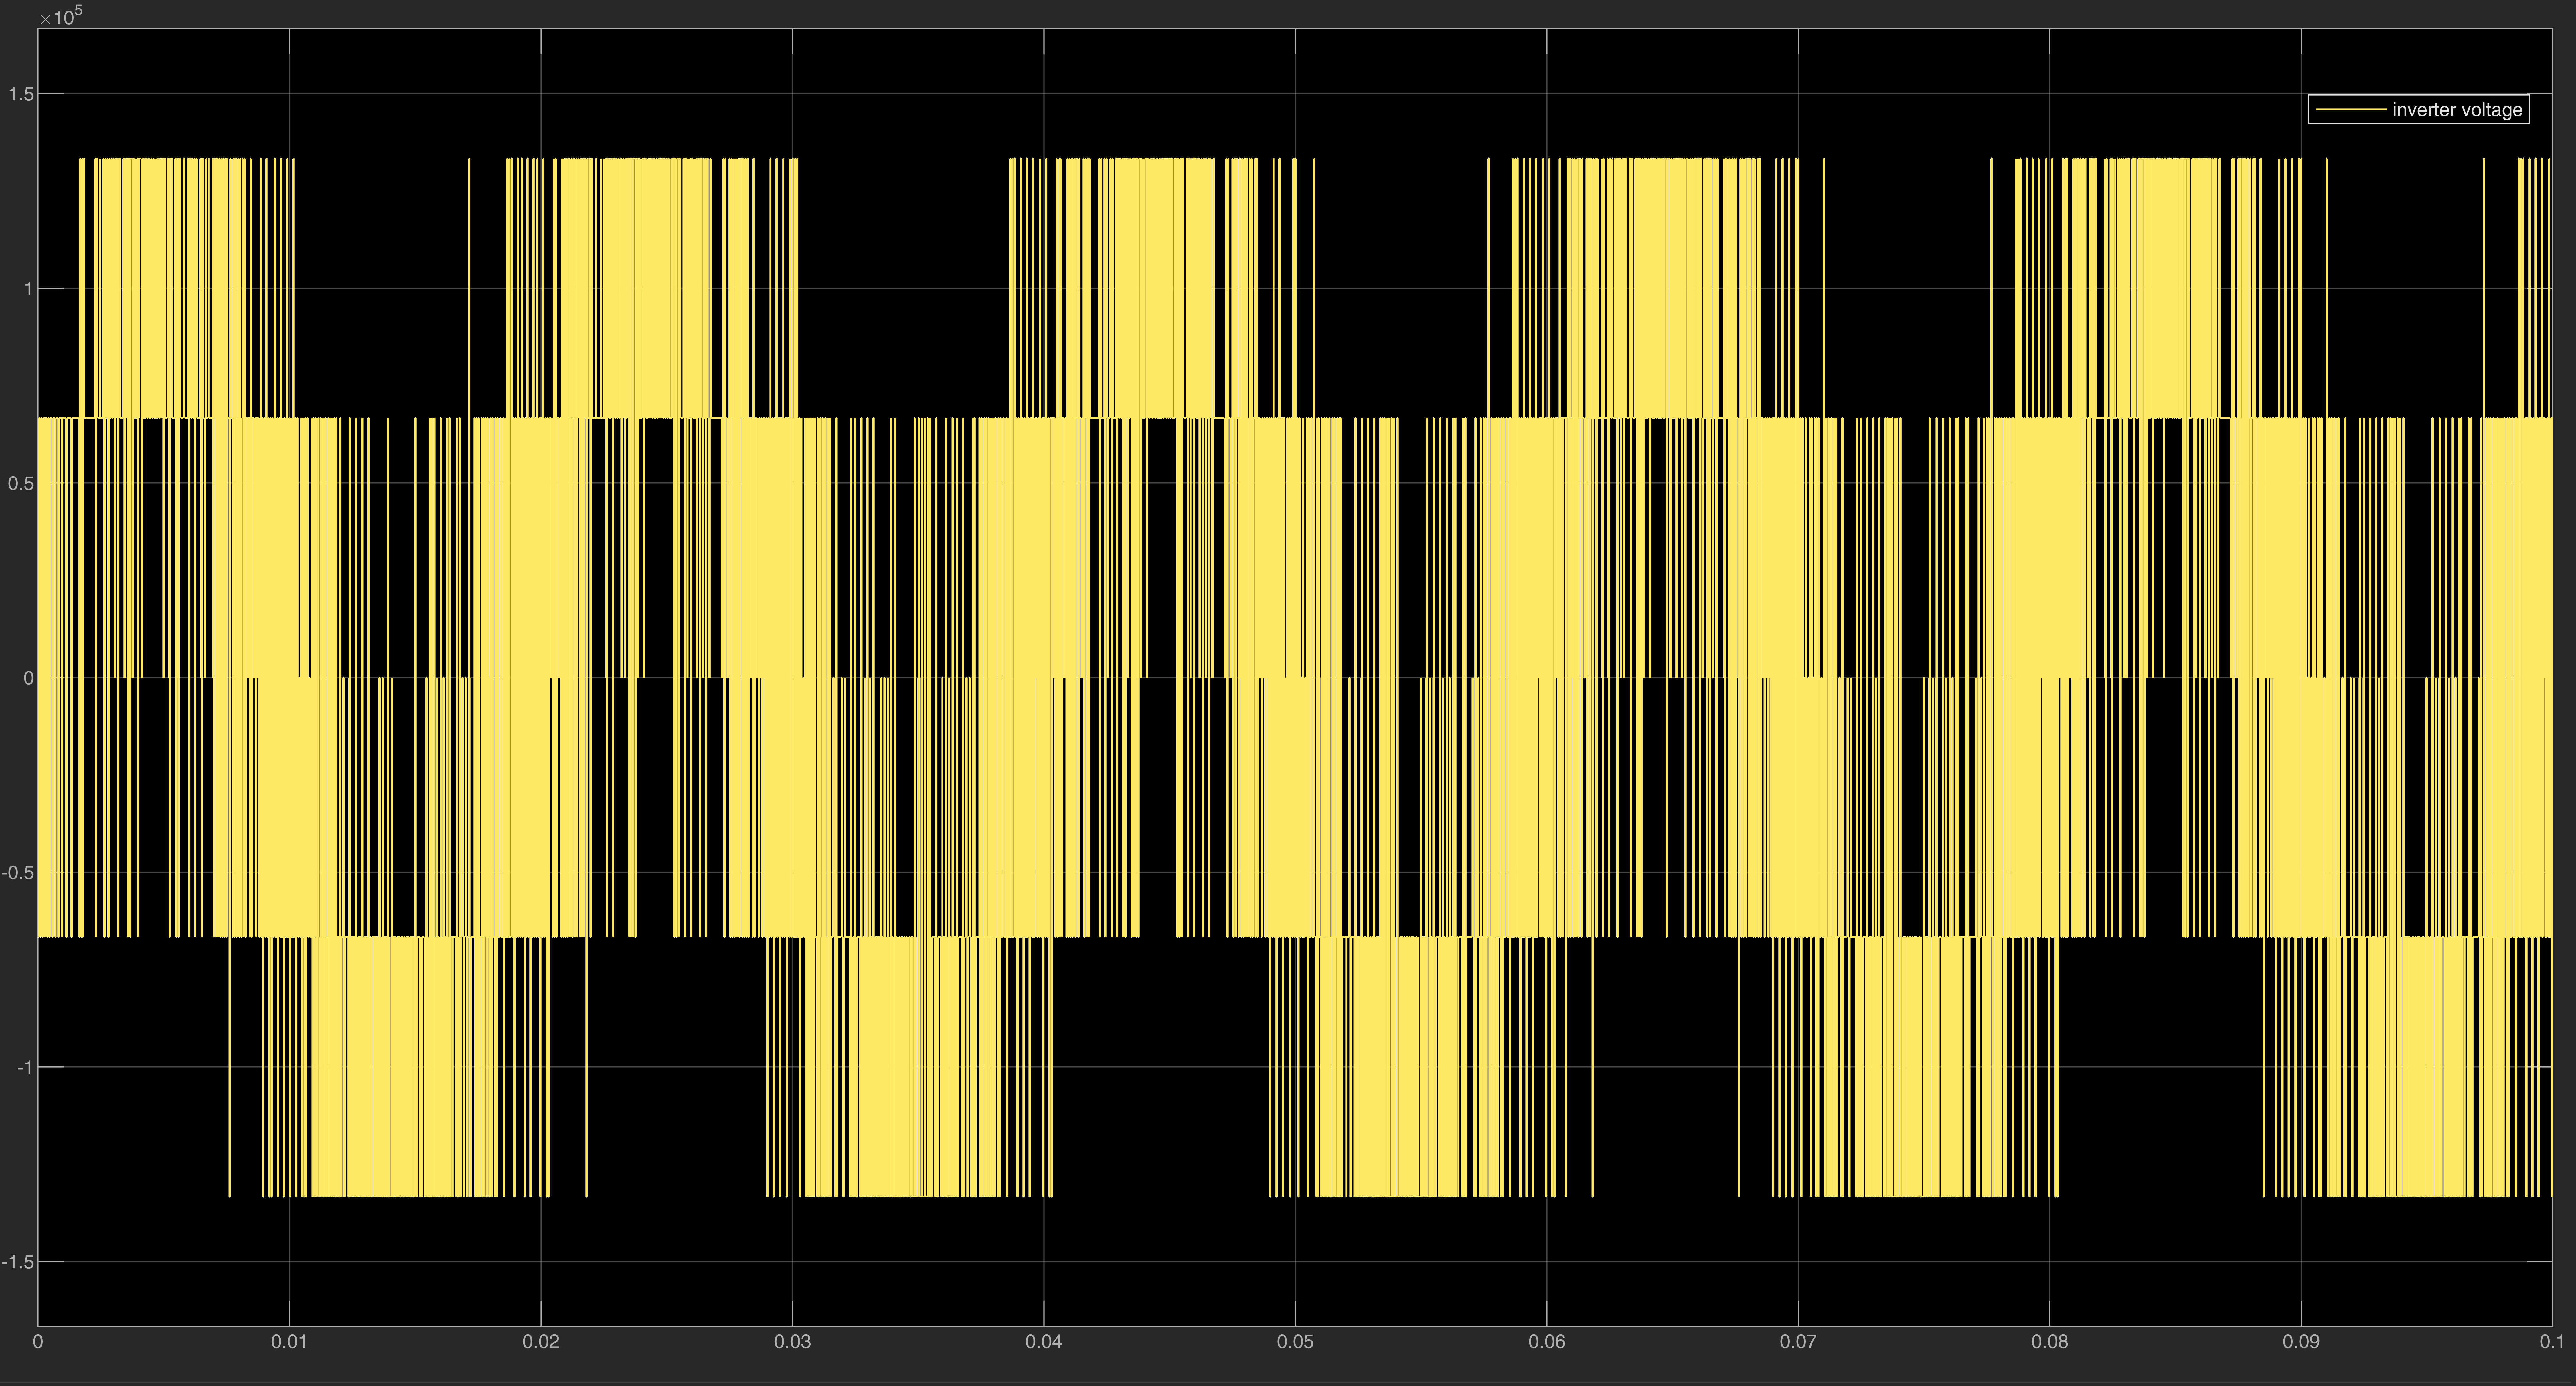
\includegraphics[width=\textwidth]{Inverter Phase Voltage_4.png}
        \caption{Inverter Phase Voltage}
    \end{subfigure}
    \caption{Simulation waveforms for Case 4 (Rectification Mode).}
\end{figure}

% --- Case 5 ---
\subsection{Case 5: Dynamic Step Change (+405 MW to -405 MW)}
The final case investigates the controller's dynamic transient response and stability limits. A severe step change is applied to the active power reference at $t=0.05$ seconds, commanding an instantaneous transition from full inverter mode ($+405\text{ MW}$) to full rectifier mode ($-405\text{ MW}$). 

The hysteresis controller tracks the reversal quickly: the active power flow reverses within a fraction of an AC cycle. This is visually corroborated by the grid current waveform, which abruptly shifts its phase by $180^\circ$ at $t=0.05\text{ s}$. Furthermore, this severe active power transient occurs without inducing significant overshoots or prolonged oscillatory transients in the reactive power profile, which is consistent with decoupled regulation of active and reactive power inherent to this VSC control scheme.

\begin{figure}[H]
    \centering
    \begin{subfigure}{0.48\textwidth}
        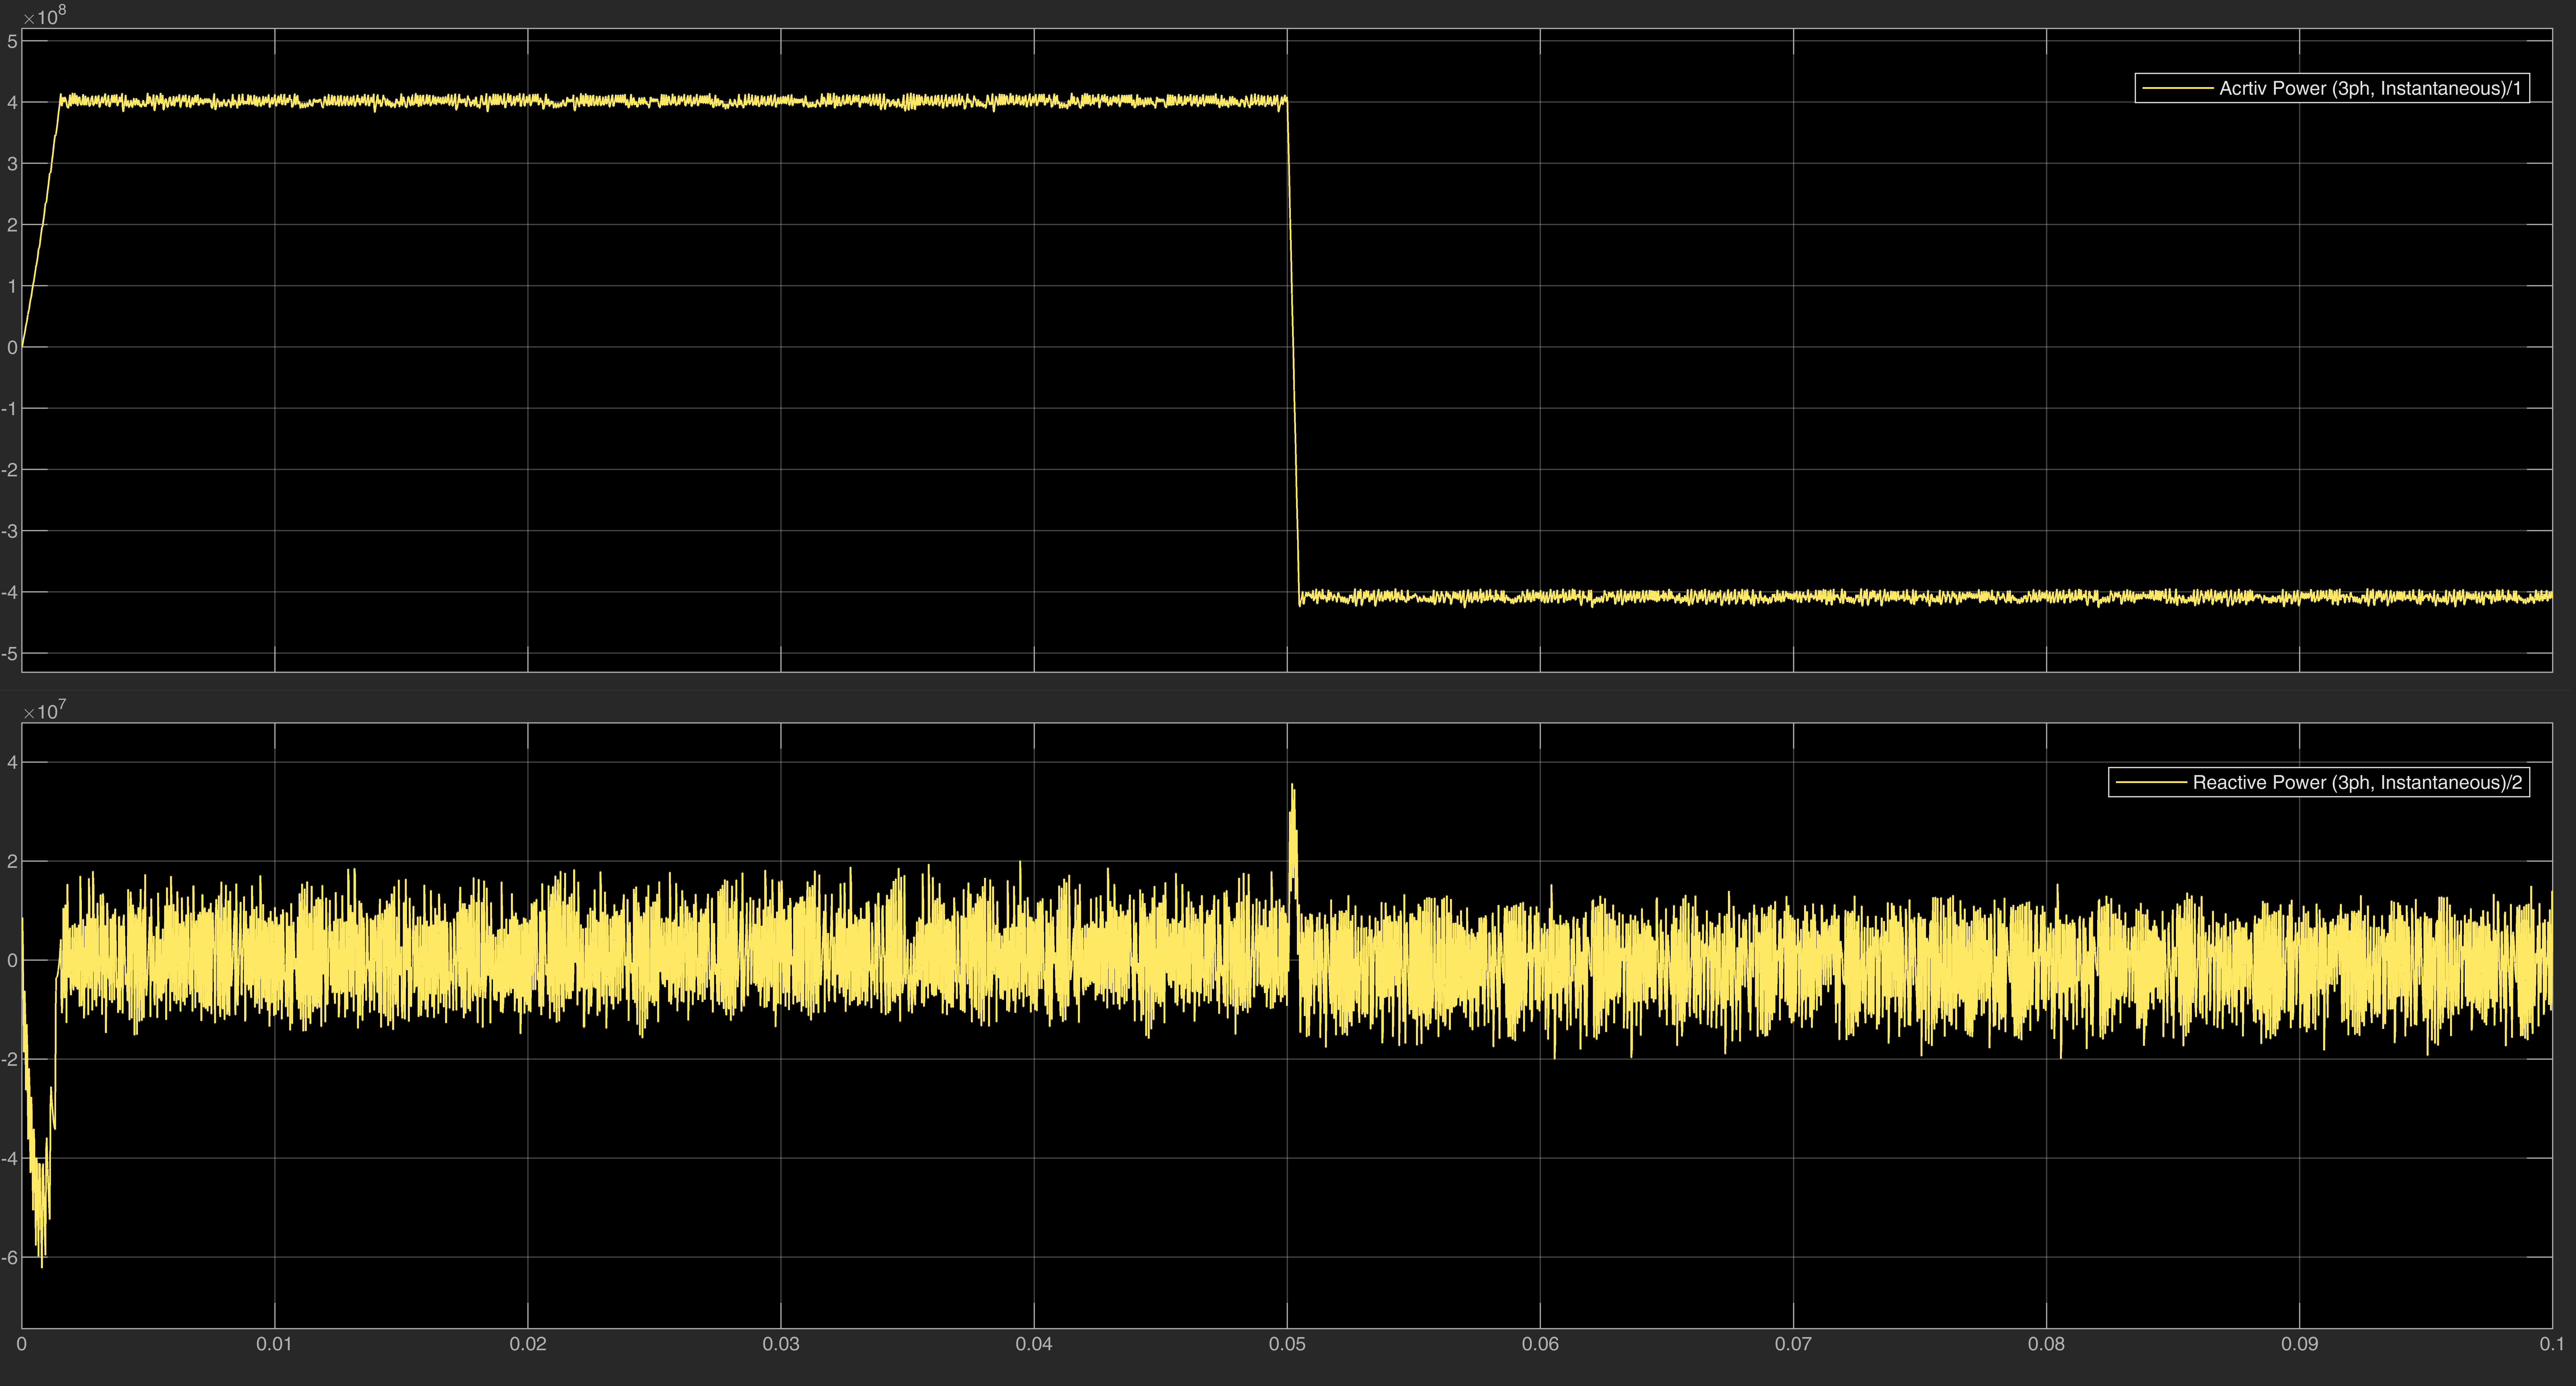
\includegraphics[width=\textwidth]{Grid active and reactive powers_5.png}
        \caption{Active and Reactive Power (Dynamic Response)}
    \end{subfigure}
    \hfill
    \begin{subfigure}{0.48\textwidth}
        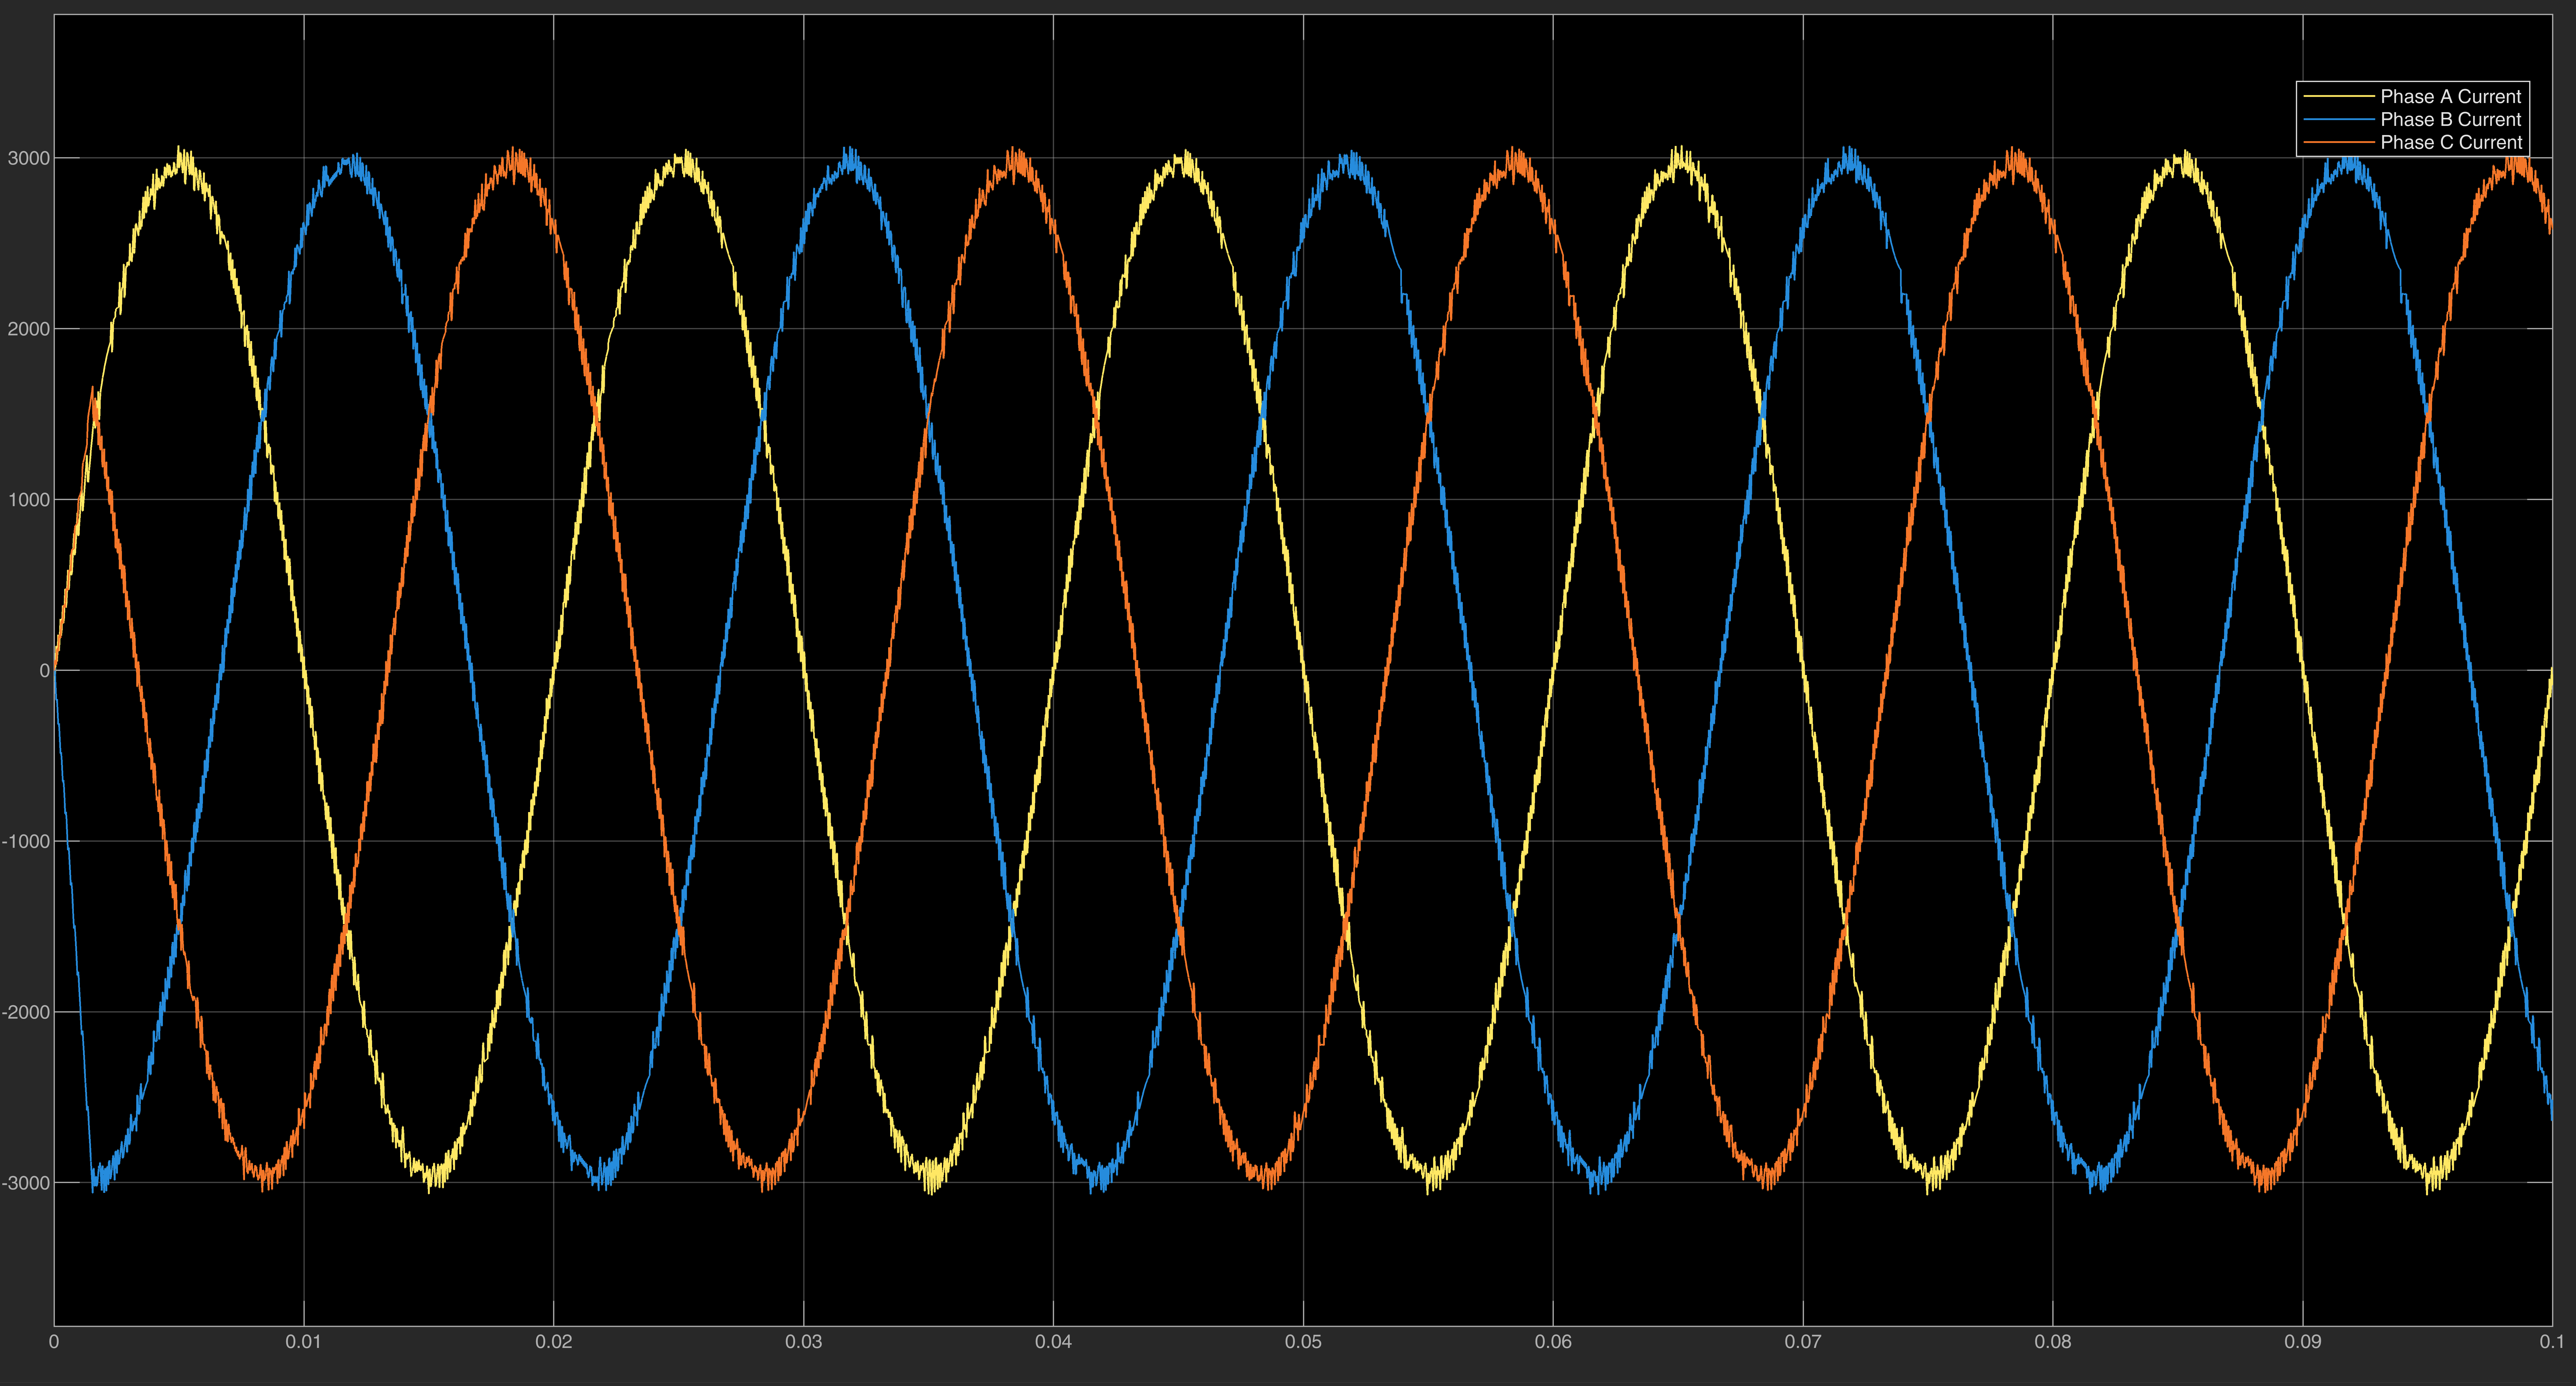
\includegraphics[width=\textwidth]{Grid Currents_5.png}
        \caption{Current Reversal at $t=0.05$ s}
    \end{subfigure}
    \vskip\baselineskip
    \begin{subfigure}{0.48\textwidth}
        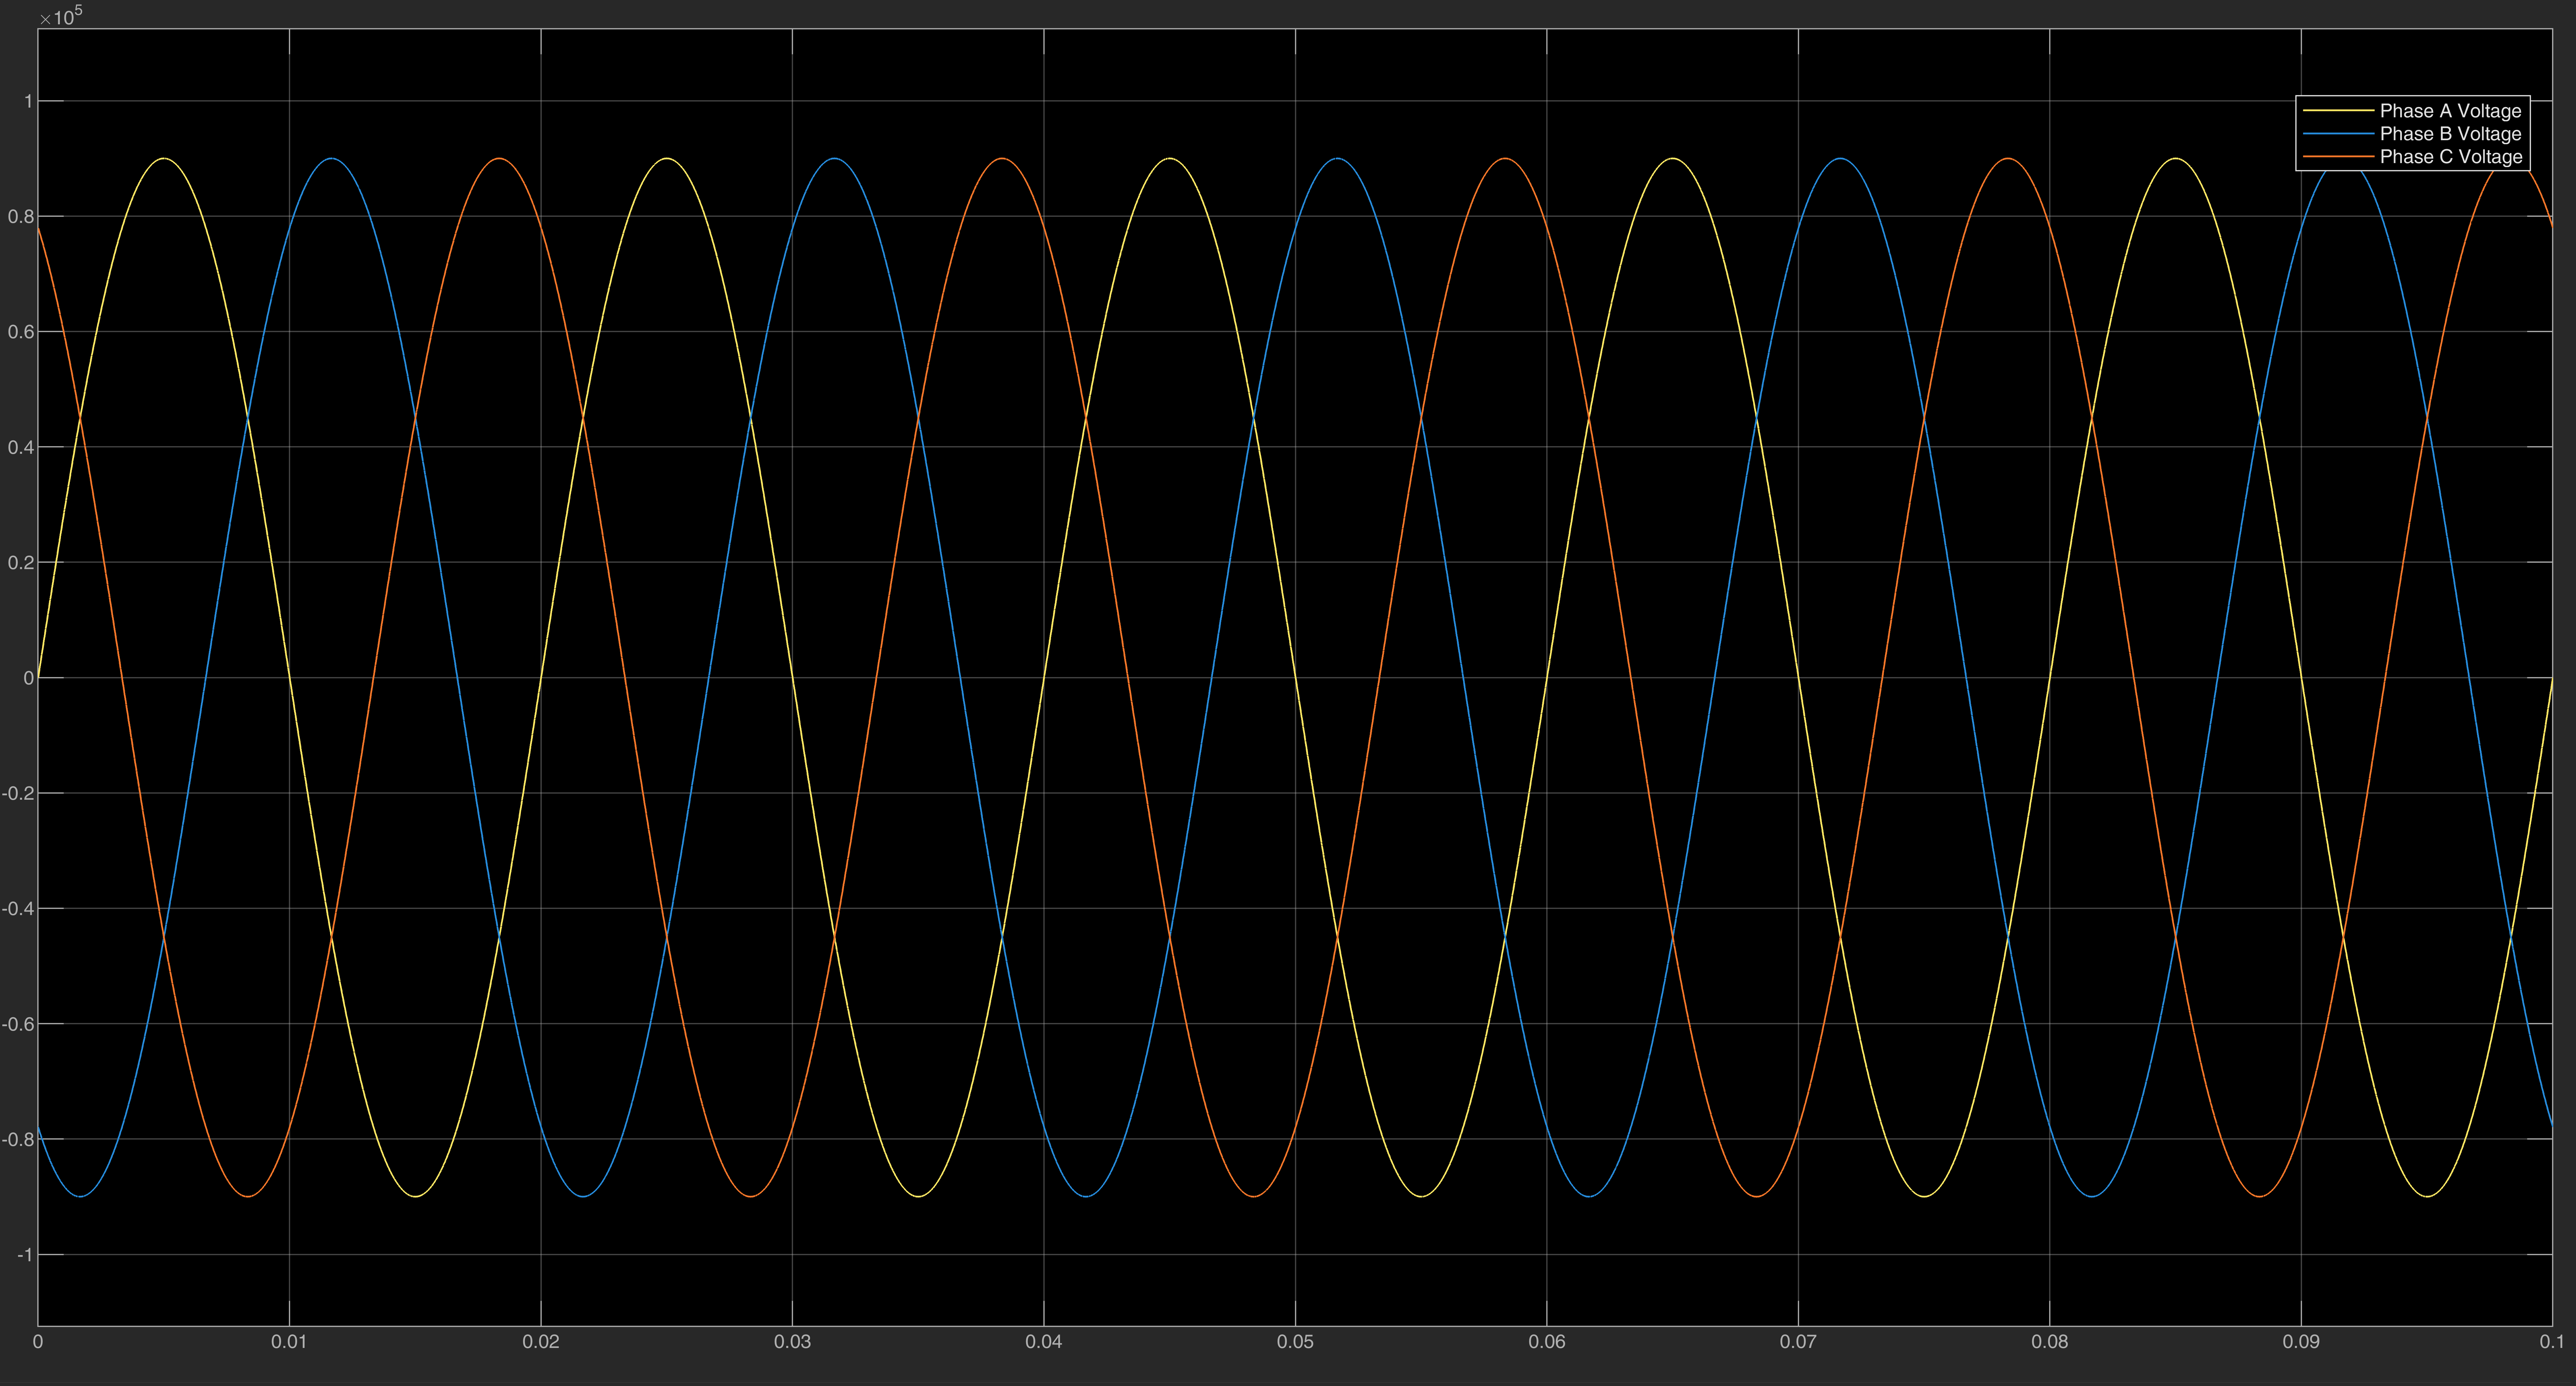
\includegraphics[width=\textwidth]{Grid Voltage_5.png}
        \caption{Grid Voltages}
    \end{subfigure}
    \hfill
    \begin{subfigure}{0.48\textwidth}
        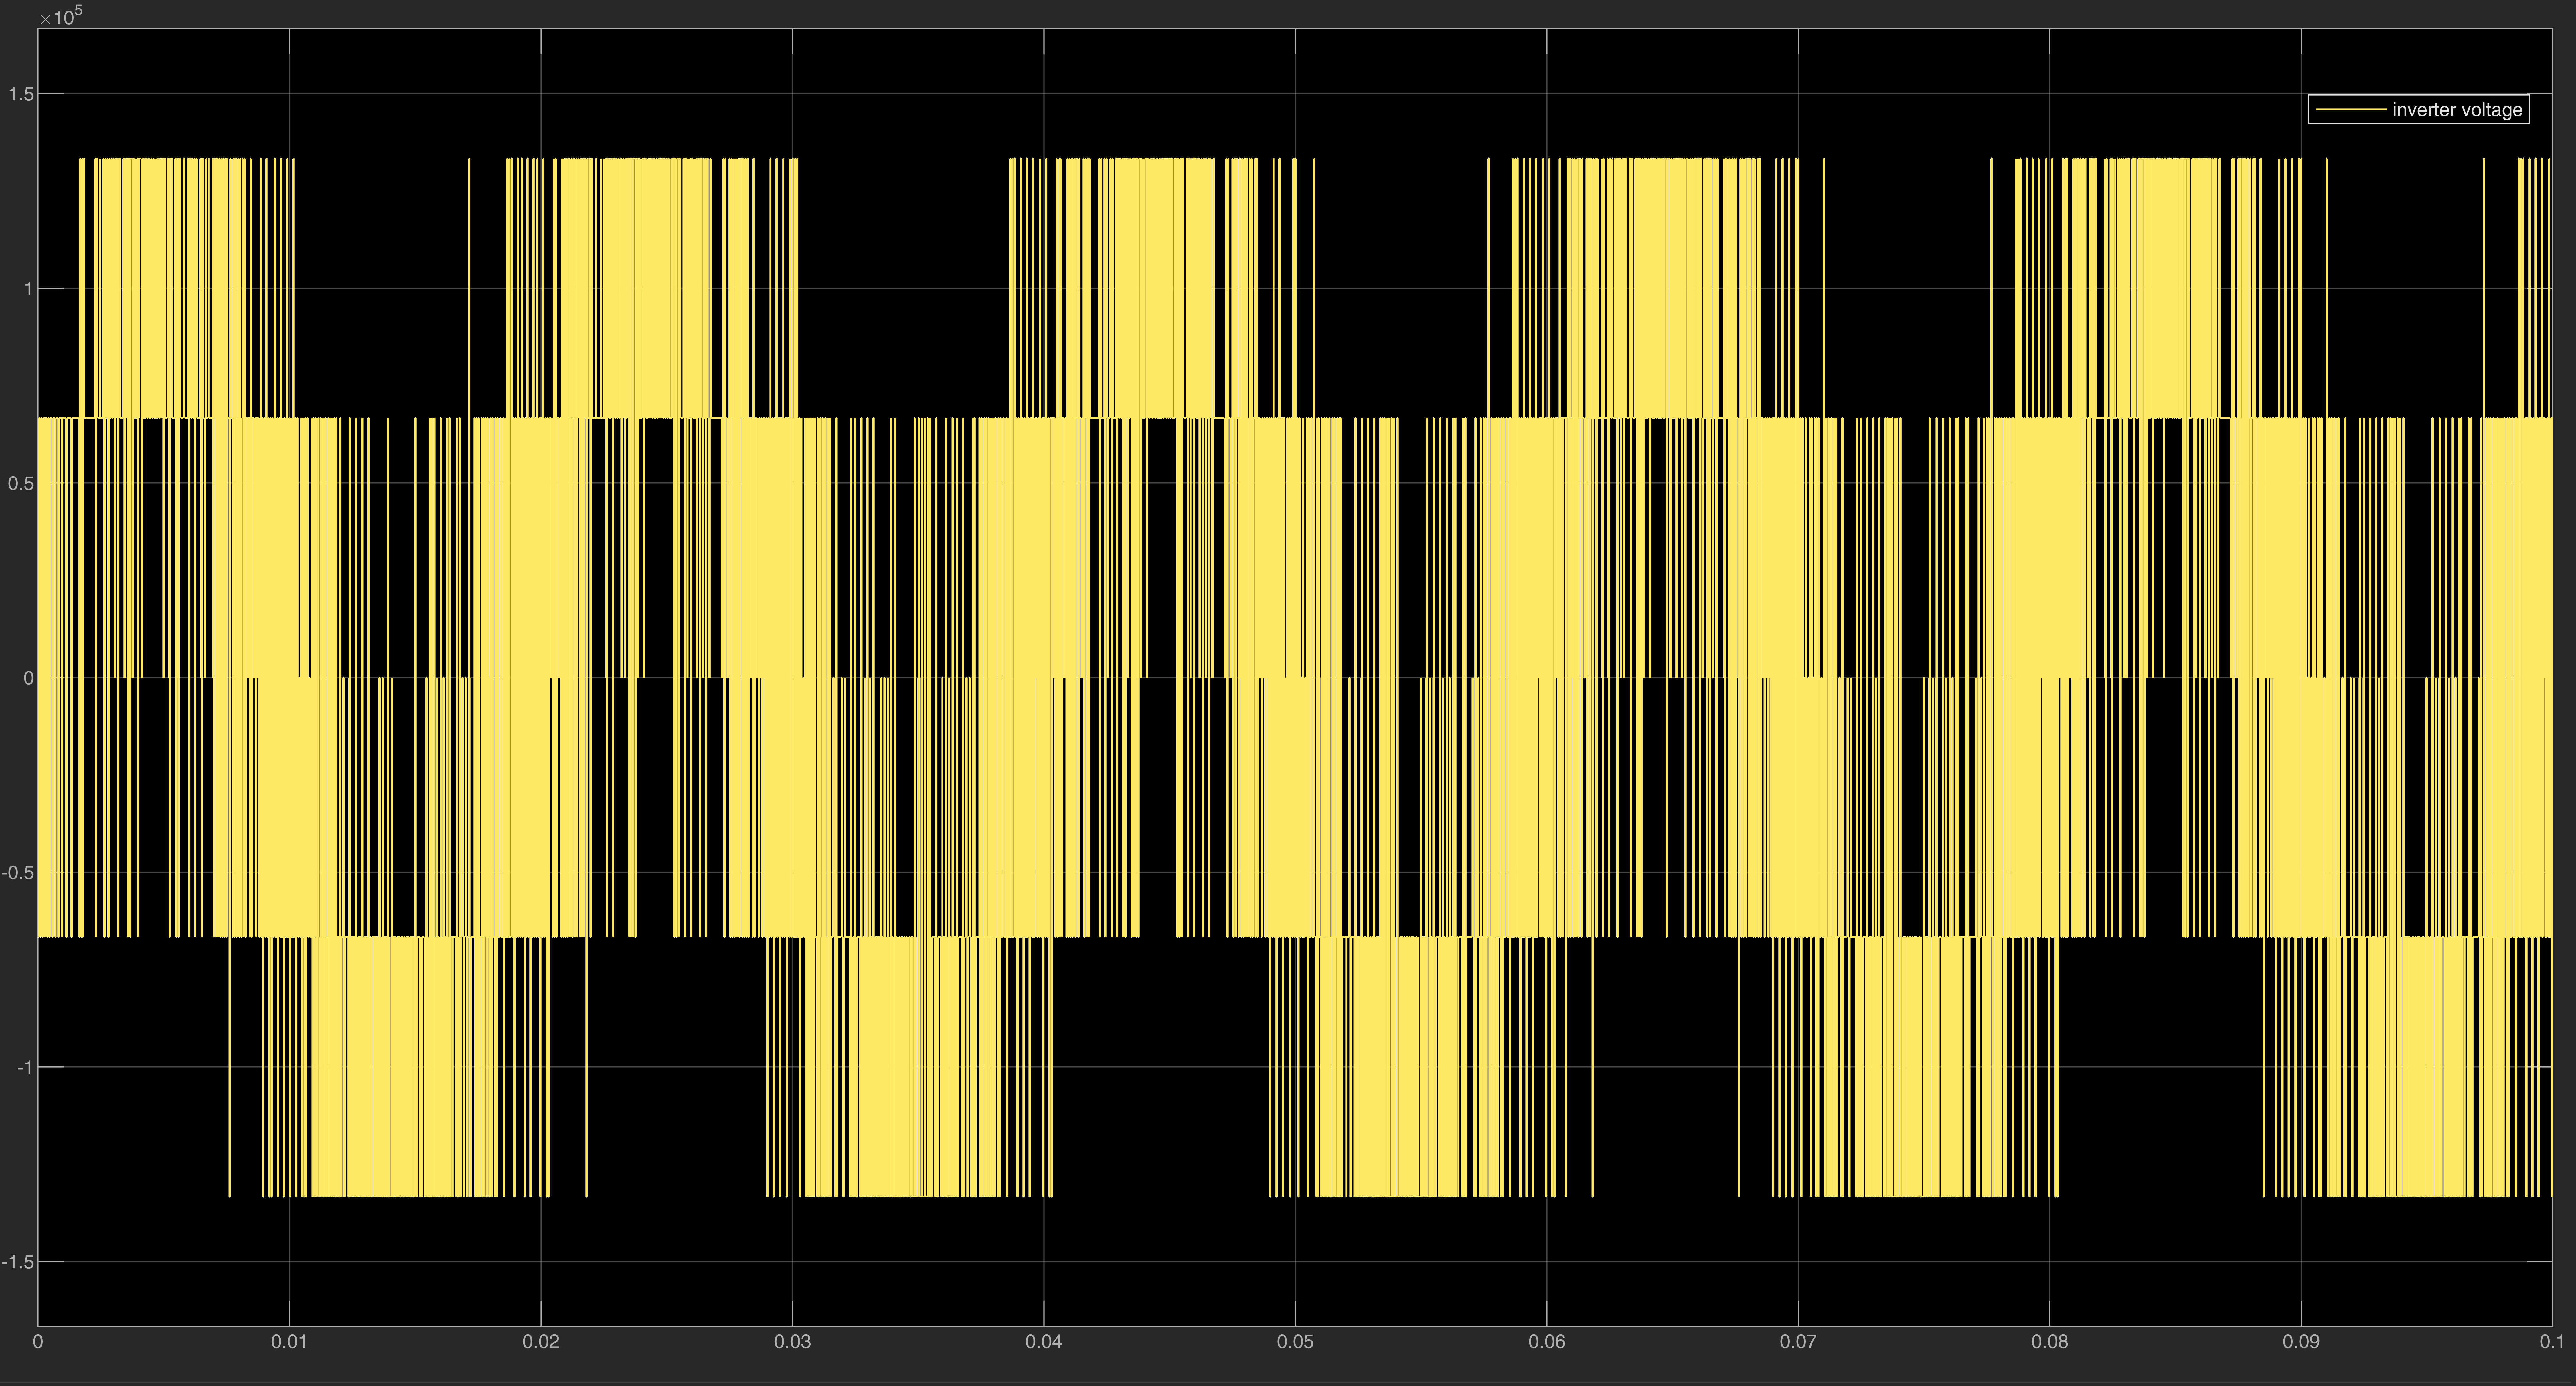
\includegraphics[width=\textwidth]{Inverter Phase Voltage_5.png}
        \caption{Inverter Phase Voltage}
    \end{subfigure}
    \caption{Simulation waveforms for Case 5 (Severe Step Change).}
\end{figure}

\section{Conclusion}
The comprehensive simulation results confirm the effectiveness and accuracy of the Two-Level VSC utilizing Hysteresis Current Control. The mathematical generation of reference currents gave accurate current references. The system successfully tracked all steady-state active and reactive power references independently (Cases 1-4) while maintaining the current tightly within the specified hysteresis band. Furthermore, the controller completed the power reversal within a fraction of an AC cycle (Case 5), which supports its use as a basis for VSC-HVDC studies.

\end{document}